\chapter{\positron\electron pair background}
\label{PairBkg}

\begin{chapterabstract}
 At the International Linear Collider, the collisions of electron and positron beams are accompanied by the production of background particles.
 Unlike at hadron colliders, the main background contribution does not arise from QCD processes and underlying events, but rather from the interaction of the colliding beam's electromagnetic fields.
 The created secondary \positron\electron pairs form a significant background, the so-called pair background, for the inner detectors, and therefore need to be studied in great detail.
 This chapter discusses the effect of the ILC beam parameters on the pair background, and the impact of the \positron\electron pairs on the \sid detector.
\end{chapterabstract}

As discussed in Section~\ref{BeamBeam}, the pair background is a high cross section process from beam-beam interactions and the main source of background at the ILC.
The secondary electrons and positrons show a characteristic density distribution, which reaches to the inner layers of the \sid vertex detector barrel.
The impact on the \sid detector is studied with respect to the timing, the hit distribution, and the arising detector occupancy.
These impacts are, however, dependent on several factors, such as the ILC beam parameters.
For the proposed change in the beam parameters for the ILC stage at \SI{250}{\GeV}, the effect on the pair background has been analyzed in detail.
The results of these studies, which are explained throughout the following sections, are essential for the design choices of the accelerator and the \sid detector.

\section{The background generator GuineaPig}
\label{PairBkg:GuineaPig}
For studying the effects of the pair background, \positron\electron pairs from beam-beam interactions were generated with the Monte Carlo (MC) background event generator \guineapig~\cite{Schulte:1997nga} version 1.4.4. 
When providing the accelerator beam parameters, the pair background events of one bunch crossing are simulated and stored in an ASCII output file.
The parameters used for generating the pair background for this thesis are given in Appendix~\ref{Appendix:Pairs:GuineaPig}. 
\\Since the ASCII files cannot directly serve as input to a full \geant~\cite{geant_ref,geant_ref2} detector simulation, a conversion tool was developed for the analysis studies presented in this thesis, and instructions on its usage are available in~\cite{Confluence}. 
The tool converts the ASCII output to one of the following file formats, common for ILC detector simulations: stdhep~\cite{stdhep} or slcio~\cite{LCIO}.
These file formats are directly applicable with the \geant based simulation tool \slic~\cite{Graf:2006ei}, which simulates interactions of the input particles with matter.
The geometry of the simulated world is described in a human-readable format.
The flexible geometry description allows the simulation of particle interactions with individual detector geometries.
To this end, the geometry description file ``sidloi3'' of the \sid detector, which was used for the simulation studies in this and in the following chapters, was developed for the \sid Letter of Intent~\cite{LoI} and is based on the detector design described in Section~\ref{ILC:SiD} and in~\cite[p. 69 ff]{TDR4}.
The \sid geometry is visualized in an event display of the pair background for a center-of-mass energy of \SI{500}{\GeV} in Figure~\ref{fig:PairBkg:wired4}.
As will be discussed in the following sections, the simulation of the pair background reveals that the pairs populate mainly the inner and the forward \sid subdetectors, but also the calorimeter endcap layers around the beam pipe.
 \begin{figure}[h]
 \centering
  \begin{subfigure}[b]{0.32\textwidth}
   \centering
    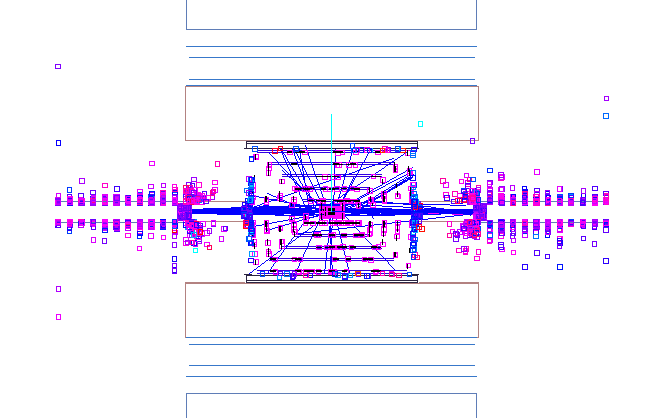
\includegraphics[width=\textwidth]{Figures/Pairs/Event_display_ILC500_rhoz_view_inverted.png}
   \caption{Parallel view}
   \end{subfigure}
   \hfill
    \begin{subfigure}[b]{0.31\textwidth}
   \centering
    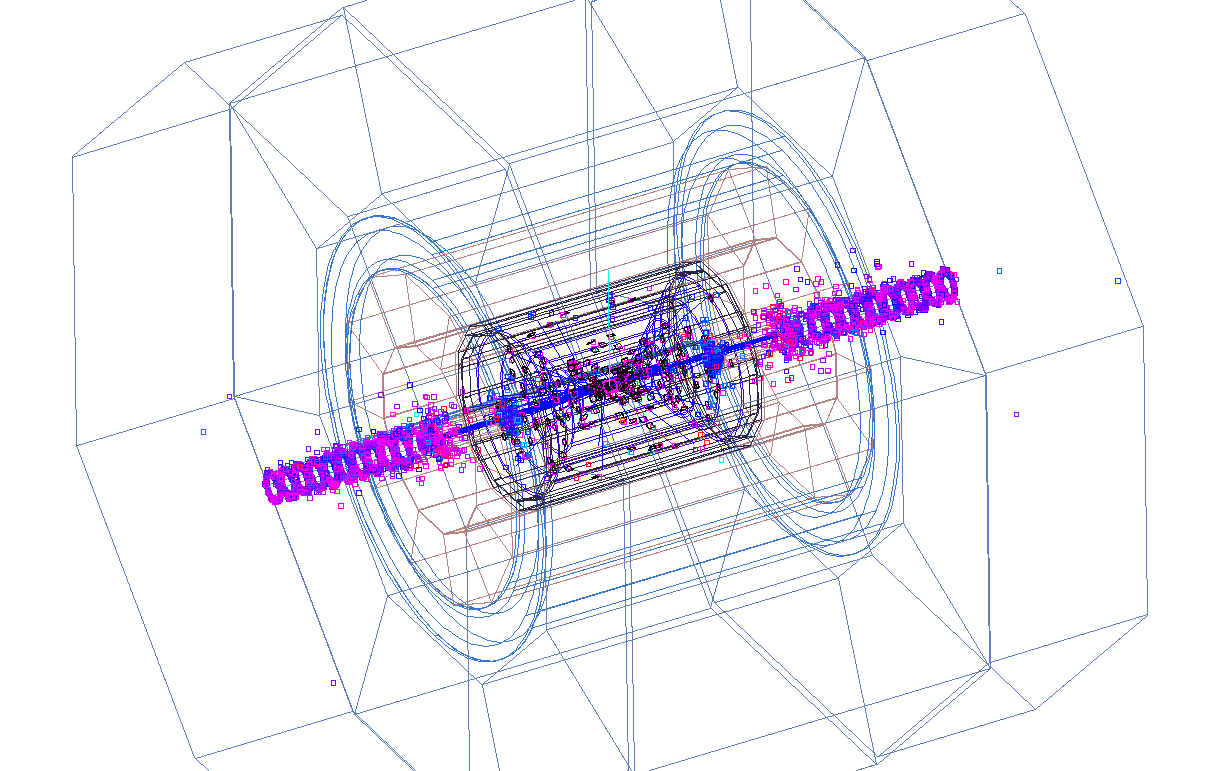
\includegraphics[width=0.96\textwidth]{Figures/Pairs/Event_display_ILC500_3D_view2_inverted.png}
   \caption{3D view}
   \end{subfigure}
    \hfill
    \begin{subfigure}[b]{0.3\textwidth}
   \centering
    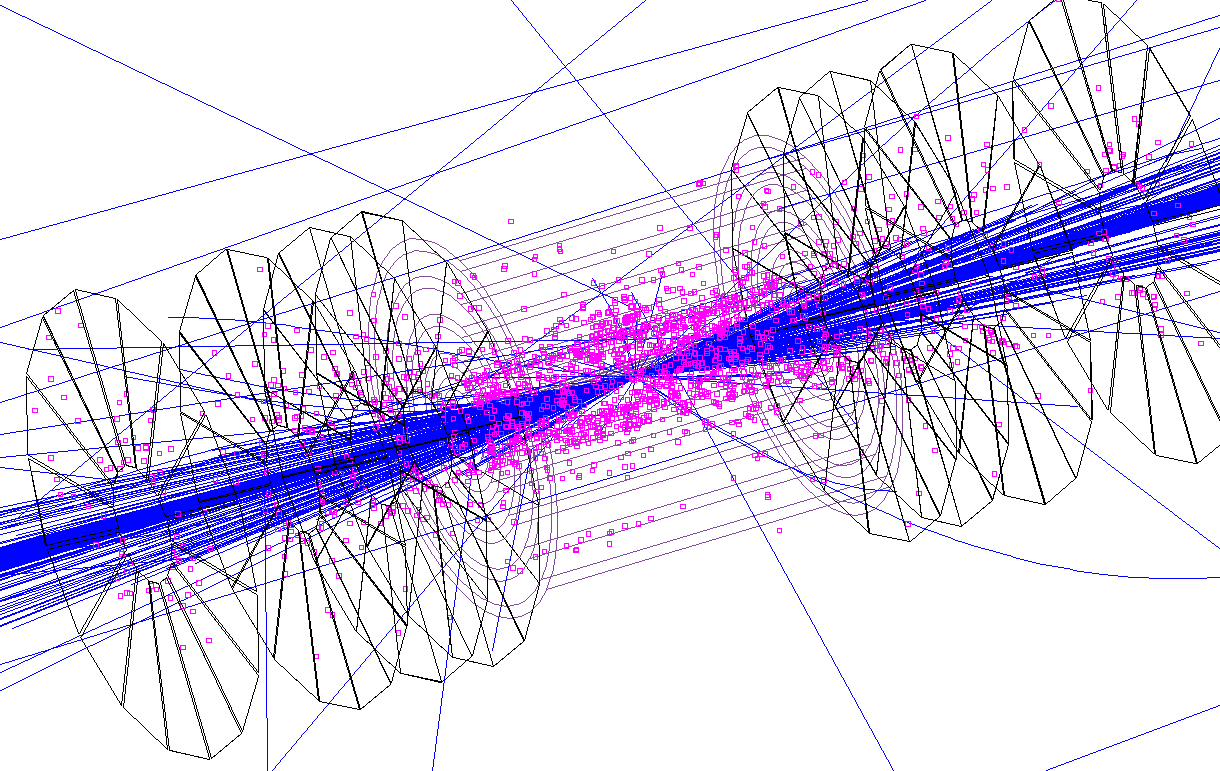
\includegraphics[width=0.96\textwidth]{Figures/Pairs/Event_display_ILC500_vertex_3D_view2_inverted.png}
   \caption{3D view of the vertex detector}
   \end{subfigure}
   \caption[Pair background event displays]{Event displays of the pair background in the 
   \sid detector for the ILC stage at a center-of-mass energy of \SI[detect-all]{500}{\GeV}. 
   The event displays were made with WIRED4~\cite{Wired4}.
   \\Figure (a) shows the whole \sid detector in a parallel view.
   Figures (b) and (c) show a three-dimensional visualization.
   \\Hits from the pair background particles can mainly be found in the inner and the forward detectors, but also around the beam pipe in all layers of the calorimeter endcaps.
   }
   \label{fig:PairBkg:wired4}
 \end{figure}

\section{Pair background characteristics}
\label{PairBkg:helix}
Analyzing the generated pair background events, it becomes apparent that the \positron\electron pairs have a low transverse momentum.
Figure~\ref{fig:PairBkg:Momentum} shows the distribution of their longitudinal and transverse momentum for the two ILC stages at \SI{250}{\GeV} and \SI{500}{\GeV} center-of-mass energy.
The longitudinal momentum of the \positron\electron pairs reaches roughly \SI{80}{\percent} of the beam energy, whilst the transverse momentum extends to only \SI{0.8}{\GeV} for the ILC250, and \SI{1.6}{\GeV} for the ILC500.
 \begin{figure}
 \centering
  \begin{subfigure}[b]{0.49\textwidth}
   \centering
    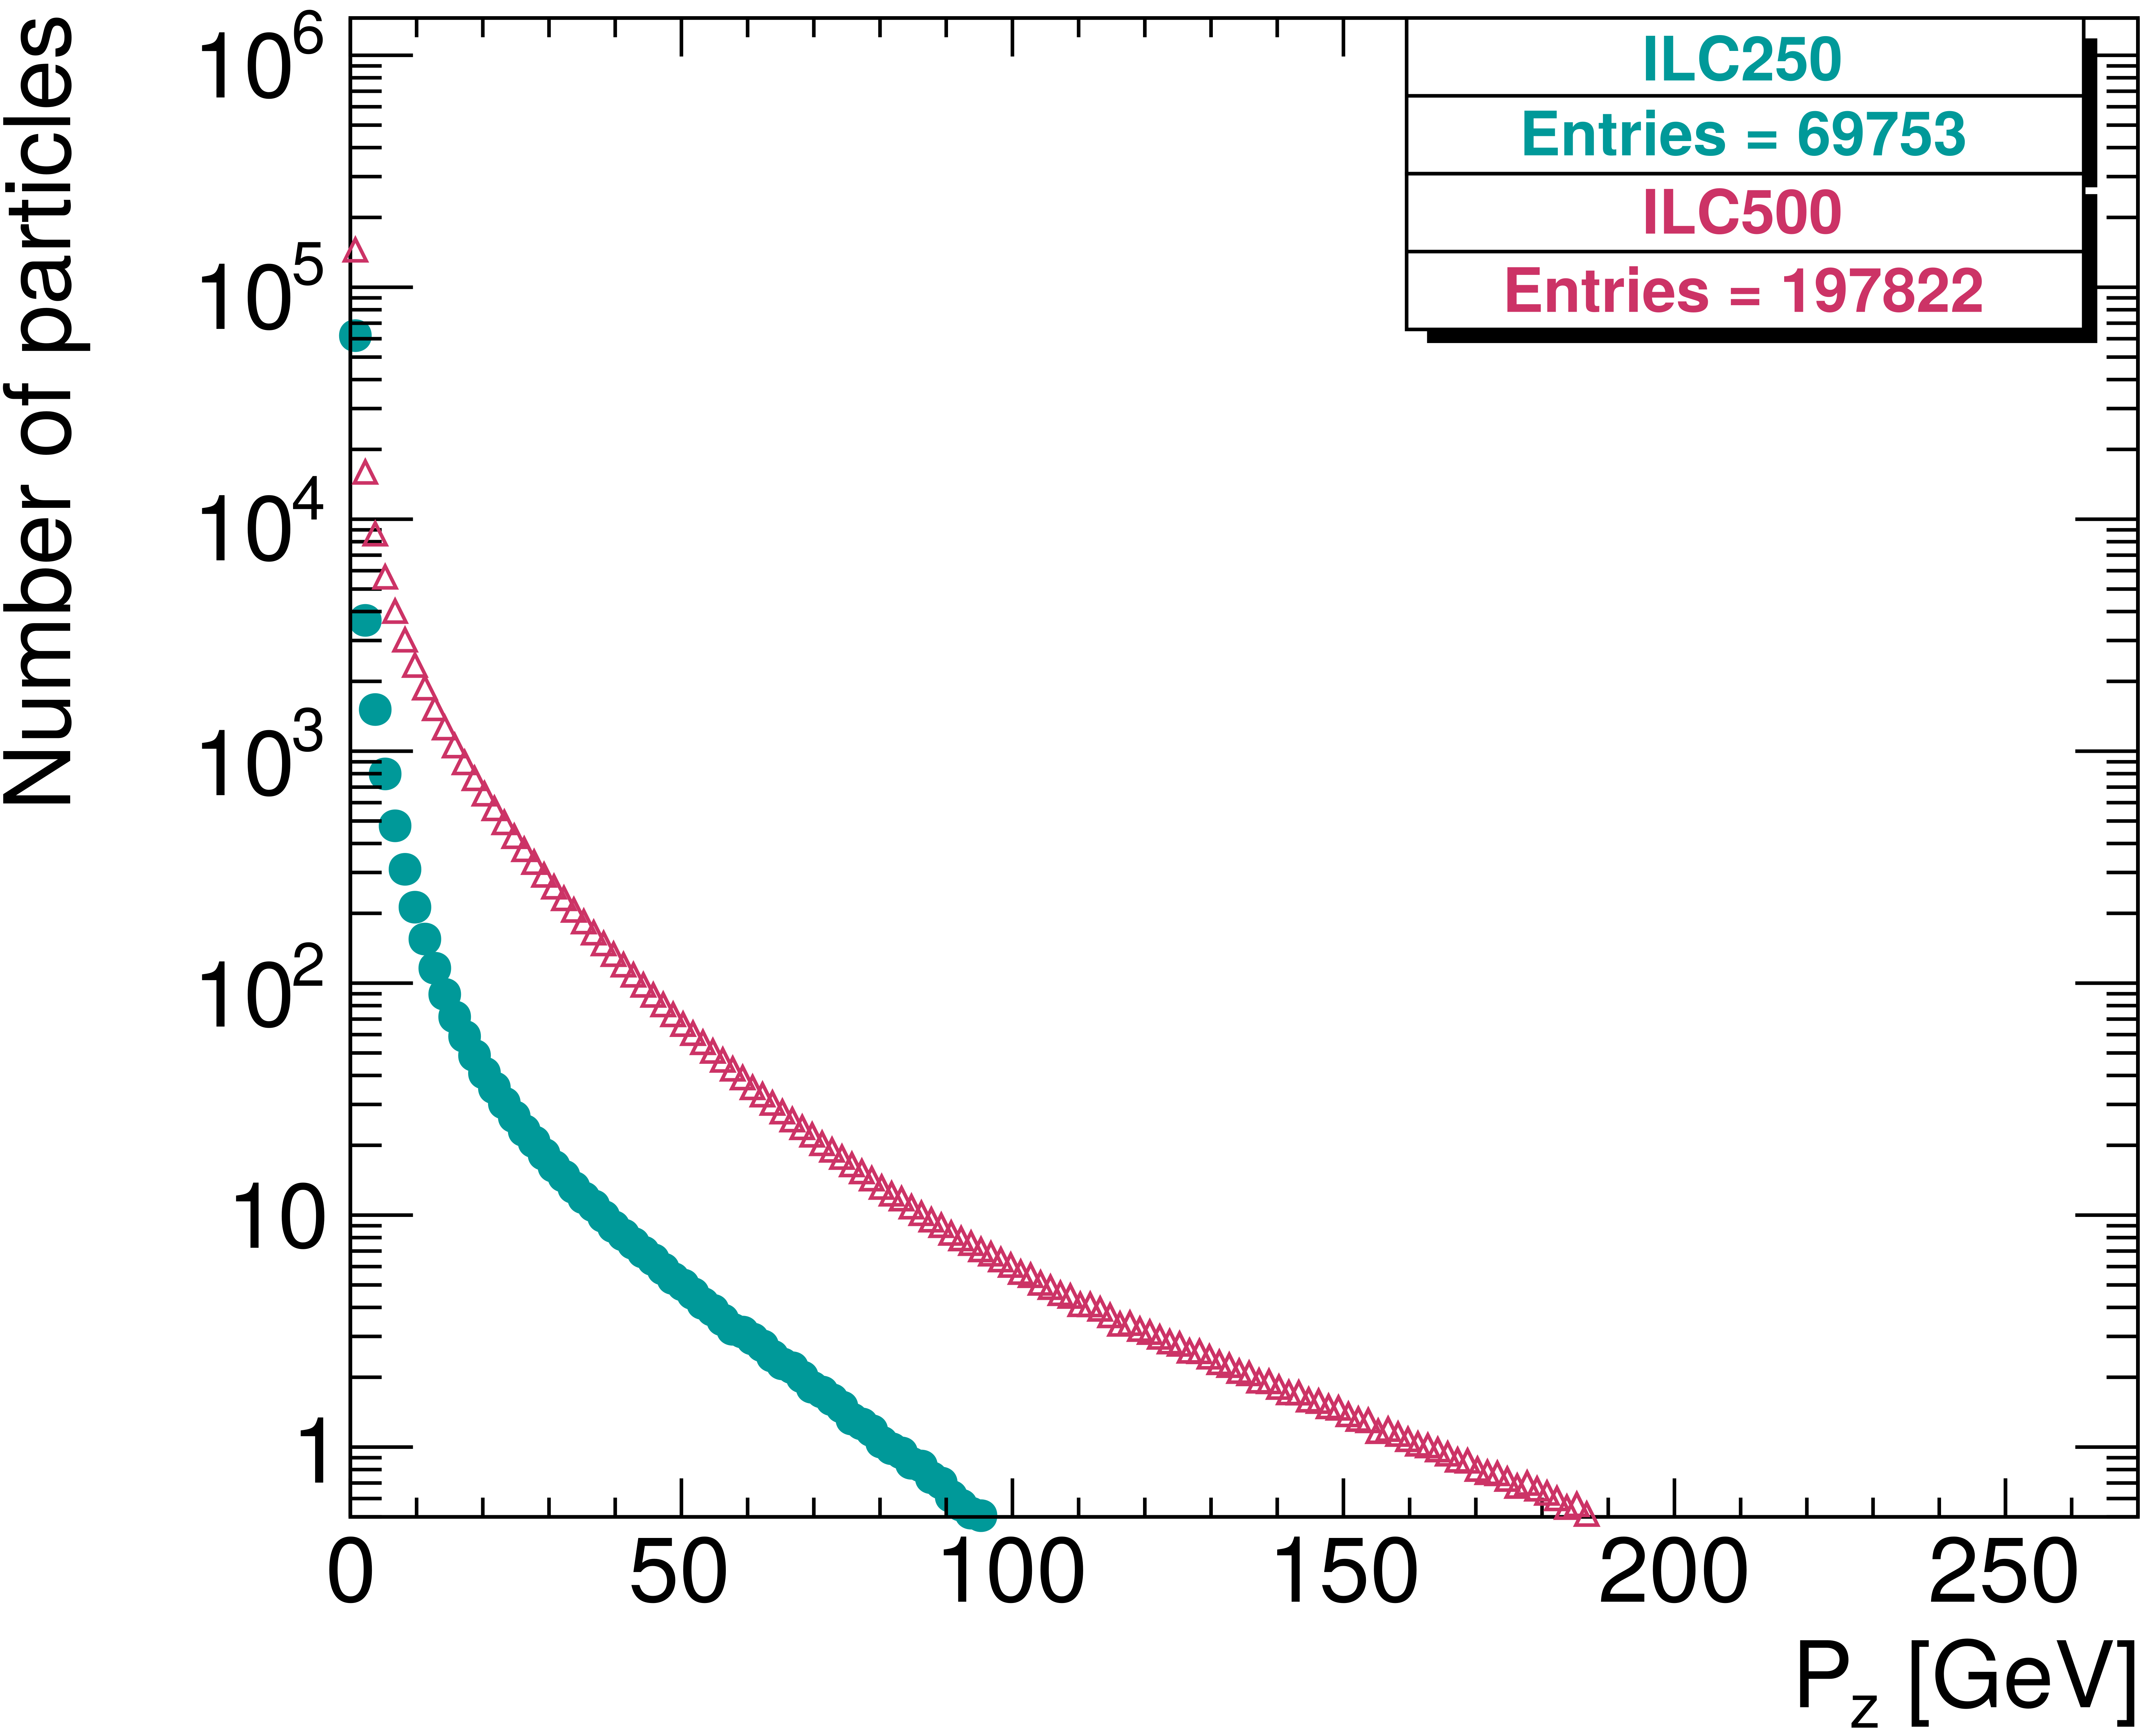
\includegraphics[width=0.95\textwidth]{Figures/Pairs/250_500_pairs_comparison_Pz.png}
   \caption{Longitudinal momentum}
   \end{subfigure}
   \hfill
    \begin{subfigure}[b]{0.49\textwidth}
   \centering
    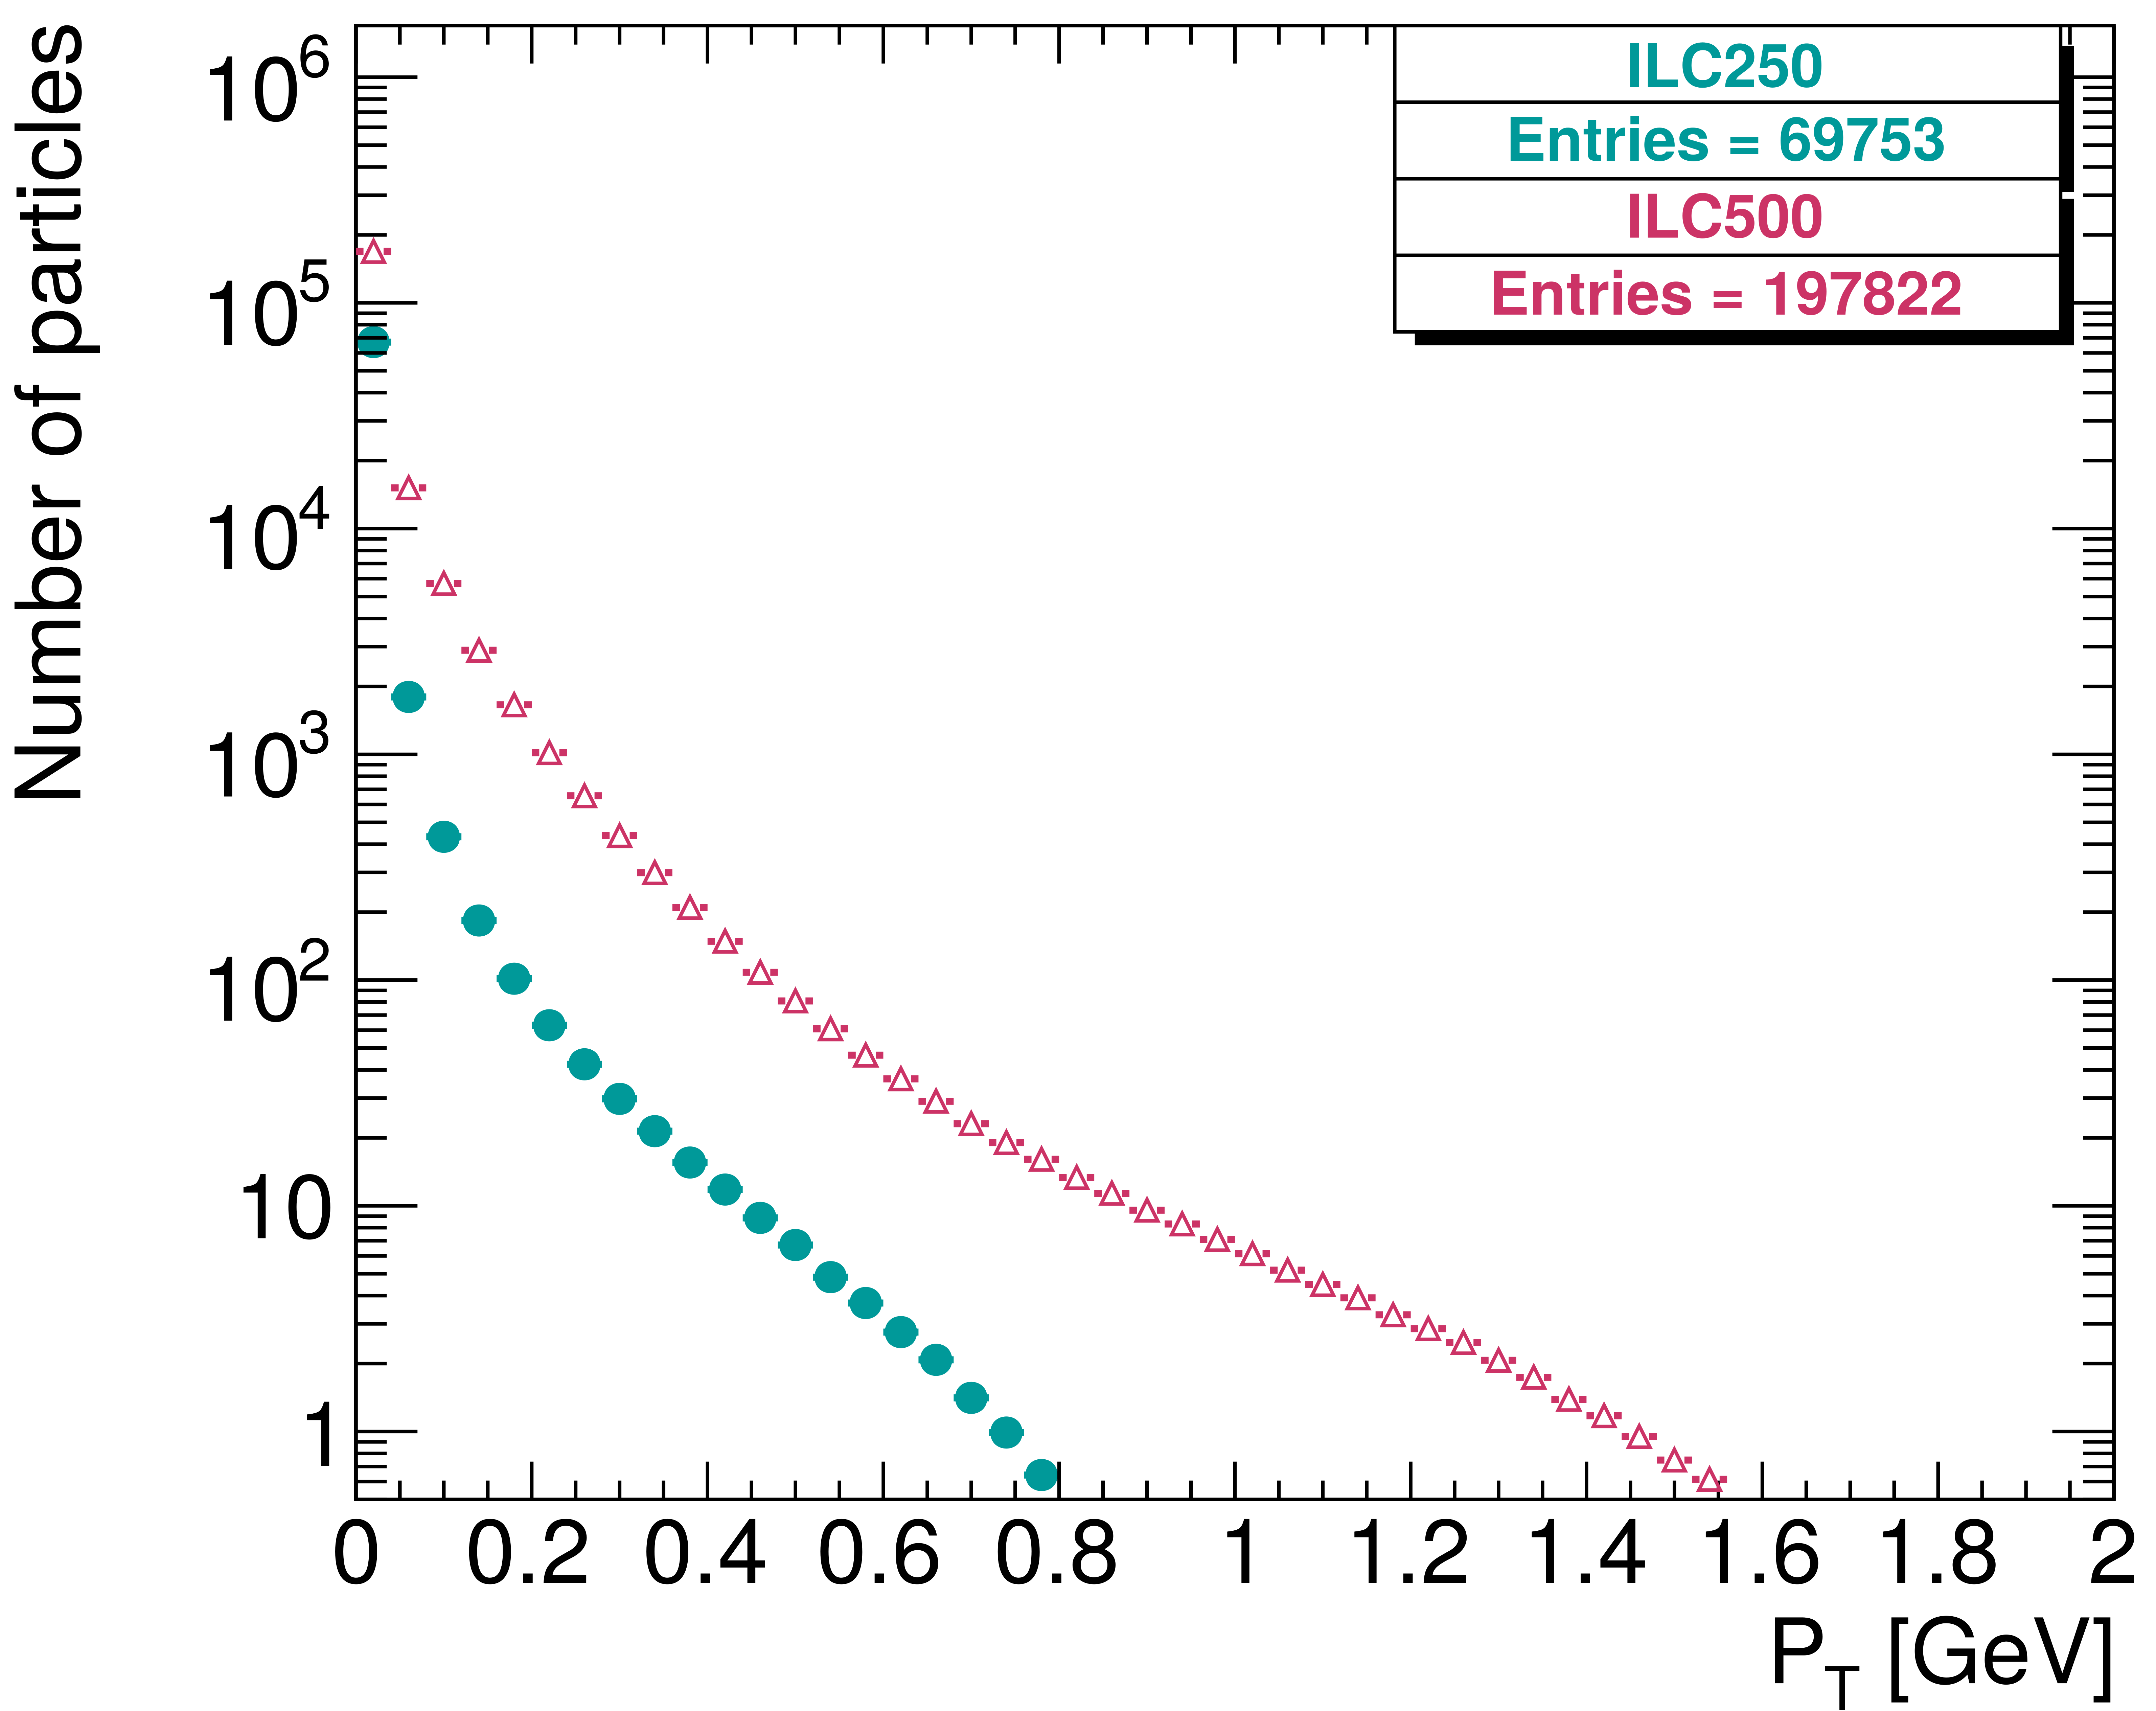
\includegraphics[width=0.96\textwidth]{Figures/Pairs/250_500_pairs_comparison_PT.png}
   \caption{Transverse momentum}
   \end{subfigure}
   \caption[Pair background momentum distributions]{Comparison of the pair background momentum distributions for the ILC at \SI{250}{\GeV} and \SI{250}{\GeV} center-of-mass energy, with the longitudinal momentum shown in Figure (a) and the transverse momentum in Figure (b).}
   \label{fig:PairBkg:Momentum}
 \end{figure}
\\Due to their low transverse momentum, the pairs are deflected on helical tracks in the magnetic field of the detector solenoid magnet.
An algorithm was written that calculates the helix tracks of the pair particles using their four-vectors. 
The track positions are computed from the radius of the helix, its center position and its pitch.
Figure~\ref{fig:helix_circle} shows schematically the projection of a helix onto the xy-plane.
The orientation of the helix is determined by the particle's charge.
The following assumptions were made for the algorithm:
The magnetic field in the proximity of the IP is homogeneous, with a field strength of \SI{5}{\tesla} for the \sid solenoid.
The particle momenta do not change in the region of interest for this analysis, because of which the helix radius is constant.
Any particle interaction with other particles or with matter is not taken into account.\\
\begin{figure}
    \centering
    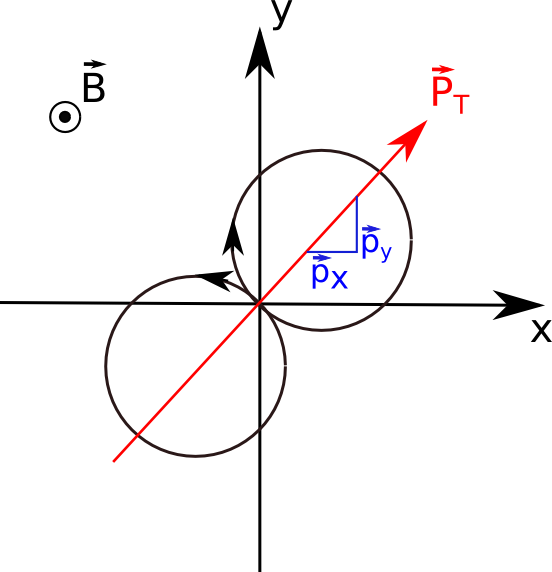
\includegraphics[width=0.3\textwidth]{Figures/Pairs/Helix_explanation.png}
    \caption[Schematic projection of the helix on the xy-plane]{
    This schematic shows the projection of a helix track onto the xy-plane, with the vector of the transverse momentum (P\textsubscript{T}) and the x- and y-momenta (p\textsubscript{x} and p\textsubscript{y}).
    Depending on the particle's charge, the direction of the rotation is either clockwise or anticlockwise.
    The center, the radius, and the orientation of the projected circle is dependent on the transverse momentum of the particle.
    }
    \label{fig:helix_circle}
\end{figure}
The pair tracks are then plotted using the helix track algorithm to calculate the position in x and y for a given position in z.
For the ILC stage at \SI{500}{\GeV}, the pair background was generated with \guineapig, and its density plotted in Figure~\ref{fig:PairBkg:Density} (a).
The density distribution of all the tracks shows a characteristic bell shape, with the highest density along the z-axis.
This is true, since the helix tracks originate at the IP, and their radii are small in comparison to their pitches due to the particles' momentum distribution.
The red solid lines represent the outline of the beam pipe inside the \sid detector.
Up to \SI{6.2}{\centi\meter} from the IP in the z-direction, where the beam pipe increases in width, the beam pipe radius is \SI{1.2}{\centi\meter}. \todo{English}
This is the point of closest approach to the pair background envelope.
Here, the pair helix tracks reach beyond the beam pipe.
\\As the bell shaped envelope is fully symmetrical in the positive and negative z-direction, as well as in the xz and yz-plane, the chosen view of the pair background envelopes will always be of the xz-plane in the positive z-direction.
 \begin{figure}
 \centering
  \begin{subfigure}[b]{0.49\textwidth}
   \centering
    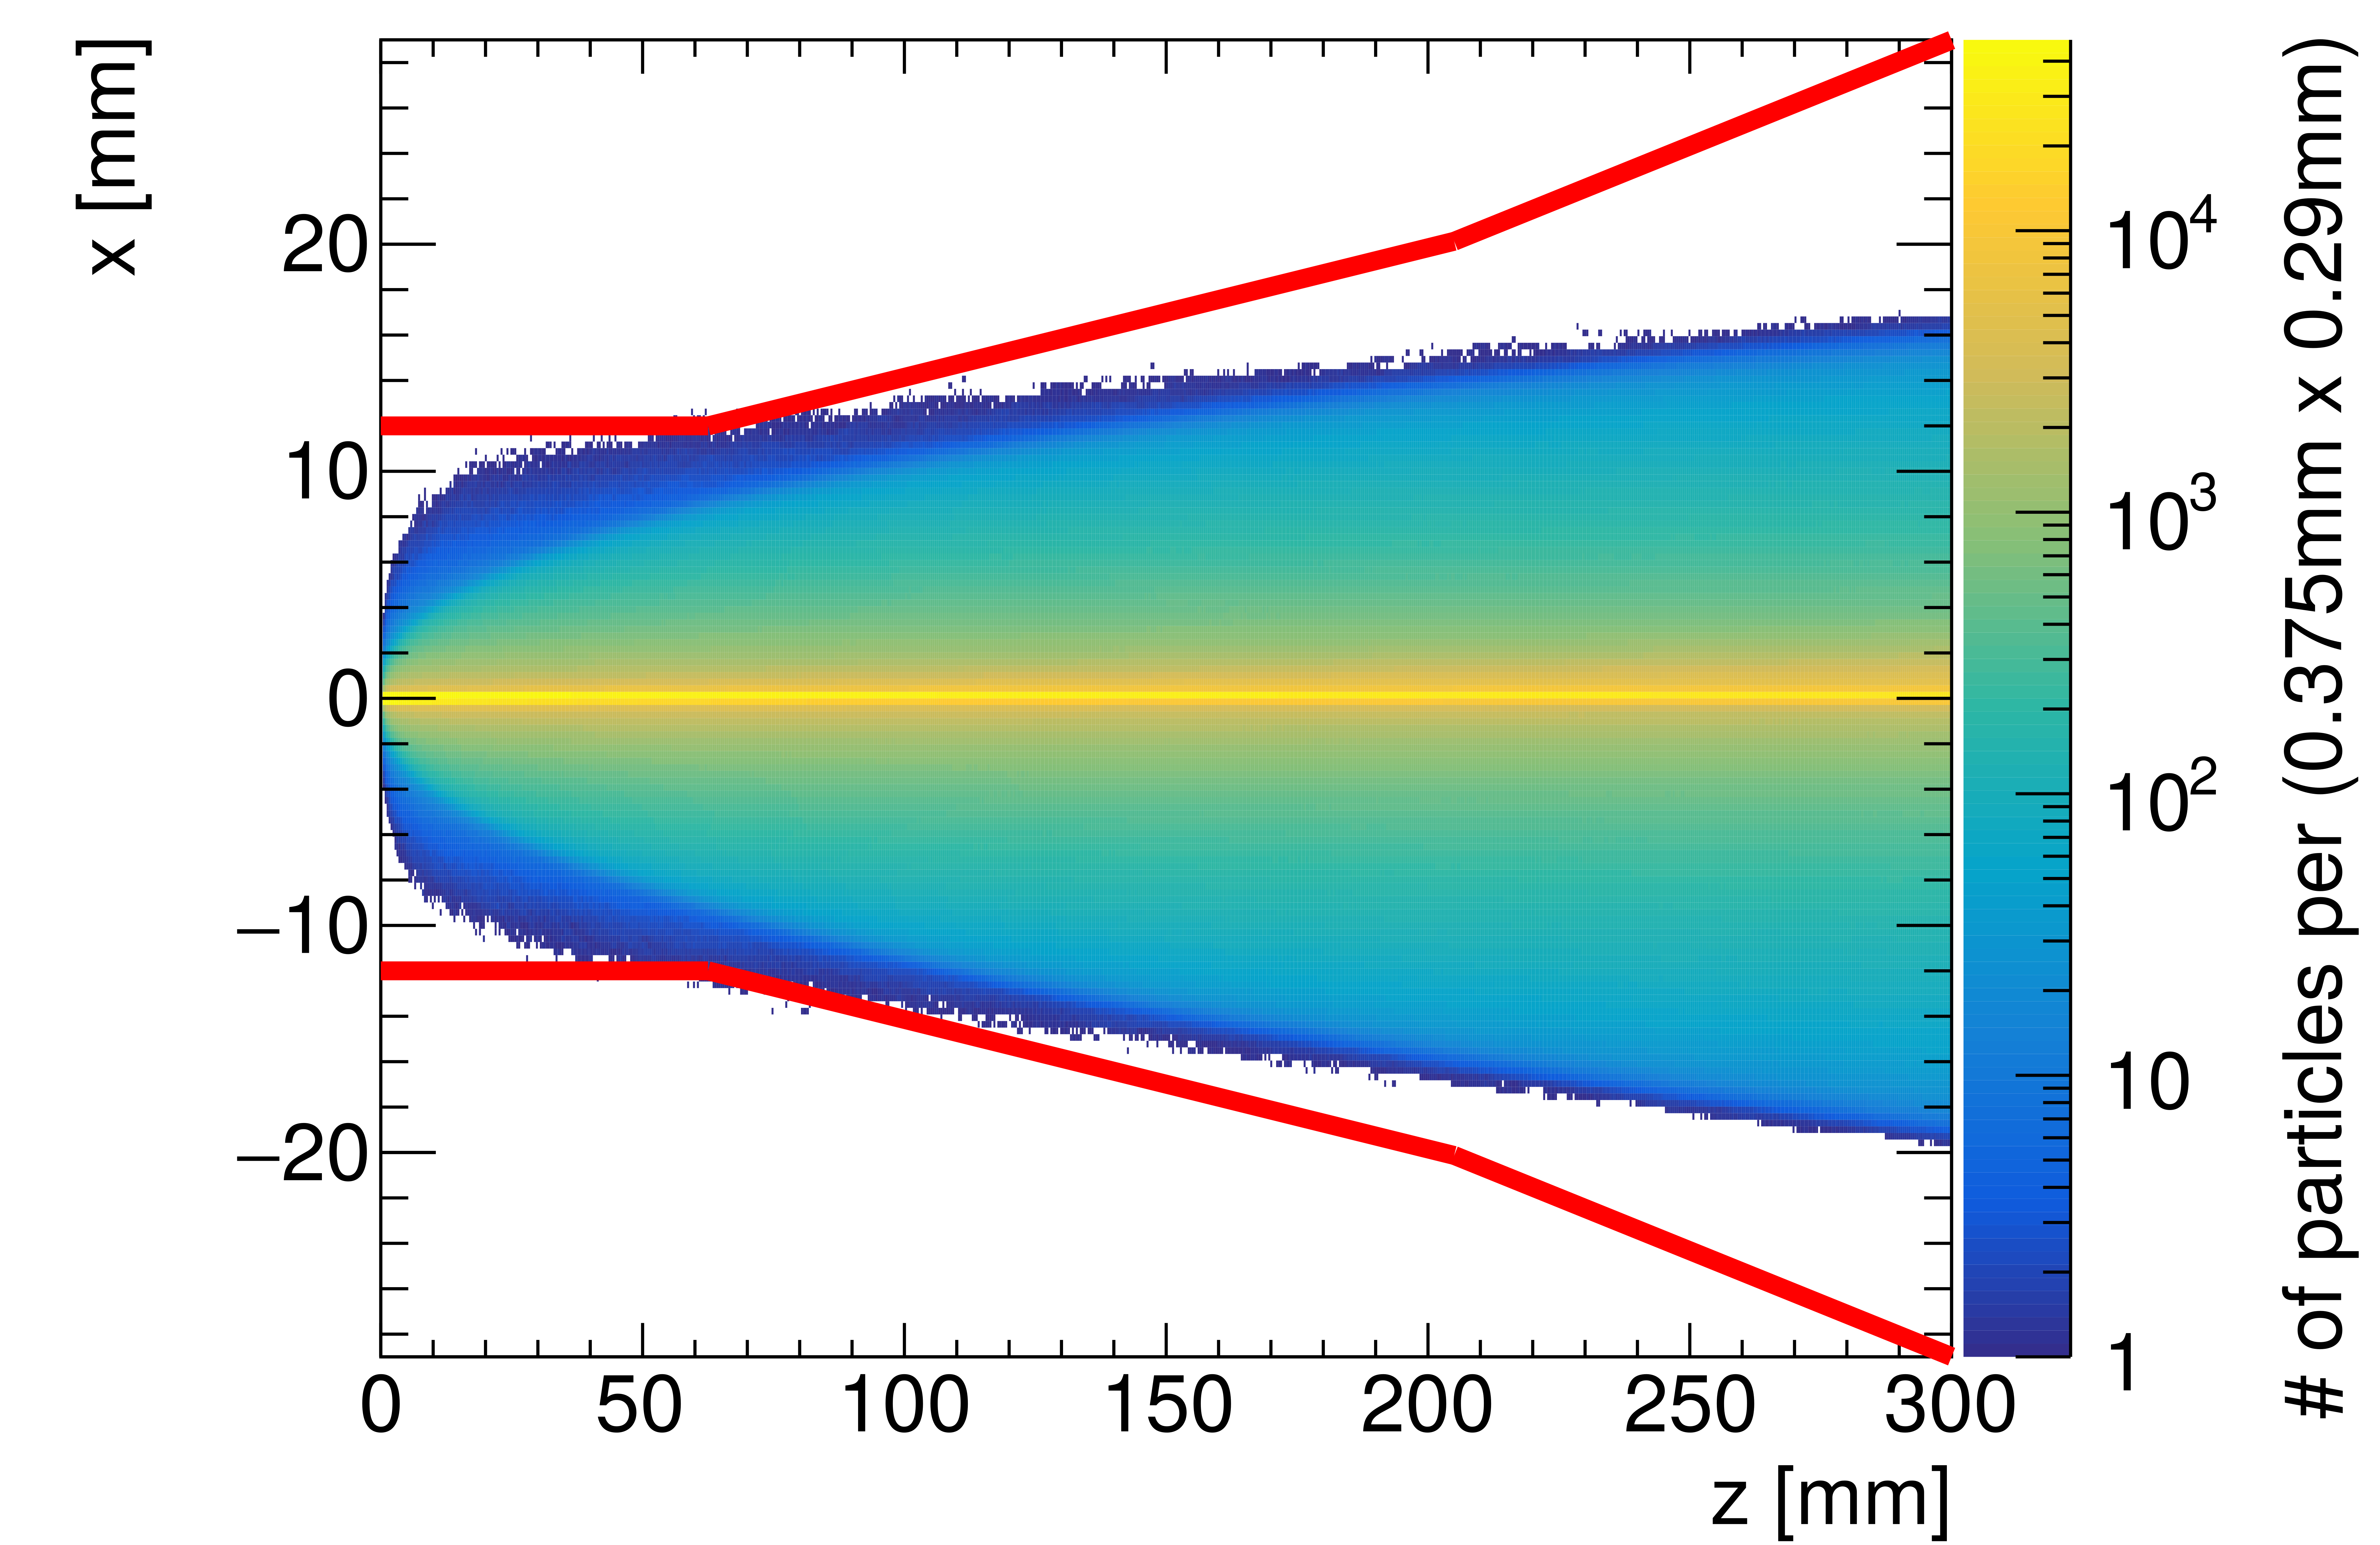
\includegraphics[width=\textwidth]{Figures/Pairs/Helix_tracks_xz_80bunches_500GeV_5T.png}
   \caption{Pair background density for the ILC500}
   \end{subfigure}
   \hfill
    \begin{subfigure}[b]{0.49\textwidth}
   \centering
    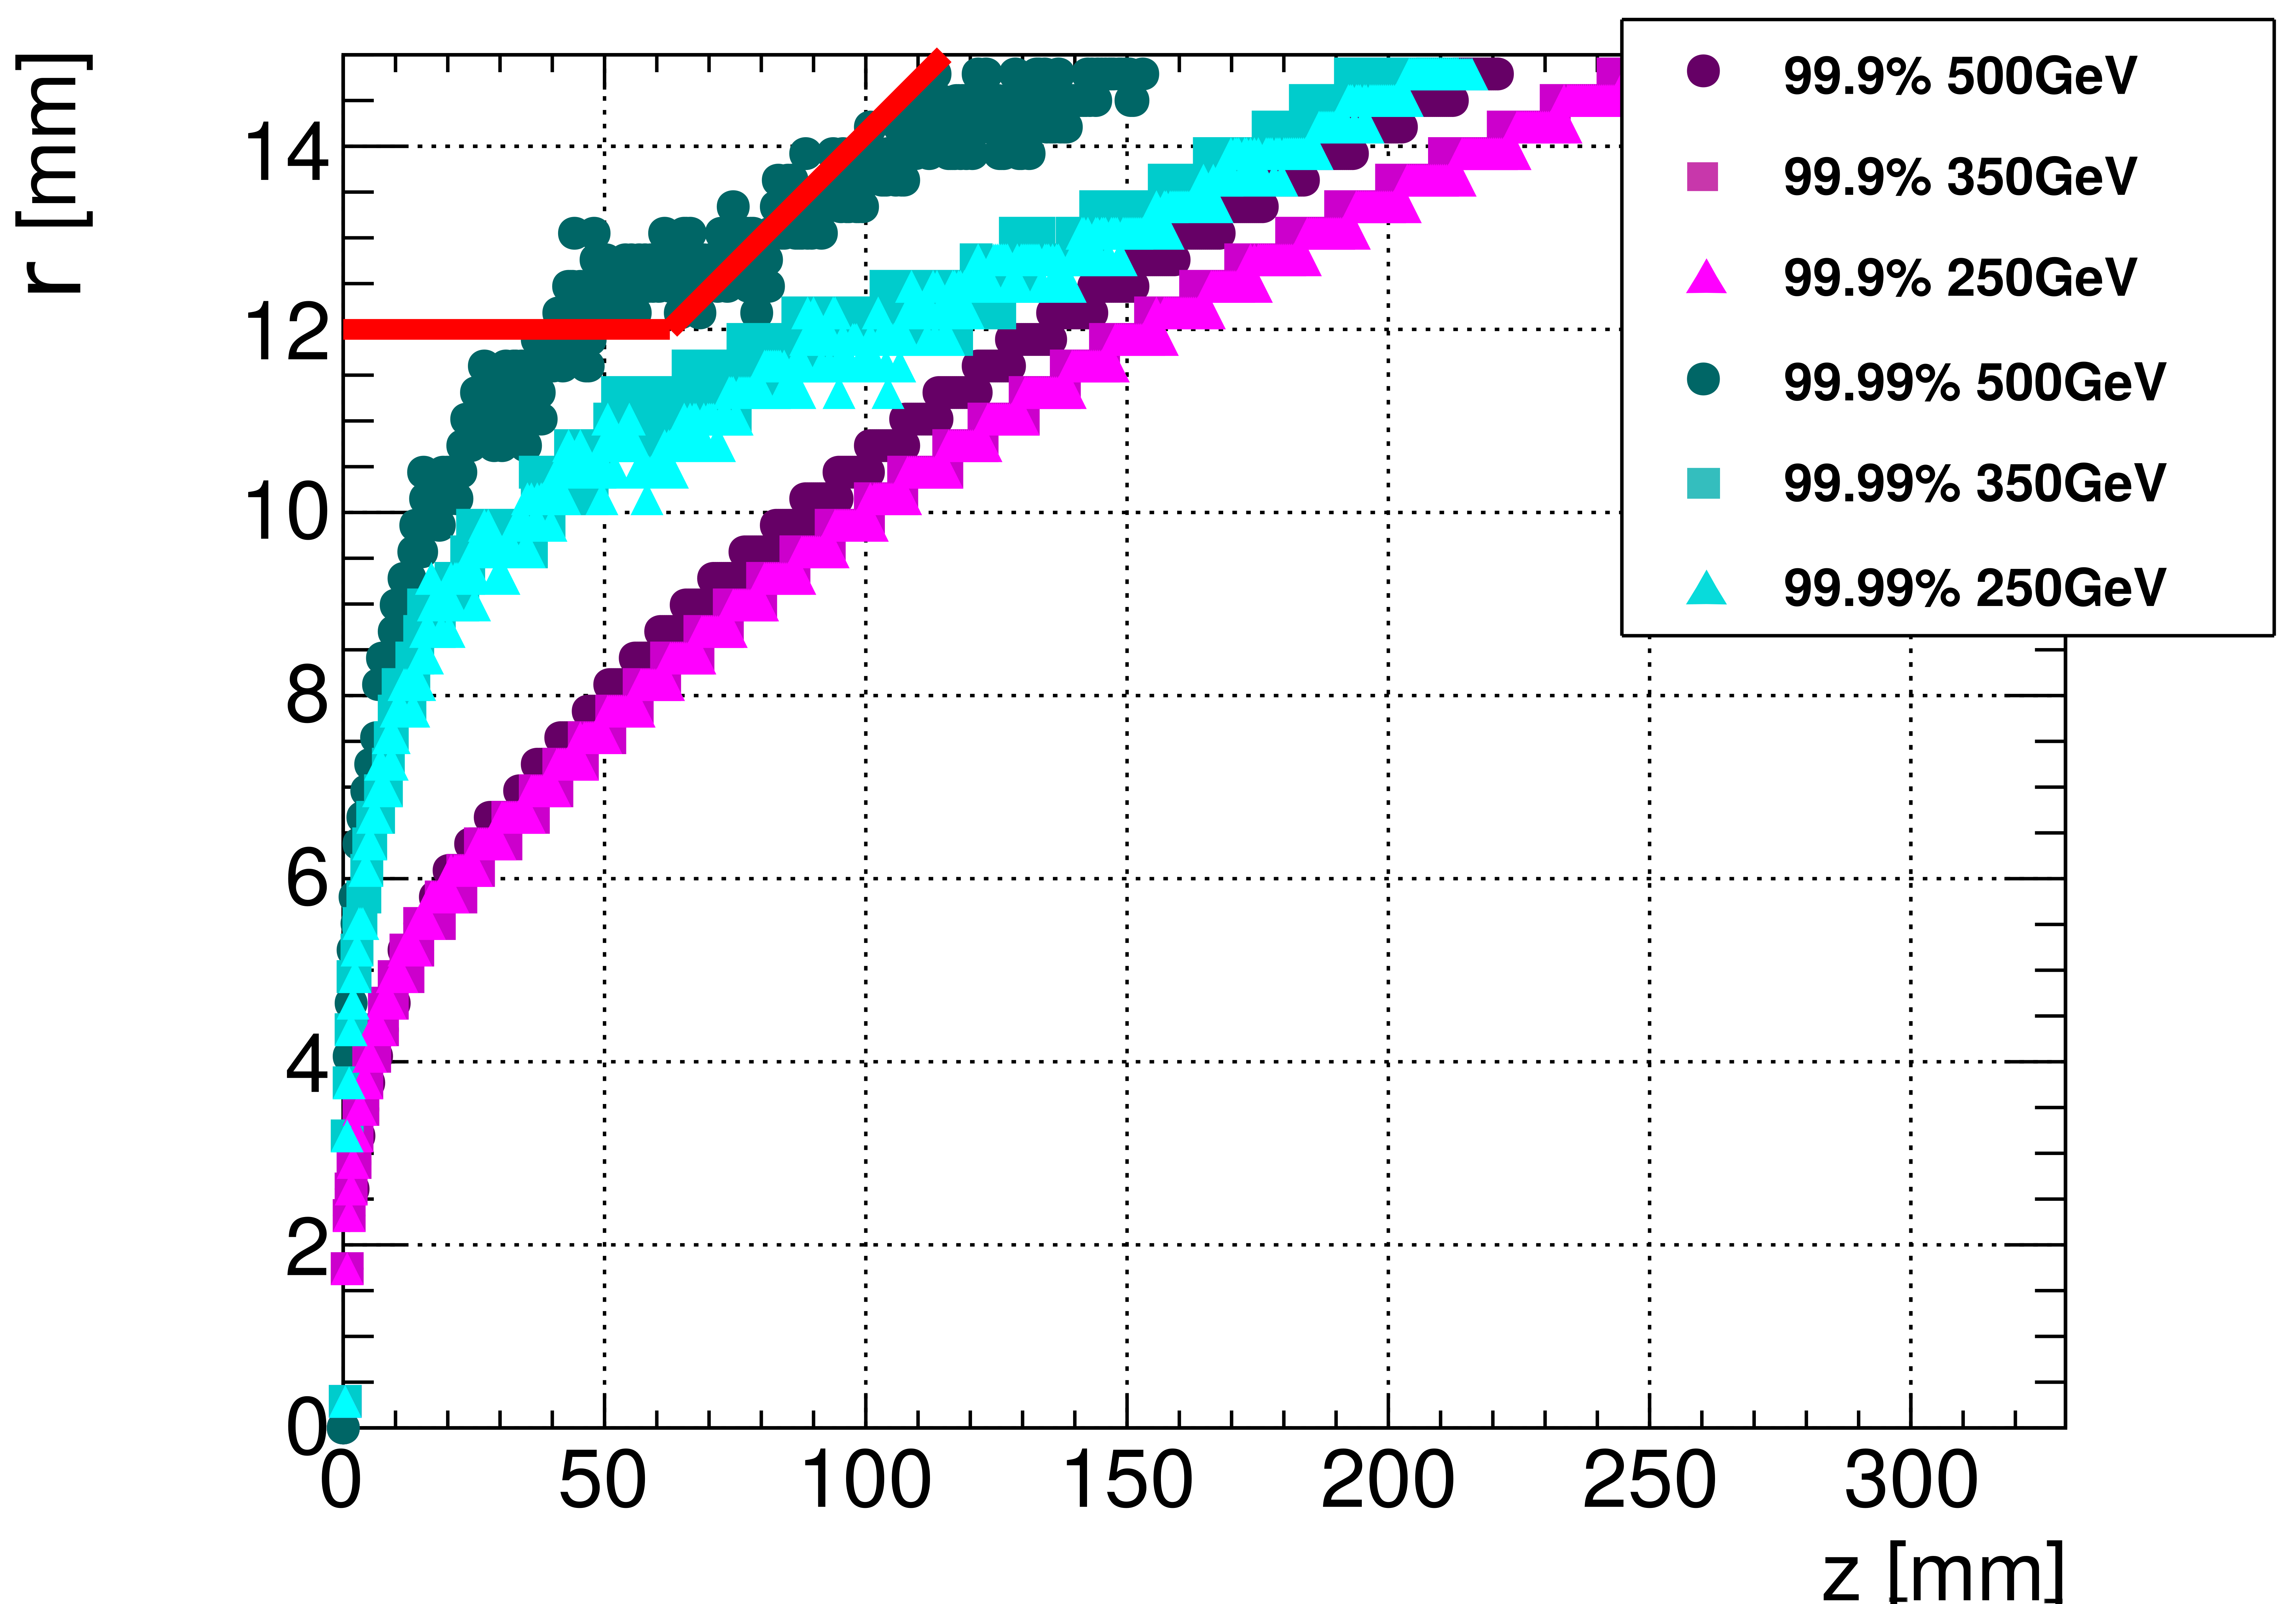
\includegraphics[width=\textwidth]{Figures/Pairs/HelixEnvelopes_COMPARISON_xz_500_350_250_comparison_EDITED_2.png}
   \caption{Pair background envelopes at different center-of-mass energies}
   \end{subfigure}
   \caption[Pair background density]{The figures display the pair background density in the xz-plane for one ILC bunch crossing.
   Figure (a) shows the complete track density distribution of the pairs at a center-of-mass energy of \SI[detect-all]{500}{\GeV}.
   The color scale shows the number of tracks per unit area.
   The red solid lines represent the outline of the beam pipe.
   \\In Figure (b), the density envelopes of three ILC stages are compared: at 250, 350, and \SI[detect-all]{500}{\GeV}.
   For that purpose, not the complete density distribution is plotted, but rather the envelopes containing either \SI[detect-all]{99.9}{\percent} or \SI[detect-all]{99.99}{\percent} of all tracks.
   }
   \label{fig:PairBkg:Density}
 \end{figure}
\\In order to compare the envelope shapes for different ILC beam parameters, Figure~\ref{fig:PairBkg:Density} (b) only shows the envelopes containing a certain fraction of all tracks.
In this way, it becomes apparent that for higher center-of-mass energies the width of the envelope increases due to the higher transverse momenta of the pairs.
At \SI{500}{\GeV}, the envelope containing \SI{99.99}{\percent} of all pair helix tracks crosses the beam pipe, extending towards the innermost layer of the \sid vertex detector, which has a radius of \SI{14}{\milli\meter}.
For lower center-of-mass energies, the envelopes stay well within the beam pipe radius.
The pair background simulation files for this comparison plot were generated with \guineapig as well, using the beam parameters of the three different baseline ILC stages~\cite[p. 11]{TDR1}.

\section{Impact of the pair background studies on ILC design choices}
\subsection{Pair background dependency on ILC beam parameters}
As explained in Section~\ref{ILC:layout:staging}, the first ILC stage will be at \SI{250}{\GeV} instead of the originally anticipated \SI{500}{\GeV}.
Due to this decision in 2017, efforts have been made to study a possible change in the baseline beam parameters for this stage in order to increase the luminosity from \num{8.2} to \SI{16.2e34}{\per\centi\meter\squared\per\second}~\cite{LCWS17_paper}. 
To this end, three alternative beam parameter sets have been suggested, which vary from the original baseline parameters in the emittance and the beta function values.
The values which differ are listed in Table~\ref{tab:ILC250_sets}.
For all alternative sets, the horizontal emittance $\epsilon_x$ is reduced. 
Additionally, the horizontal and vertical beta functions at the IP, $\beta^*_x$ and $\beta^*_y$, are changed for sets (B) and (C).
Since both the emittance and the beta function are dependencies of the beam size, they enter indirectly the Equation~\ref{eq:luminosity} for the beam luminosity.
\\On the other hand, a reduced horizontal emittance implies also an increase in the beam-beam interactions and in the pair background level.
For the process of deciding the new official beam parameter set, a study of the impact of this increased pair background on the \sid vertex detector performance was therefore a crucial step.
In the following, the simulation studies of the pair background for the four parameter schemes listed in Table~\ref{tab:ILC250_sets} are presented.
\begin{table}
\caption[New ILC250 beam parameters]{Changes between the baseline and alternative beam parameter sets for the ILC stage at \SI[detect-all]{250}{\GeV}~\cite{LCWS17_paper}.
The highlighted parameter set (A) was chosen to be the new official scheme for the ILC250.
A full set of the baseline beam parameters can be found in~\cite[p. 11]{TDR1}.}
\label{tab:ILC250_sets}
\centering
\begin{tabularx}{0.48\textwidth}{c|ccc}
\hline\hline
\textbf{ILC250 sets} & $\epsilon_x$ (\si{\micro\meter}) & $\beta^*_x$ (\si{\milli\meter}) & $\beta^*_y$ (\si{\milli\meter})\\
\hline
 Baseline & 10.0 & 13.0 & 0.41\\
\rowcolor{Gray} (A) & 5.0 & 13.0 & 0.41\\
 (B) & 5.0 & 9.19 & 0.41\\
 (C) & 5.0 & 9.19 & 0.58\\
\hline\hline
\end{tabularx}
\end{table}

\begin{figure}
\centering
\begin{subfigure}[t]{0.49\textwidth}
\centering
\includegraphics[width=\textwidth]{Figures/Pairs/Helix_tracks_xz_100bunches_250GeV_5T_DanielJeans-1.jpg}
\caption{ILC250 set (TDR)}
\end{subfigure}
\hspace*{0.08cm}
\begin{subfigure}[t]{0.49\textwidth}
\centering
\includegraphics[width=\textwidth]{Figures/Pairs/Helix_tracks_xz_80bunches_250GeV_5T_Reduced_Emittance_x-1.jpg}
\caption{ILC250 set (A)}
\end{subfigure}
\\
\begin{subfigure}[t]{0.49\textwidth}
\centering
\includegraphics[width=\textwidth]{Figures/Pairs/Helix_tracks_xz_50bunches_250GeV_5T_Reduced_Emittance_x_Reduced_Beta_x-1.jpg}
\caption{ILC250 set (B)}
\end{subfigure}
\hspace*{0.08cm}
\begin{subfigure}[t]{0.49\textwidth}
\centering
\includegraphics[width=\textwidth]{Figures/Pairs/Helix_tracks_xz_50bunches_250GeV_5T_Reduced_Emittance_x_Reduced_Beta_x_Increased_Beta_y-1.jpg}
\caption{ILC250 set (C)}
\end{subfigure}
\caption[Pair background density for the proposed ILC250 beam parameter sets]{Pair background density for the four ILC250 beam parameter sets listed in Table~\ref{tab:ILC250_sets} per bunch crossing. 
The color scale shows the number of tracks per unit area.
The beam pipe is represented by the red solid lines.}
\label{fig:PairBkg:ILC250_Envelopes}
\end{figure}
The pair background density plots for the four schemes are shown in Figure~\ref{fig:PairBkg:ILC250_Envelopes}.
The width of the envelopes for the new proposed parameter sets (A), (B), and (C) is significantly increased compared to the baseline set (TDR).
Again, for the direct comparison of the pair background density from different ILC running scenarios, the two-dimensional plots of the track densities are not ideal.
Instead, Figure~\ref{fig:PairBkg:Density_Projection} shows a projection of the number of pair particles along the x-axis at the z-position of the first beam pipe kink, where the beam pipe radius increases.
It therefore holds more information than the previous plots: the envelope width in x at the specified z-position, and the number of particles at any given x value, for all beam parameter sets.
\\First of all, it becomes clear that the number of pair particles does indeed increase for the new beam parameter sets due to the enhanced beam-beam interactions.
Compared to the baseline set (the TDR set), the number of particles in set (A) is increased by a factor of 2-3, and by a factor of 6-7 in sets (B) and (C).
Furthermore, the so-called pair edge is clearly visible as the rapid decrease in density at around \SI{9}{\milli\meter} from the center.
Since the pink vertical lines in the picture represent the beam pipe, the pair edge is well contained within the beam pipe.
Nevertheless, there are background levels observed outside the beam pipe, extending beyond the vertex detector layers.
These levels, however, are below 5 particles per x-position.
With the track information across the five layers of the vertex detector, the vertices of particles created in the bunch collision can be reconstructed.
By populating the innermost layers with background particles, the reconstruction efficiency inevitably declines.
The occupancy from the pair background therefore has to be studied with respect to its impact on the detector performance.
\begin{figure}
    \centering
    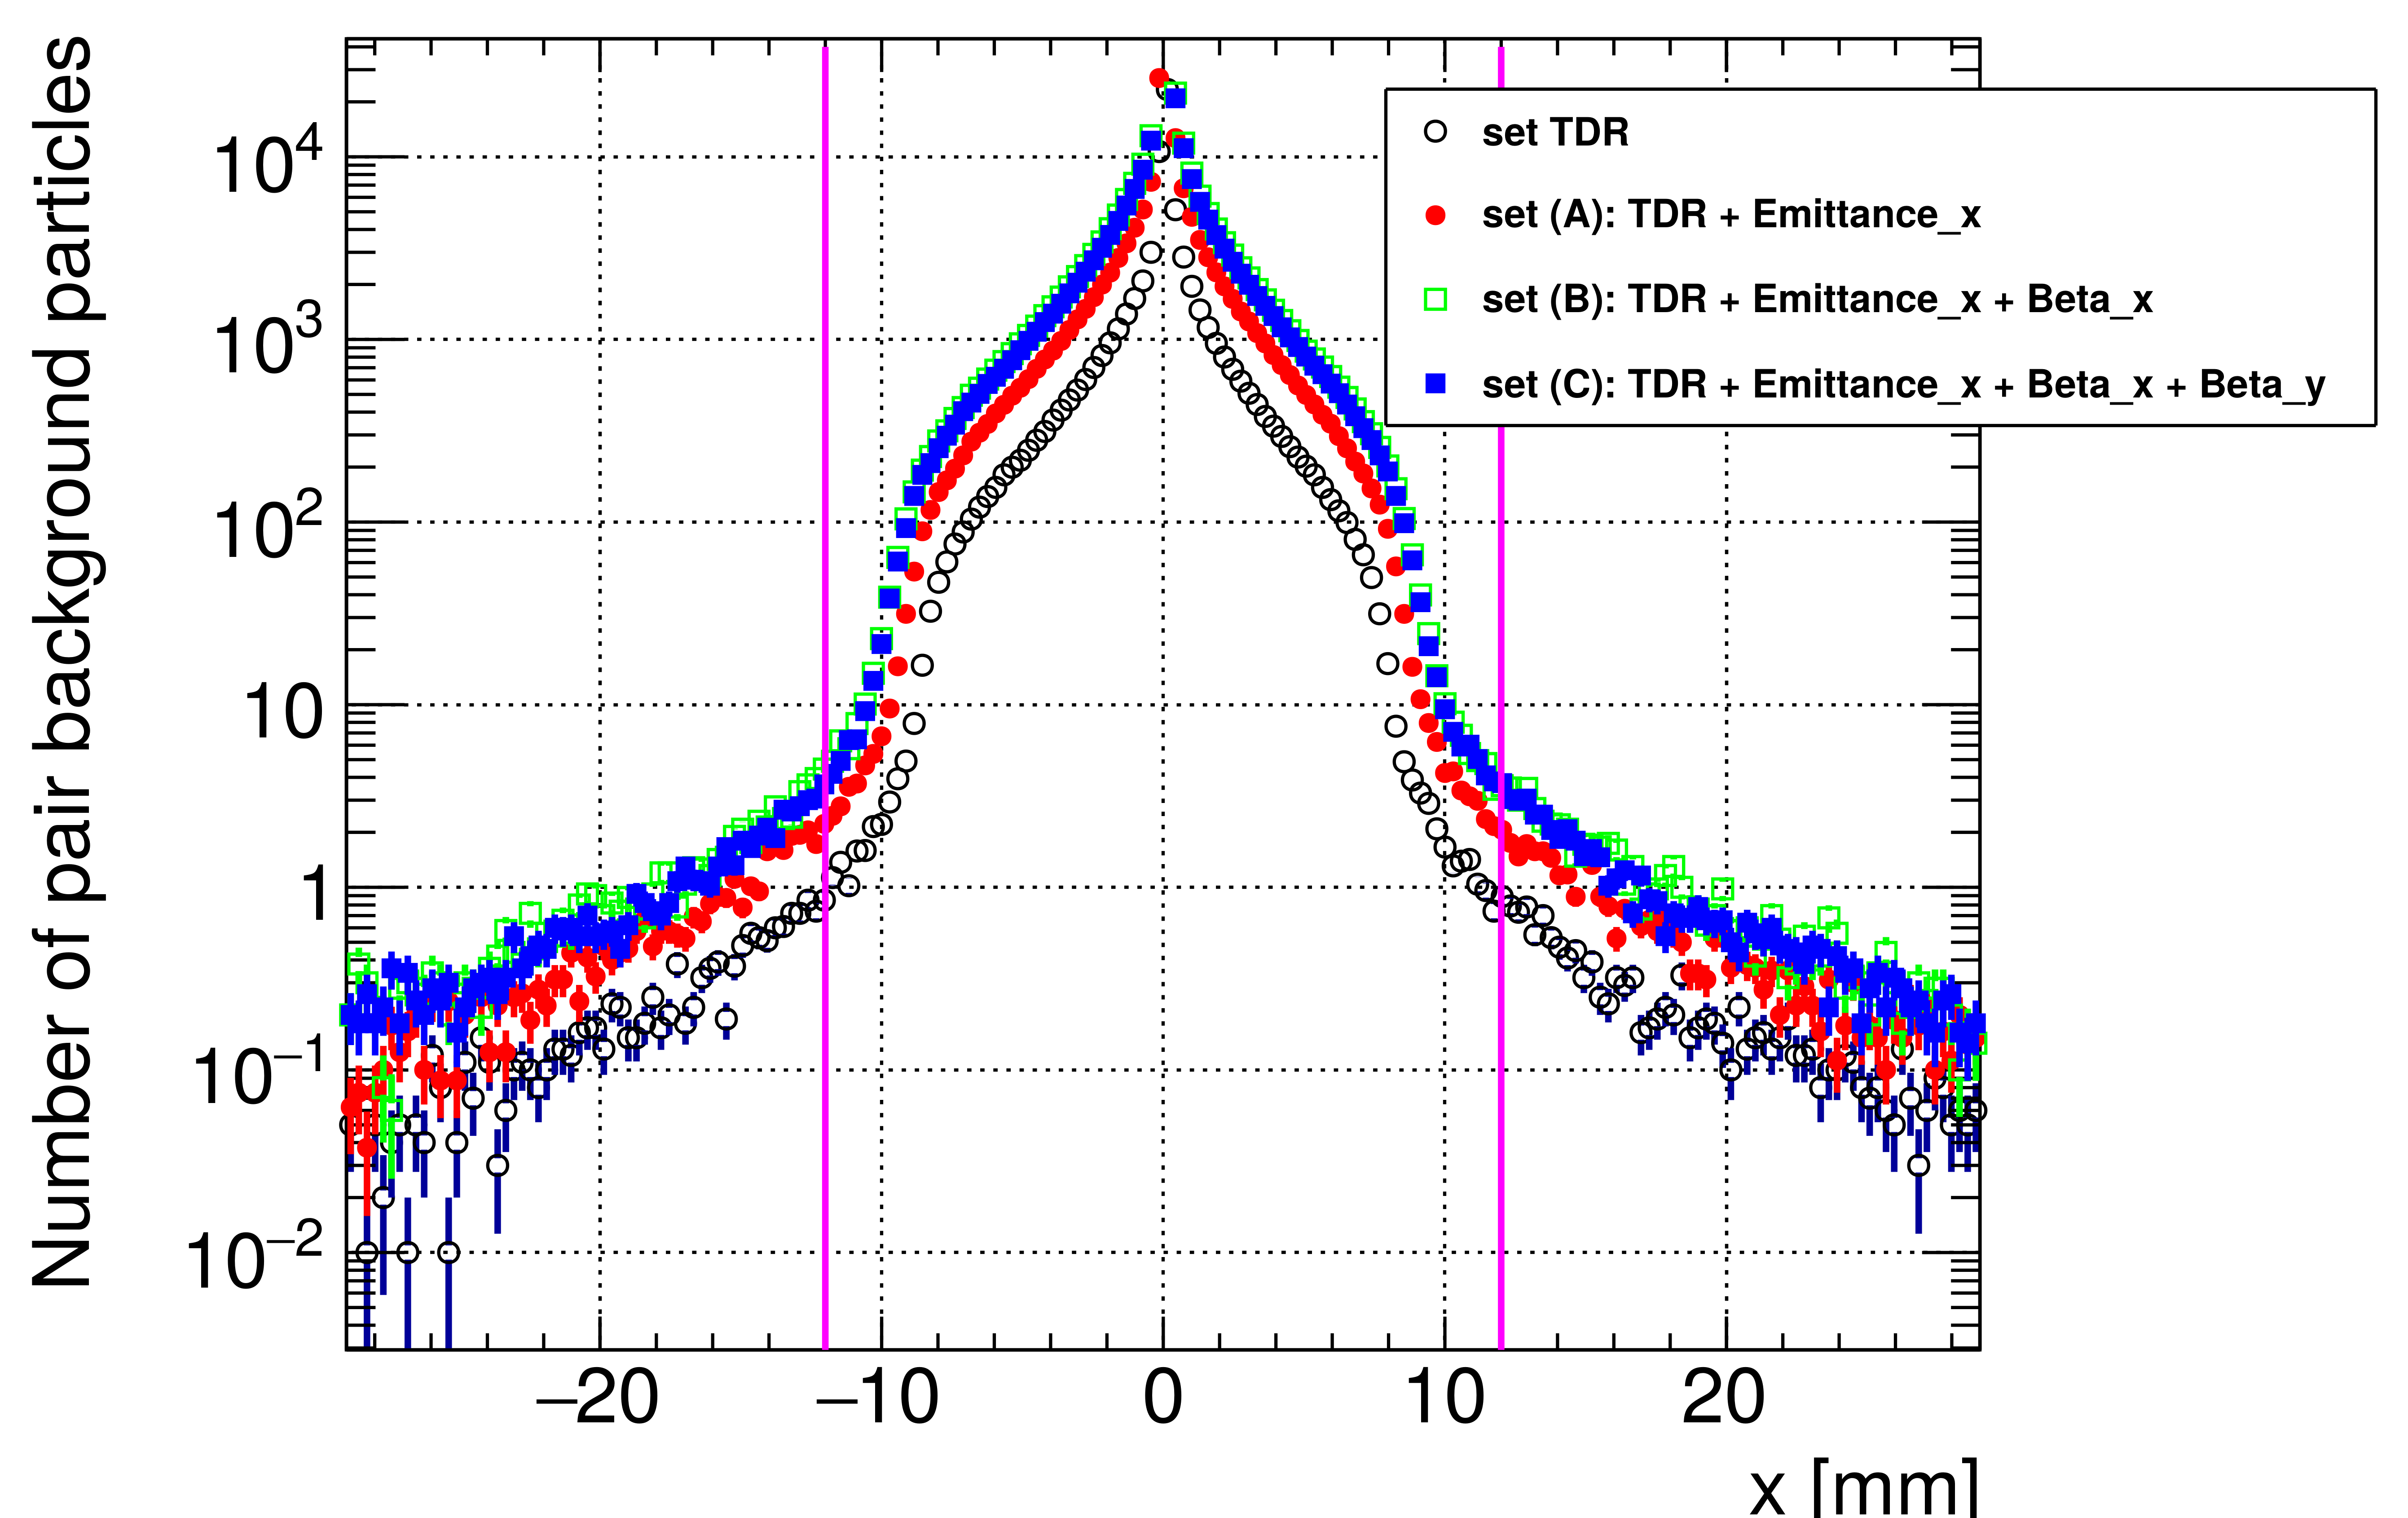
\includegraphics[width=0.7\textwidth]{Figures/Pairs/HelixEnvelope_Projection_Comparison_250GeV_parametersets_LEG.png}
    \caption[Pair background density projection for different ILC250 beam parameter sets]{
    Comparison of the pair background density projection for the four different ILC250 beam parameter sets.
    The plot shows the projected number of pairs along the x-axis for z = \SI[detect-all]{62}{\milli\meter}, which is the z-position of the first beam pipe kink.
    The pink vertical lines represent the beam pipe radius at this z-position.
    }
    \label{fig:PairBkg:Density_Projection}
\end{figure}

\subsection{Occupancy studies and buffer depth}
\label{PairBkg:occupancy}
For the vertex detector occupancy studies, the number of hits of every detector cell is counted and translated into an occupancy.
In the following occupancy plots, the number of cells receiving a certain number of hits can be determined.
Knowing that a detector sensor can only store up to a specific number of hits (the so-called buffer depth), the number of ``dead'' cells can then be calculated.
A cell is defined to be dead when the buffer of its sensor is already completely filled, and no further hits can be stored.
This is especially important as the detectors for the ILC will read out their buffers only after every bunch train (\num{1312} bunch crossings).
In order to guarantee that cell buffers are not filled only by background hits, a balance has to be found between a sufficient buffer depth and low background levels, depending on the design of the accelerator and the detectors.
In \sid, a guideline for an acceptable occupancy for background events is that the sum of all cells with a number of hits greater than or equal to the buffer depth should not exceed \SI{0.01}{\percent} (\num{e-4} of all cells). 
\\The occupancy for all vertex detector layers combined after a full bunch train are shown for the barrel in Figure~\ref{fig:PairBkg:ILC250_Occupancy} (a) and for the endcaps in Figure~\ref{fig:PairBkg:ILC250_Occupancy} (c).
For producing these plots, pair background simulation files for \num{1312} bunch crossings have been generated with \guineapig, and the number of hits were counted for each cell, summed up over the full bunch train.
A cell size of \SI{20}{\micro\meter}\,x\,\SI{20}{\micro\meter} has been assumed for these calculations.
Plotting the number of cells with a certain amount of hits, and normalizing these numbers by the total number of cells in all vertex detector layers, results in Figure~\ref{fig:PairBkg:ILC250_Occupancy} (a) and (c).
It can be directly seen which percentage of all cells get hit a certain number of times.
Comparing the results from the four different ILC250 beam parameter sets for the vertex detector barrel and endcaps, the occupancy of set (A) is raised by a factor of 3 with respect to the baseline set (TDR).
For set (B) and (C), the occupancy is increased by a factor of about 6.
In the vertex detector endcaps, the occupancy is in general higher than in the barrel, leading to the fact that cells are hit up to 50 times compared to 40 times for the barrel.
The reason for this is that the pair background envelopes widen towards the endcaps, as can be seen from the density plots in Figure~\ref{fig:PairBkg:ILC250_Envelopes}.
\\As the readout design for the vertex detector is not yet decided, optimizations based on simulation recommendations can still be made.
In Figure~\ref{fig:PairBkg:ILC250_Occupancy} (b) and (d), the number of dead cells are therefore plotted as a function of the assumed buffer depth of the sensors.
The buffer depth states how many hits a sensor can store, before the according cell is blind to any further hits.
The buffer depth is in principle a free choice in the detector development phase.
The more buffers a sensor has, the more hits can be stored.
This does however not come for free, since sensors with a large number of buffers, or with dynamically allocatable buffers, have a higher power consumption.
The additional electric circuits that are required to meet the higher demand, and with it the supplementary cooling, lead to a larger material budget, which is not desirable for the vertex detector.
A compromise has to be made between necessary buffers and a manageable material budget.  
\\In the current detector design, the sensors have a buffer depth of four. 
The number of the dead cells is calculated from the occupancy plots in Figure~\ref{fig:PairBkg:ILC250_Occupancy} (a) and (c), and depends on the buffer depth.
For this buffer depth, Figure~\ref{fig:PairBkg:ILC250_Occupancy} (b) shows that for set (A) \num{8e-6} of all cells in all vertex detector barrel layers are dead, which is an increase with respect to the baseline set of a factor of four.
Nevertheless, \num{8e-6} is more than one order of magnitude below the critical limit of \num{e-4} of all cells.
\\As mentioned above, the occupancy in the endcaps is higher, leading to a larger ratio of dead cells.
For the vertex detector endcaps, the number of dead cells for a buffer depth of four reaches the critical limit for sets (B) and (C) (see Figure~\ref{fig:PairBkg:ILC250_Occupancy} (d)).
The ratio for set (A) is still below the critical limit with about \num{4.2e-5}.\\
 \begin{figure}
 \centering
  \begin{subfigure}[b]{0.49\textwidth}
   \centering
    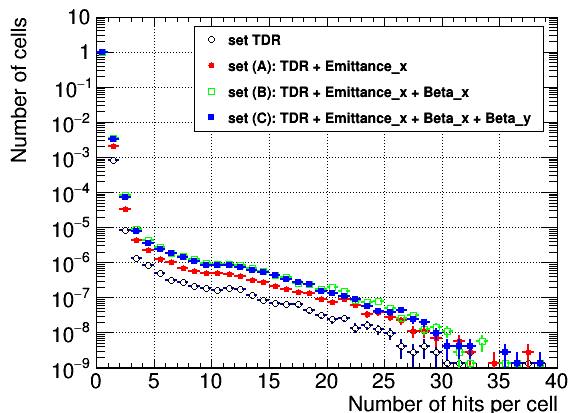
\includegraphics[width=\textwidth]{Figures/Pairs/Occupancy_Comparison_All_layers_wrt_cells_ILC250_Comparison_ALL_SETS_5T_w_antiDiD_LEG.png}
   \caption{Vertex detector \textbf{barrel}, normalized occupancy}
   \end{subfigure}
   \hfill
    \begin{subfigure}[b]{0.49\textwidth}
   \centering
    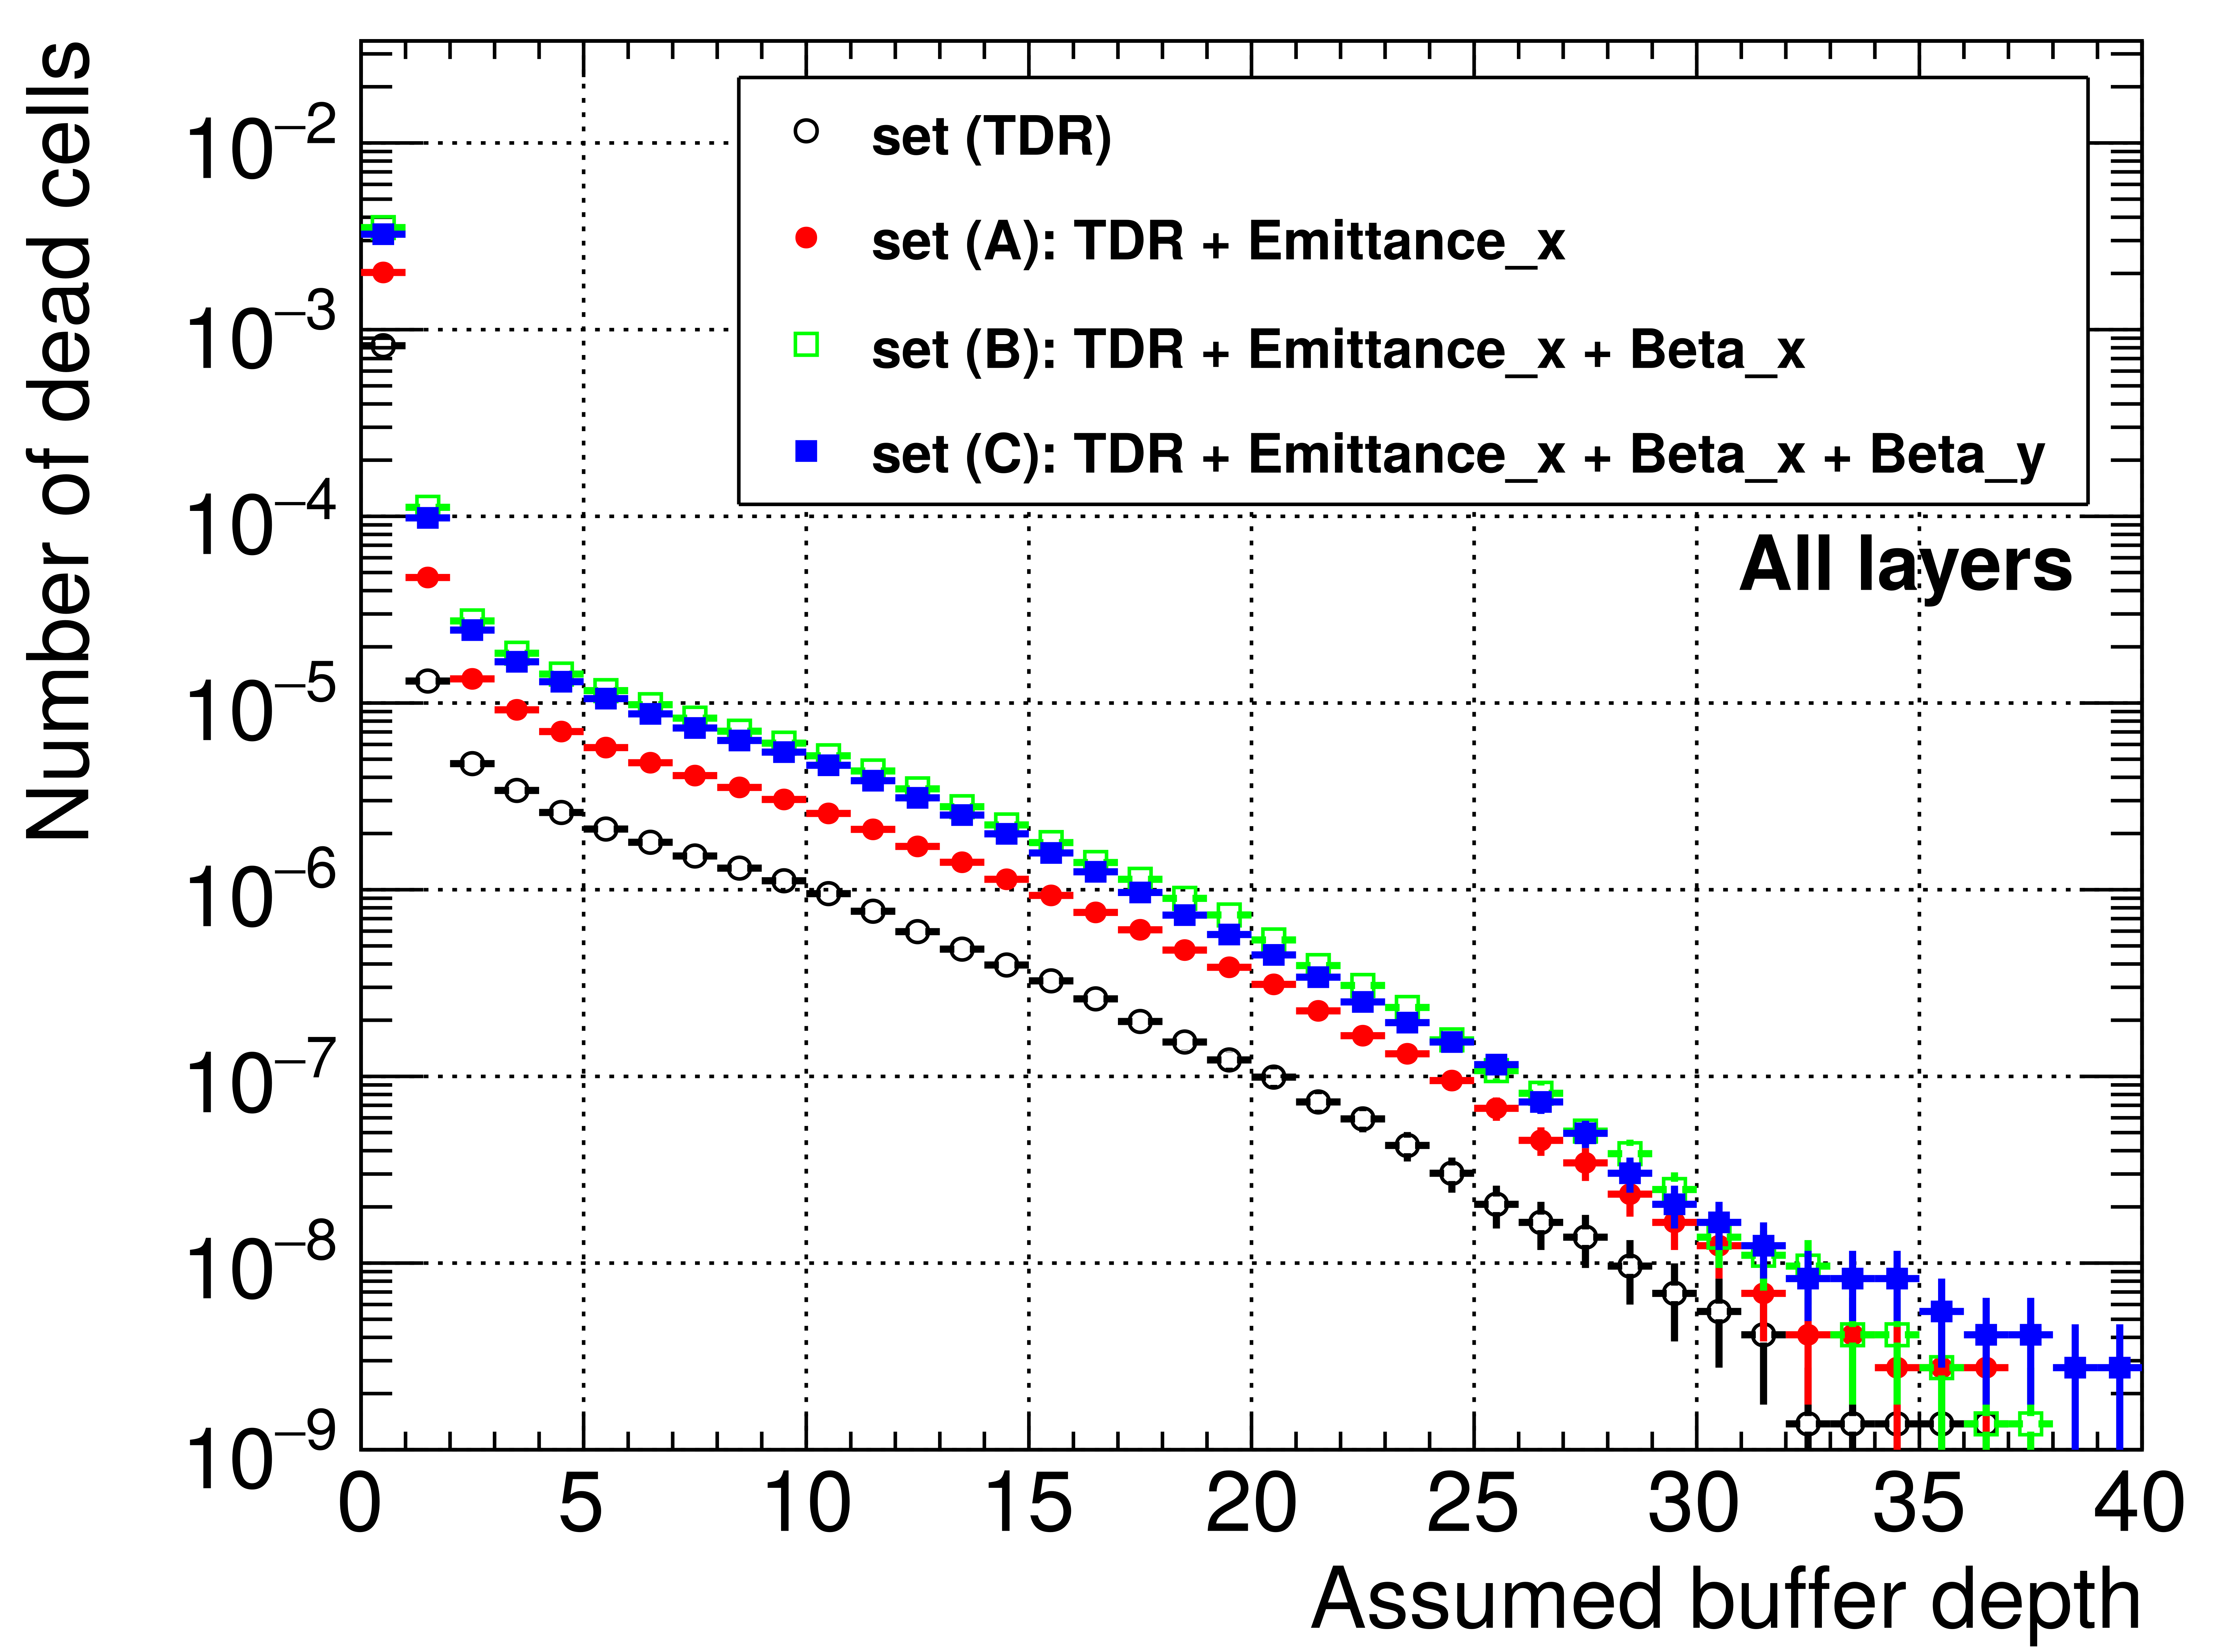
\includegraphics[width=\textwidth]{Figures/Pairs/Occupancy_Comparison_All_layers_deadcells_ILC250_Comparison_ALL_SETS_5T_w_antiDiD_LEG.png}
   \caption{Vertex detector \textbf{barrel}, ratio of dead cells}
   \end{subfigure}\\
  \begin{subfigure}[b]{0.49\textwidth}
   \centering
    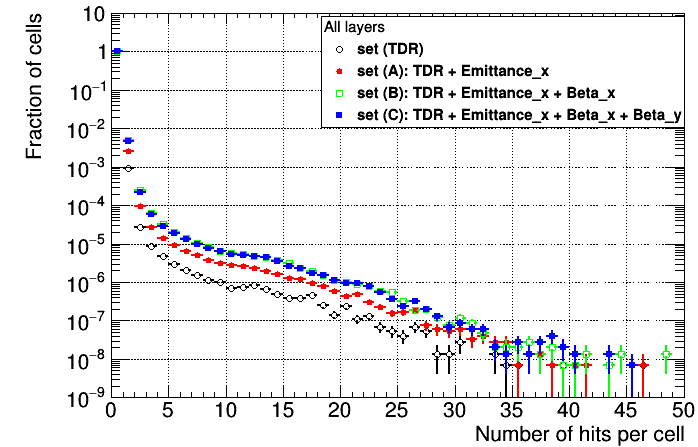
\includegraphics[width=\textwidth]{Figures/Pairs/Occupancy_Comparison_All_layers_wrt_cells_ILC250_ALL_SETS_5T_w_antiDiD_SiVertexEndcap.png}
   \caption{Vertex detector \textbf{endcaps}, normalized occupancy}
   \end{subfigure}
   \hfill
    \begin{subfigure}[b]{0.49\textwidth}
   \centering
    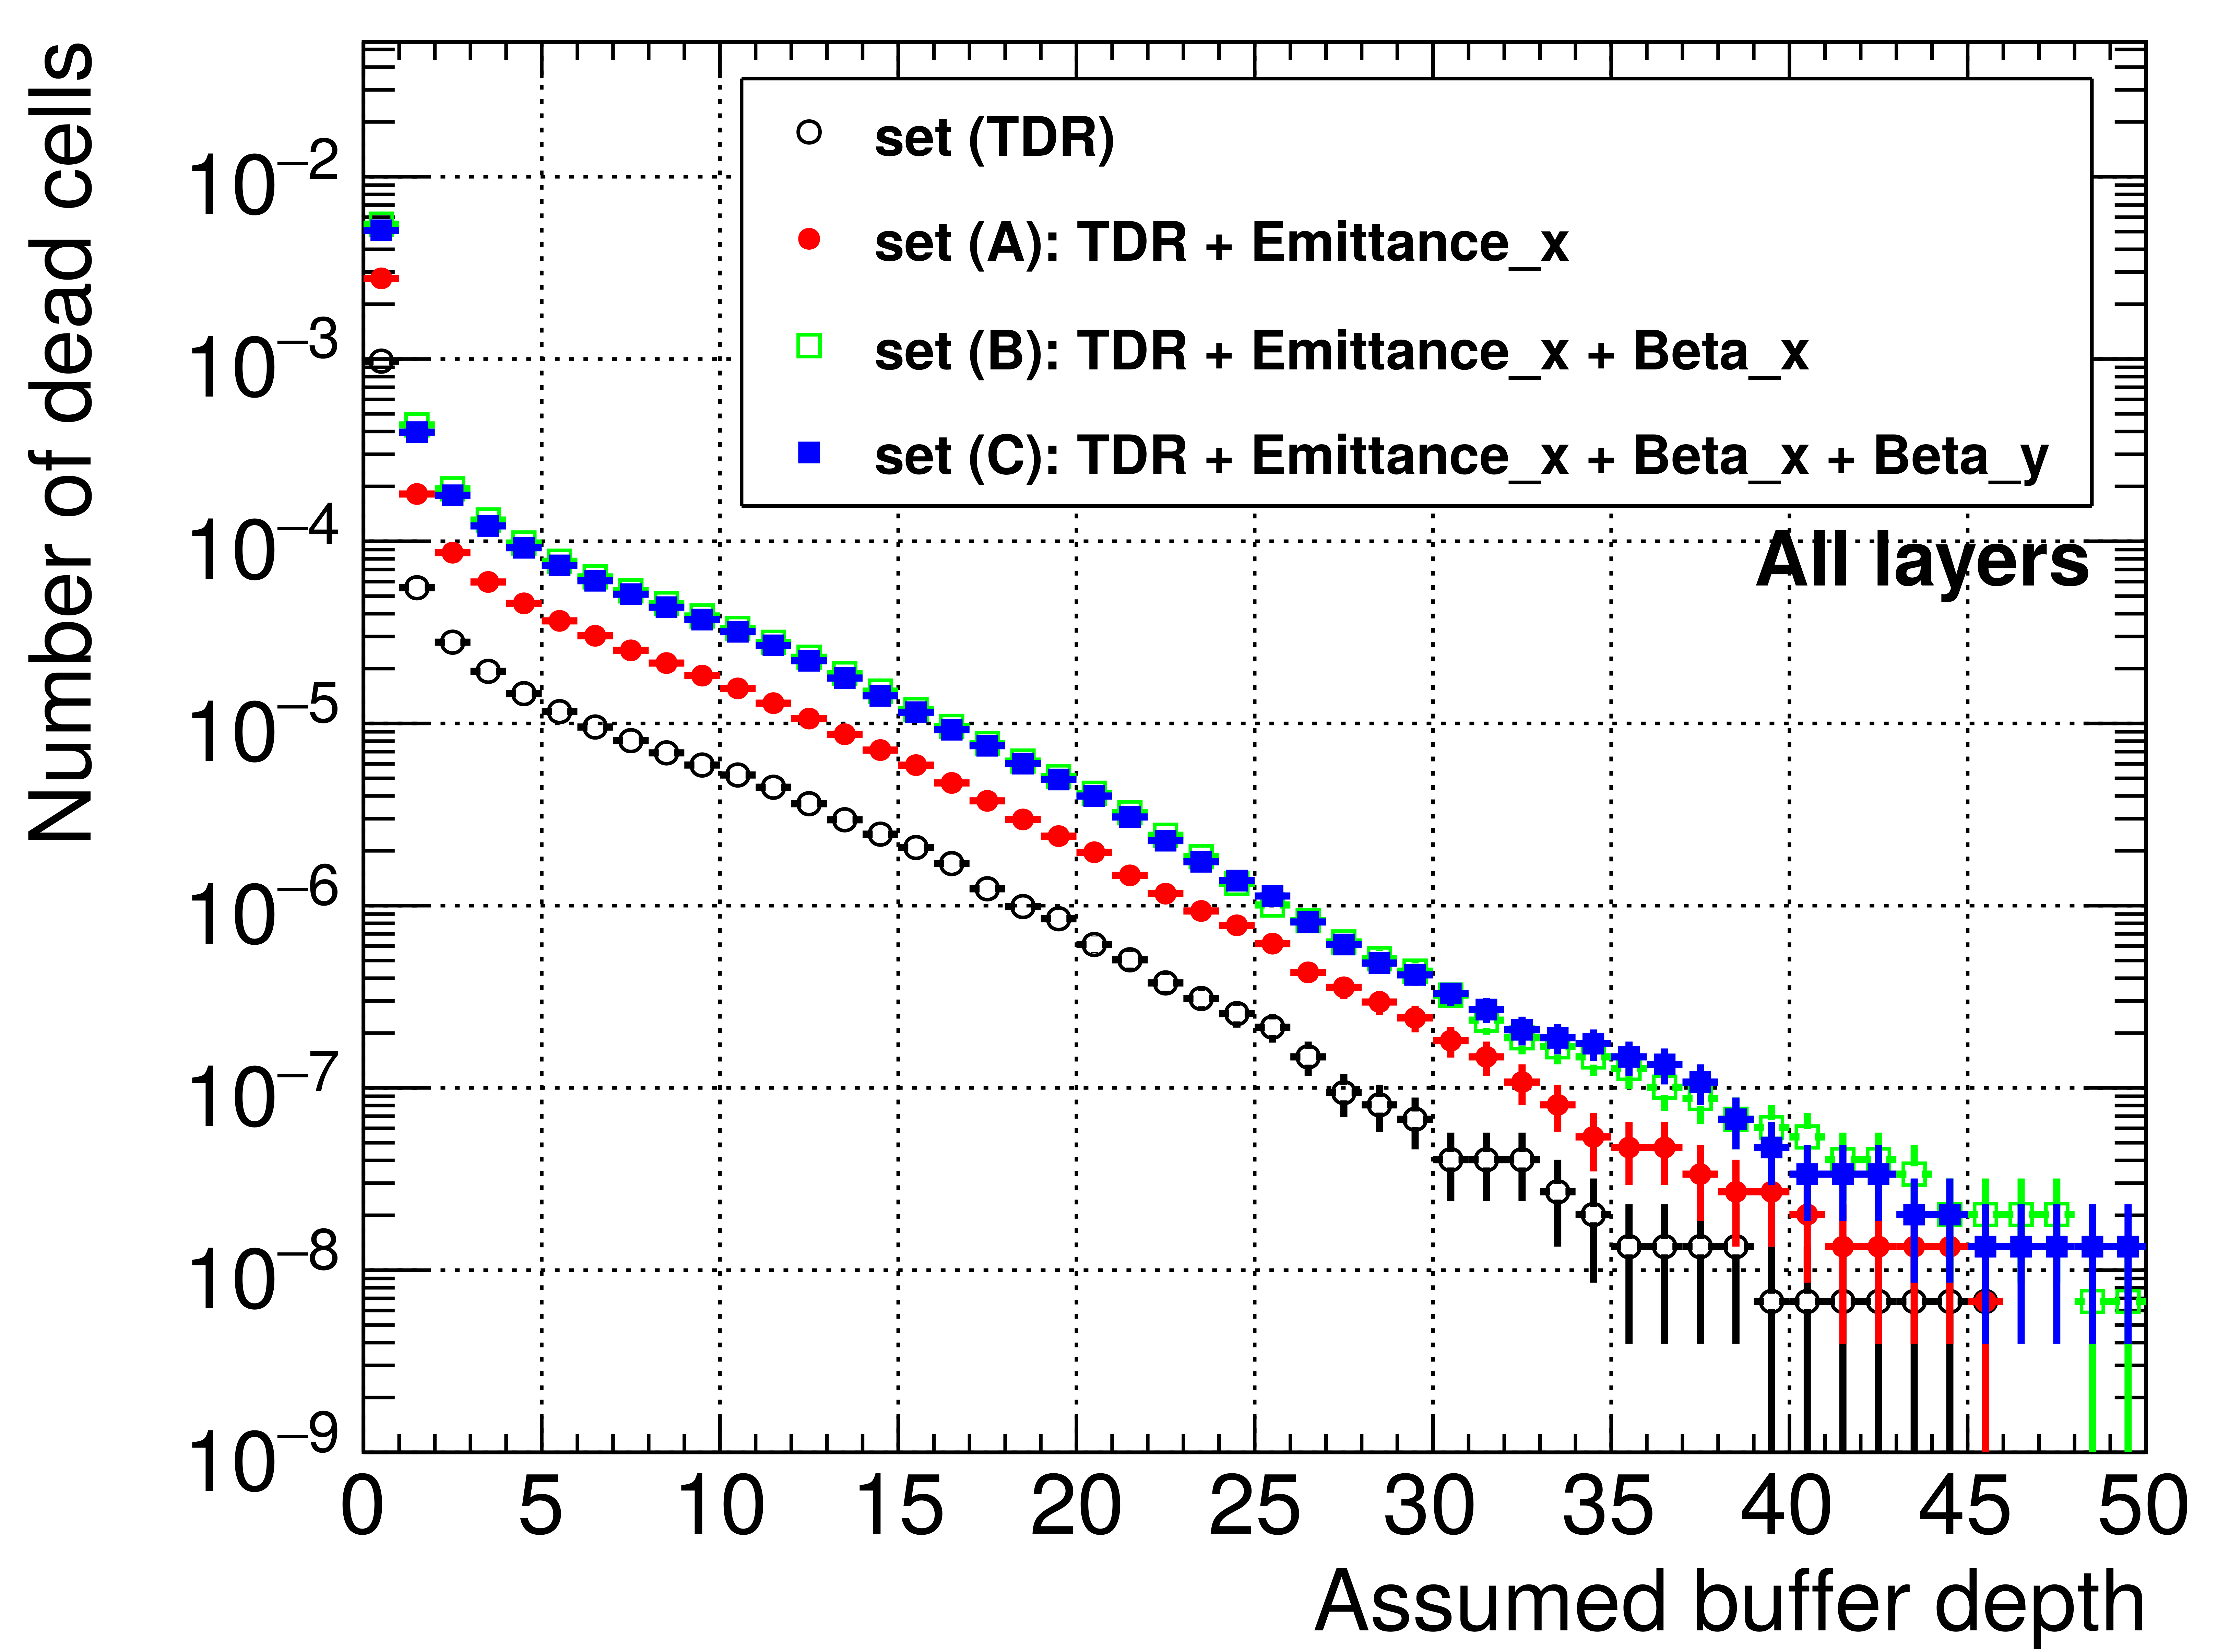
\includegraphics[width=\textwidth]{Figures/Pairs/Occupancy_Comparison_All_layers_deadcells_ILC250_ALL_SETS_5T_w_antiDiD_SiVertexEndcap.png}
   \caption{Vertex detector \textbf{endcaps}, ratio of dead cells}
   \end{subfigure}
   \caption[Pair background occupancy in the \sid vertex detector for the ILC250]{ILC250 pair background occupancy in the \textbf{\sid vertex detector for all layers} combined, after a full bunch train (\num{1312} bunch crossings).
   Figure (a) shows the occupancy in the vertex detector barrel, normalized by the total number of cells of all vertex detector barrel layers.
   Figure (b) shows the ratio of the dead cells in the vertex detector barrel with respect to the total number of cells.
   Figures (c) and (d) show the equivalent plots for the vertex detector endcaps.
   In all figures, the four different beam parameter sets for the ILC250 are compared.
   }
   \label{fig:PairBkg:ILC250_Occupancy}
 \end{figure}

  \begin{figure}
 \centering
  \begin{subfigure}[b]{0.49\textwidth}
   \centering
    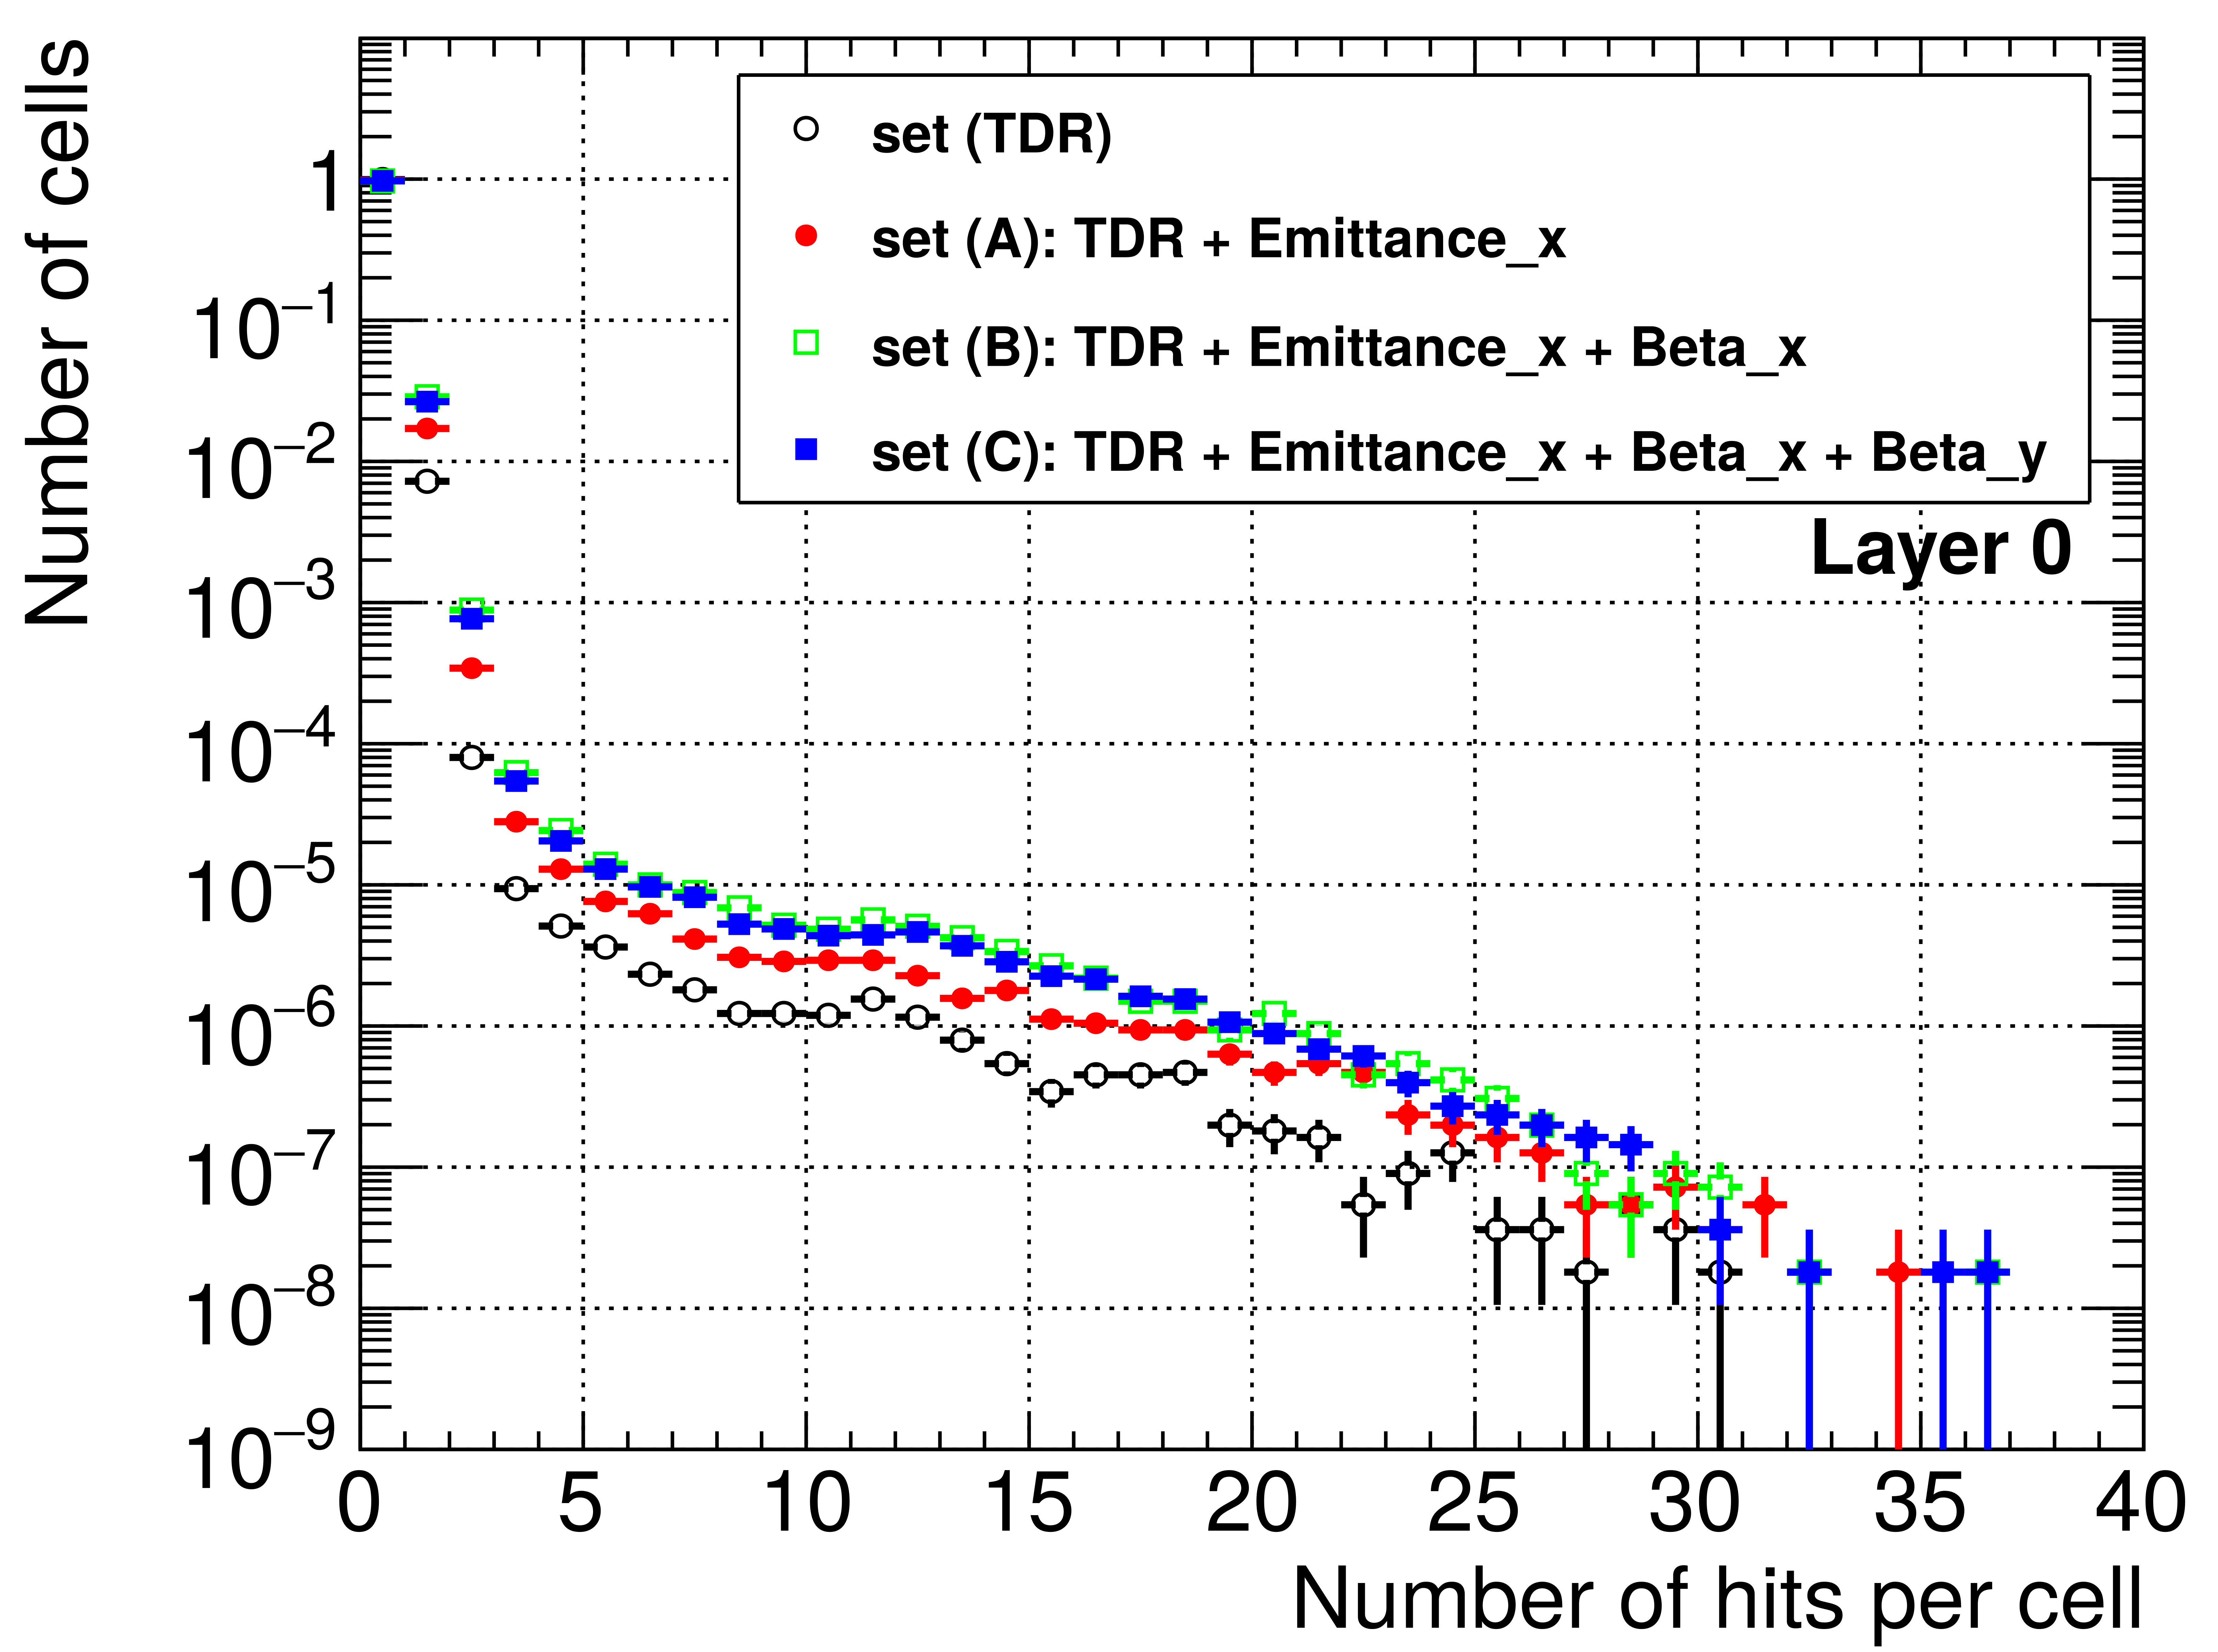
\includegraphics[width=\textwidth]{Figures/Pairs/Occupancy_Comparison_Layer_0_numcells_ILC250_Comparison_ALL_SETS_5T_w_antiDiD_LEG.png}
   \caption{Vertex detector \textbf{barrel}, normalized occupancy}
   \end{subfigure}
   \hfill
    \begin{subfigure}[b]{0.49\textwidth}
   \centering
    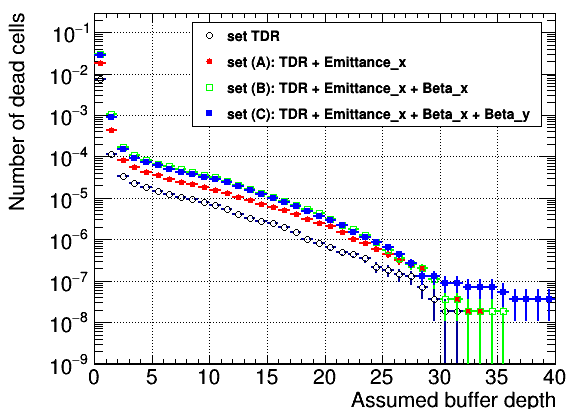
\includegraphics[width=\textwidth]{Figures/Pairs/Occupancy_Comparison_Layer_0_deadcells_ILC250_Comparison_ALL_SETS_5T_w_antiDiD_LEG.png}
   \caption{Vertex detector \textbf{barrel}, ratio of dead cells}
   \end{subfigure}\\
  \begin{subfigure}[b]{0.49\textwidth}
   \centering
    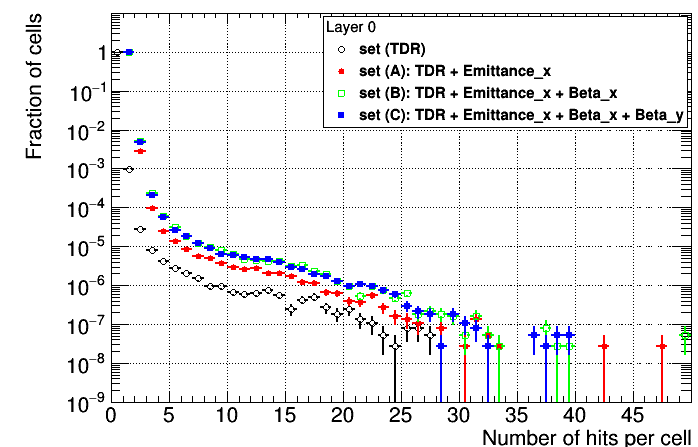
\includegraphics[width=\textwidth]{Figures/Pairs/Occupancy_Comparison_Layer_0_numcells_ILC250_ALL_SETS_5T_w_antiDiD_SiVertexEndcap.png}
   \caption{Vertex detector \textbf{endcaps}, normalized occupancy}
   \end{subfigure}
   \hfill
    \begin{subfigure}[b]{0.49\textwidth}
   \centering
    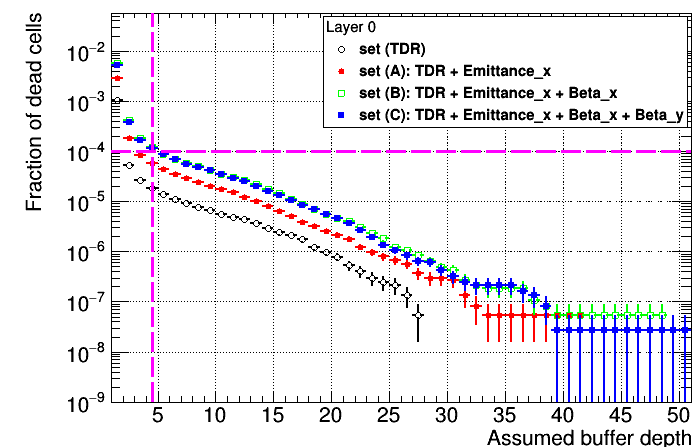
\includegraphics[width=\textwidth]{Figures/Pairs/Occupancy_Comparison_Layer_0_deadcells_ILC250_ALL_SETS_5T_w_antiDiD_SiVertexEndcap.png}
   \caption{Vertex detector \textbf{endcaps}, ratio of dead cells}
   \end{subfigure}
   \caption[Pair background occupancy in the \sid vertex detector layer 0 for the ILC250]{ILC250 pair background occupancy in the \textbf{innermost \sid vertex detector layer}, after a full bunch train (\num{1312} bunch crossings).
   Figure (a) shows the occupancy in the innermost vertex detector barrel layer, normalized by the total number of cells of this layer.
   Figure (b) shows the ratio of the dead cells in the innermost vertex detector barrel layer with respect to the total number of cells of this layer.
   Figures (c) and (d) show the equivalent plots for the vertex detector endcaps.
   In all figures, the four different beam parameter sets for the ILC250 are compared.
   }
   \label{fig:PairBkg:ILC250_Occupancy_Layer0}
 \end{figure}
However, combining the hits of all five vertex detector layers does not provide a meaningful picture of the occupancy in the individual layers.
Figure~\ref{fig:PairBkg:ILC250_Occupancy_Layer0} therefore shows the normalized occupancy and the ratio of dead cells for the innermost vertex detector layer only, again for the barrel and the endcaps separately.
Additionally, the results for all individual layers are presented in  Figures~\ref{fig:PairBkg:ILC250_Occupancy_Layers_VXDBarrel} and~\ref{fig:PairBkg:ILC250_Occupancy_Layers_VXDEndcap} in the Appendix, as well as in Table~\ref{tab:ILC250_results}.
\\For the barrel, the innermost layer is expected to suffer from a larger pair background occupancy than the other layers.
In Figure~\ref{fig:PairBkg:ILC250_Occupancy_Layer0} (a), the normalized occupancy in all sets is indeed larger by almost one order of magnitude compared to Figure~\ref{fig:PairBkg:ILC250_Occupancy} (a).
The number of dead cells for a buffer depth of four, shown in Figure~\ref{fig:PairBkg:ILC250_Occupancy_Layer0} (b), is now close to the critical limit of \num{e-4} of all cells.
For set (A), the ratio of dead cells for this buffer depth is about \num{4e-5}.
For sets (B) and (C), the ratio reaches about \num{8e-5} of all cells in this innermost layer.
\\For the endcaps, the plots for the innermost layer only do not show a significant difference to the plots for all layers combined.
In contrast to the vertex barrel layers, the endcap layers are perpendicular to the incoming pair background particles, and are hit in approximately equal amounts.
Plotting the combined occupancy for all endcap layers is in this case therefore a realistic representation of the individual layers.
 %------------------
\newcolumntype{L}[1]{>{\raggedright\let\newline\\\arraybackslash\hspace{0pt}}m{#1}}
\newcolumntype{C}[1]{>{\centering\let\newline\\\arraybackslash\hspace{0pt}}m{#1}}
\newcolumntype{G}[1]{>{\columncolor{Gray}\centering\let\newline\\\arraybackslash\hspace{0pt}}m{#1}}
\newcolumntype{R}[1]{>{\raggedleft\let\newline\\\arraybackslash\hspace{0pt}}m{#1}}
%\newcolumntype{G}[1]{>{\columncolor{Gray}\raggedleft\let\newline\\\arraybackslash\hspace{0pt}}m{#1}}
%-----------------
 \begin{table}
\caption[Results of the ILC250 pair background occupancy study]{Results of the pair background occupancy study for the different beam parameter sets of the ILC stage at \SI{250}{\GeV} center-of-mass energy.
For a buffer depth of four, the ratios of dead cells caused by the pair background occupancy are listed for the individual layers of the vertex detector barrel and endcaps.}
\label{tab:ILC250_results}
\centering
\begin{tabularx}{0.77\textwidth}{c|c|C{2.2cm}G{2.2cm}C{2.2cm}C{2.2cm}}
\hline\hline
& Layer & Baseline set (TDR) & Set (A) & Set (B) & Set (C)\\
\hline
& 0 & \num{1.819e-05} &\num{4.260e-05} &\num{8.122e-05} &\num{7.326e-05}  \\
& 1 & \num{3.586e-06} &\num{1.124e-05} &\num{2.195e-05} &\num{2.042e-05}  \\
& 2 & \num{1.453e-06} &\num{5.361e-06} &\num{1.182e-05} &\num{1.032e-05}  \\
& 3 & \num{8.789e-07} &\num{2.274e-06} &\num{5.068e-06} &\num{5.131e-06} \\
\multirow{-5}{*}{\rotatebox[origin=c]{90}{\parbox[c]{1.9cm}{\cellcolor{white}\centering \sid vertex barrel}}} & 4 & \num{5.853e-07} &\num{1.756e-06} &\num{4.286e-06} &\num{3.709e-06} \\
\hline
& 0 & \num{1.378e-05} &\num{4.295e-05} &\num{8.885e-05} &\num{8.637e-05} \\
& 1 & \num{1.442e-05} &\num{4.704e-05} &\num{9.601e-05} &\num{8.943e-05} \\
& 2 & \num{1.398e-05} &\num{4.508e-05} &\num{1.059e-04} &\num{9.218e-05} \\
\multirow{-4}{*}{\rotatebox[origin=c]{90}{\parbox[c]{1.9cm}{\cellcolor{white}\centering \sid vertex endcap}}} & 3 & \num{1.616e-05} &\num{4.746e-05} &\num{1.005e-04} &\num{1.006e-04} \\
\hline\hline
\end{tabularx}
\end{table}

Overall, the increase in the beam-beam interaction does lead to a rise in the \sid vertex detector occupancy.
However, even in the innermost vertex detector layer, the occupancy for all proposed beam parameter sets for the ILC250 stage is below the critical acceptance limit of \num{e-4} for every feasible buffer depth of the detector sensor design.
The presented results of the \sid occupancy studies for the different beam parameter sets of the ILC250 stage were factored into the ILC Change Request (CR) process for CR-0016.
The Technical Change and Management Board in the end decided on set (A) for the new official ILC beam parameter set for a center-of-mass energy of \SI{250}{\GeV}, and hence approved the CR-0016~\cite{LCWS17_TCMBmeeting,CR-0016}.
The results of further studies regarding the ILC250 stage are henceforth produced with this new official beam parameter set (A).

\subsection{Dependency of the pair background occupancy on detector design choices}
Figure~\ref{fig:PairBkg:ILC250_Occupancy_SetA} shows the result from another ILC250 occupancy study, using the ILC250 parameter scheme (A).
After having studied the impact of the beam parameters, the effect of different \sid variants on the vertex detector occupancy was also examined.
The four geometry variants, which are compared in this plot, are combinations of the old or new L* value, with and without the \sid anti-DiD field.
For more information about these detector variants, please refer to Section~\ref{ILC:SiD}.
The variations on the \sid geometry do not have a significant impact on the vertex barrel occupancy. \todo{Add also for endcaps}
Nevertheless, the \sid design including the old L* value and the anti-DiD field leads to the lowest occupancy.
The occupancy of the current design (with the new L* value and the anti-DiD field) is only marginally higher.
Since the geometry of the vertex detector and all other subdetectors is unaltered in the studied \sid variants, the difference in the pair background occupancy must be caused by the impact of the L* and the anti-DiD field themselves.
The change in the L* value implies a change in the position of the BeamCal subdetector.
The anti-DiD field is designed to guide the pair background particles through the outgoing beam pipe, so that the number of pair background hits in the BeamCal is reduced.
The differences in Figure~\ref{fig:PairBkg:ILC250_Occupancy_SetA} are an indication that the \sid BeamCal affects the vertex detector occupancy from pair background particles.
For the clarification of the impact on the pair background occupancy, the following section looks at the hit distribution in the \sid detector.
 \begin{figure}
 \centering
   \begin{subfigure}[b]{0.49\textwidth}
   \centering
    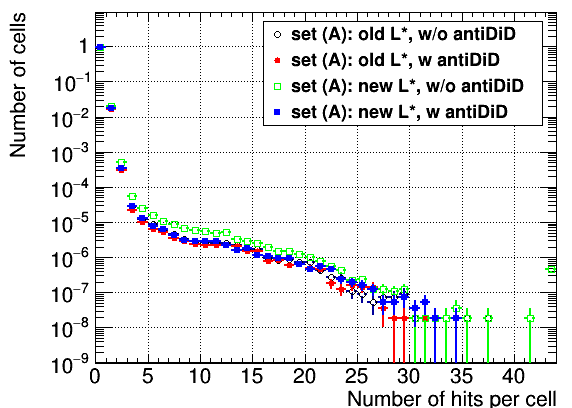
\includegraphics[width=0.6\textwidth]{Figures/Pairs/Occupancy_Comparison_Layer_0_numcells_ILC250_Comparison_Set_A_All_SiD_designs_LEG.png}
       \caption{\sid vertex \textbf{barrel}}
   \end{subfigure}
   \hfill
    \begin{subfigure}[b]{0.49\textwidth}
   \centering
    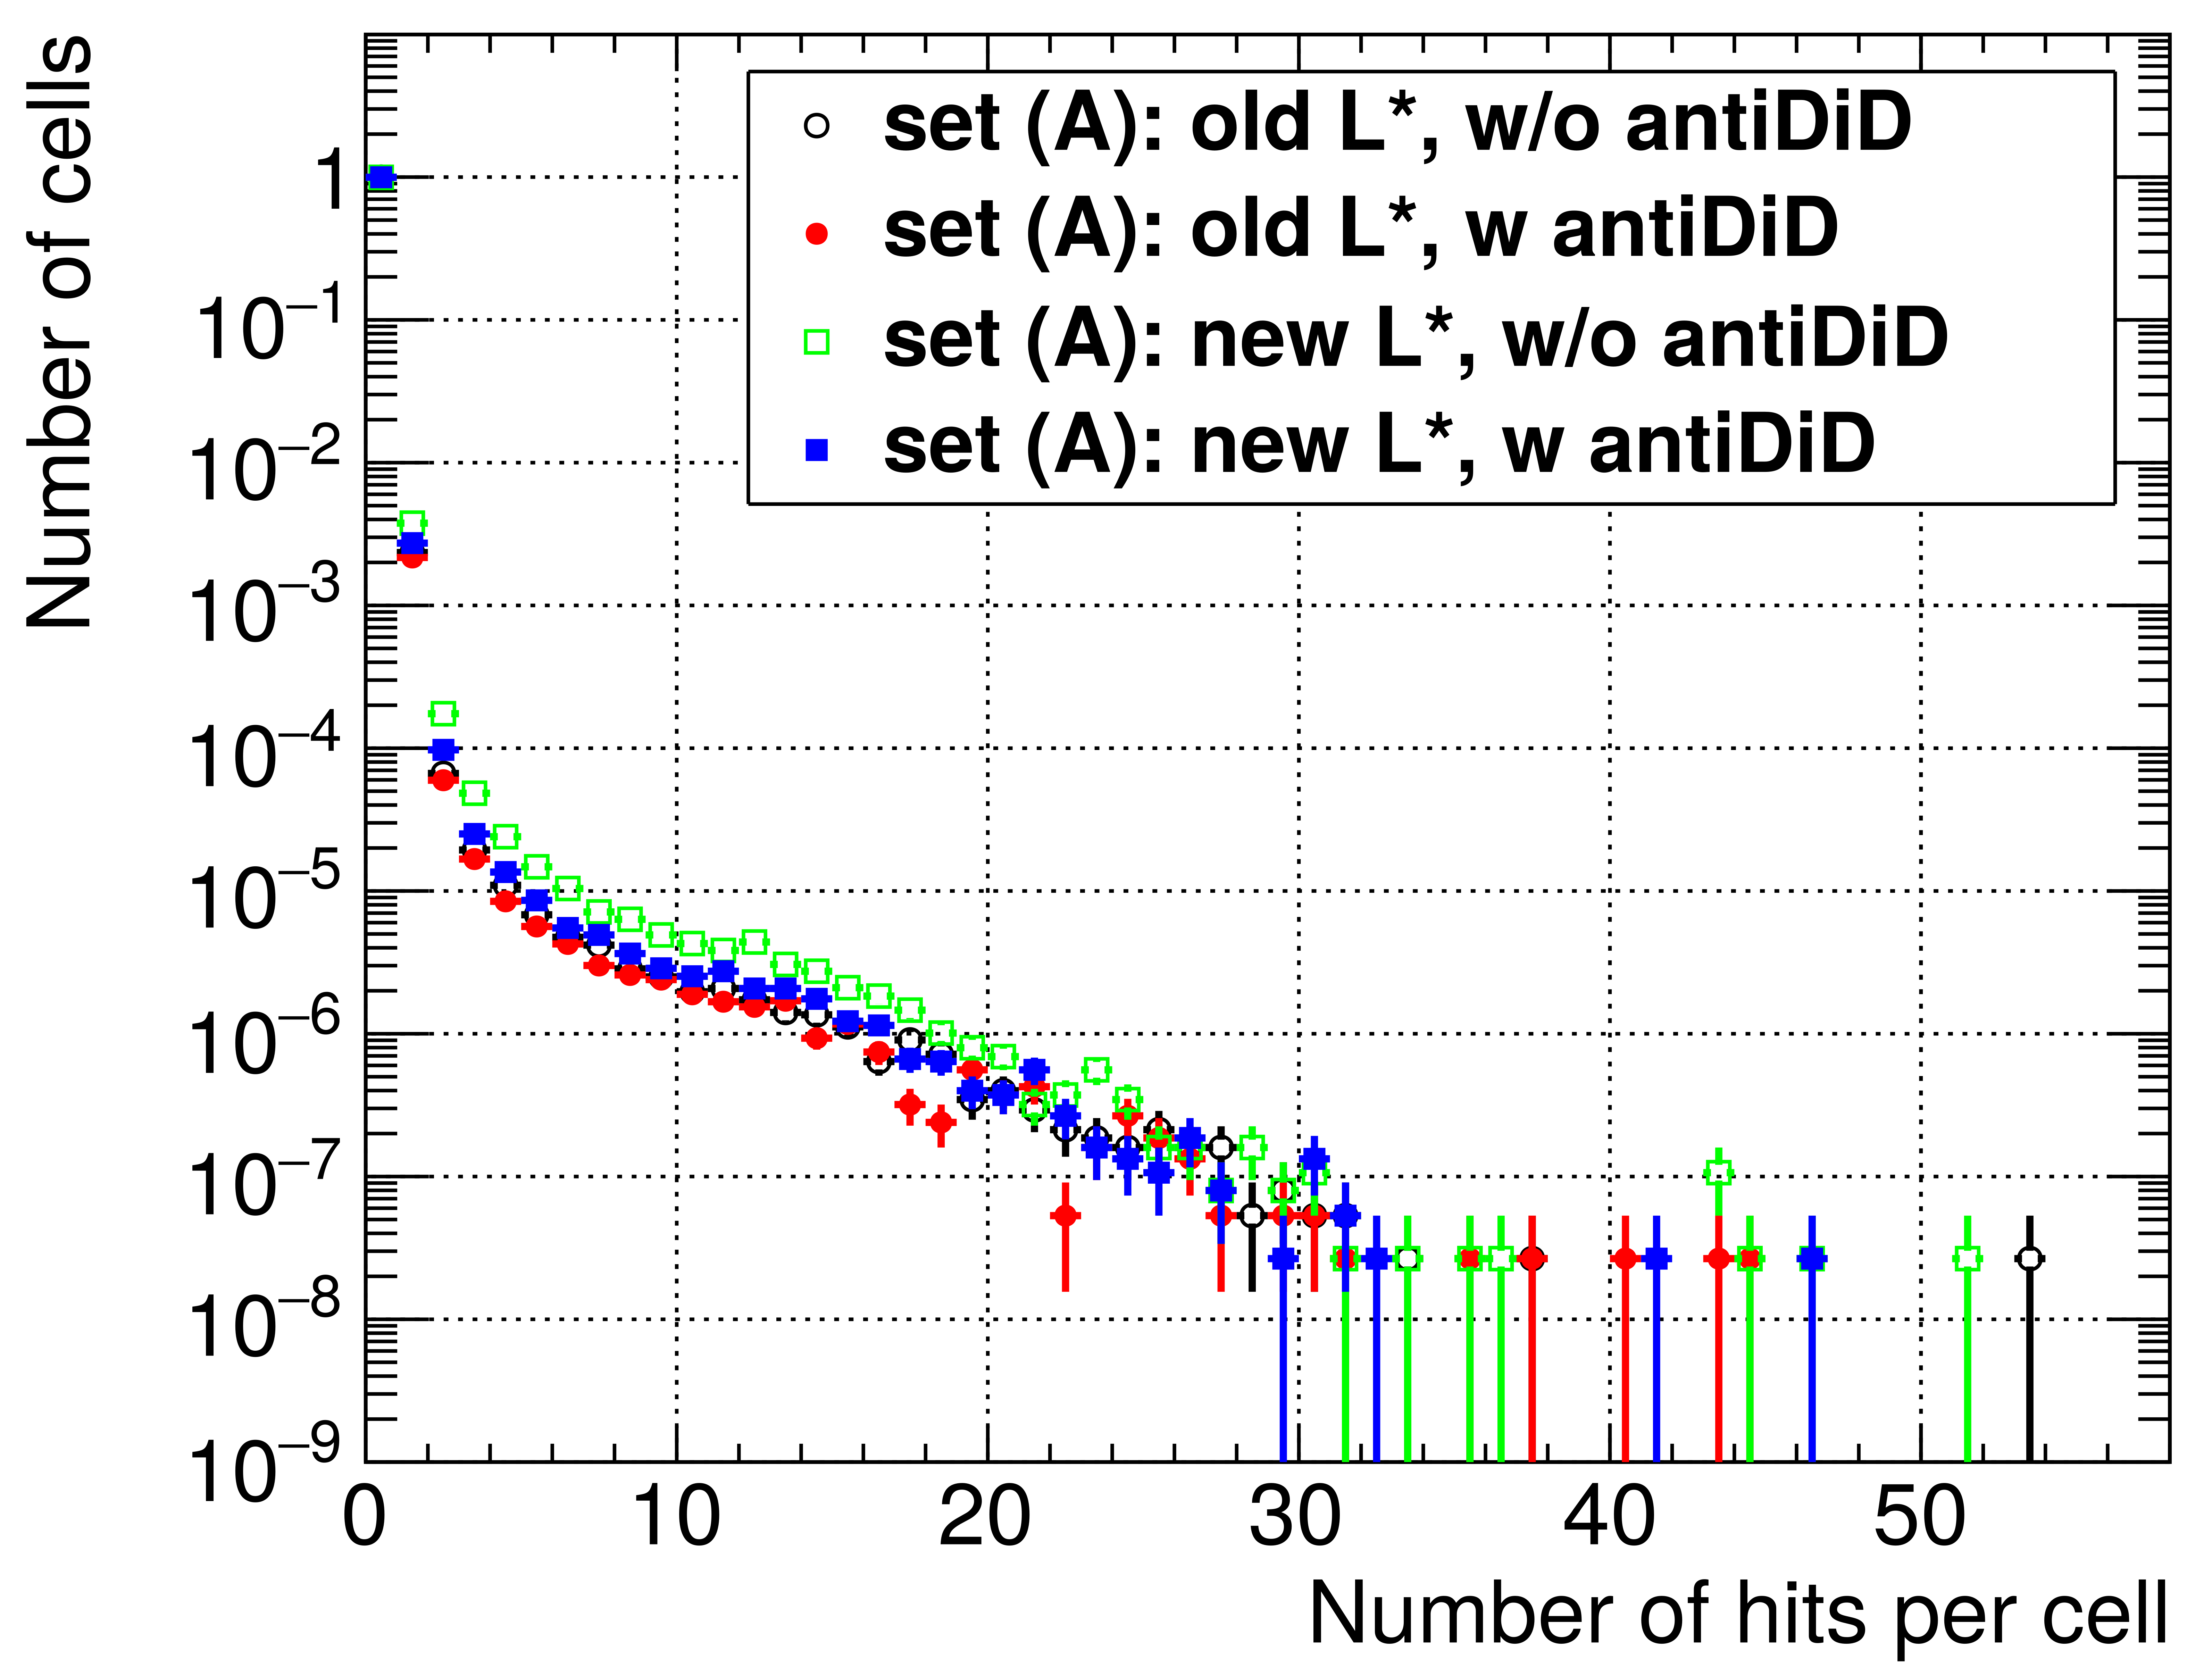
\includegraphics[width=0.6\textwidth]{Figures/Pairs/Occupancy_Comparison_Layer_0_numcells_ILC250_Comparison_Set_A_All_SiD_designs_SiVertexEndcap.png}
       \caption{\sid vertex \textbf{endcap}}
   \end{subfigure}
   \caption[Pair background occupancy in the \sid vertex detector for the ILC250 set (A) for different \sid geometry variants]{Pair background occupancy for the ILC250 parameter set (A) in the innermost \sid vertex detector layer, after a full bunch train (\num{1312} bunch crossings).
   Figures (a) and (b) show the occupancy normalized by the total number of cells of the innermost vertex detector layer for the barrel and the endcap respectively.
   Different \sid geometry variants are compared regarding their effect on the pair background occupancy.
   }
   \label{fig:PairBkg:ILC250_Occupancy_SetA}
 \end{figure}

\section{Hit maps of the \sid subdetectors}
\label{PairBkg:hitmaps}
%TODO Show with projection of hitmaps that there are more hits on edges of VertexBarrel detector (because of helix envelopes)
%TODO TH1D* histo=Layer_1->ProjectionX("ProjectionX",1,Layer_1->GetNbinsY(),"e")
As shown in the sections above, the \positron\electron pair background arises from beam-beam interactions at the IP.
Being boosted in the beam direction, and swept into the outgoing beam pipe by the anti-DiD, the hits in the \sid detector are mainly restricted to the inner subdetectors.
However, as indicated by Figure~\ref{fig:PairBkg:ILC250_Occupancy_SetA}, the \sid geometry variants have an impact on the vertex detector occupancy from the \positron\electron pairs.
\\Figure~\ref{fig:PairBkg:Origins_Map} shows maps of the pair background vertices in the \sid detector.
A cut was applied to only show the vertices of the pairs, which will hit the vertex detector in the given time intervals: up to \SI{10}{\nano\second} (Figure~\ref{fig:PairBkg:Origins_Map} (a)), and between \SI{20}{\nano\second} and \SI{30}{\nano\second} after the bunch crossing (Figure~\ref{fig:PairBkg:Origins_Map} (b)).
In this way, it becomes clear whether the background particles originate at the IP only, or whether they also backscatter from other subdetectors.
In the first \SI{10}{\nano\second}, the majority of particles, which hit the vertex detector, comes from the IP.
Also a few backscatter particles are visible, originating from the innermost detector layers and the central subdetectors.
A few nanoseconds later however, between \SI{20}{\nano\second} and \SI{30}{\nano\second}, particles hit the vertex detector that were backscattered from the BeamCal positioned about \SI{3.2}{\meter} from the IP.
These pair background particles traveled from the IP towards the BeamCal, where they hit the material and backscattered back towards the vertex detector.
\\The distance from the IP towards the BeamCal and back, which the particles have traveled, takes of the order of several tens of nanoseconds.
This time gap is visible in Figure~\ref{fig:PairBkg:Hittime}, which shows the radial position of the hits in the vertex detector barrel and endcaps as a function of the hit time.
First, the vertex detector is hit by \positron\electron pairs arriving directly from the IP.
Before pairs have traveled towards the BeamCal and have backscattered, the vertex detector does not see any further hits.
Only from around \SI{20}{\nano\second} on, particles arrive again at the vertex detector.
\\This hit time distribution offers the possibility of reducing the background occupancy through time gates.
By applying a trigger such that those particles are dismissed, which are hitting the vertex detector between \SI{10}{\nano\second} and \SI{50}{\nano\second} after the bunch crossing for example, the number of pair background hits can be reduced by about \SI{12}{\percent}~\cite[p. 27]{SiDBkgNote}.
 \begin{figure}
 \centering
  \begin{subfigure}[b]{0.49\textwidth}
   \centering
    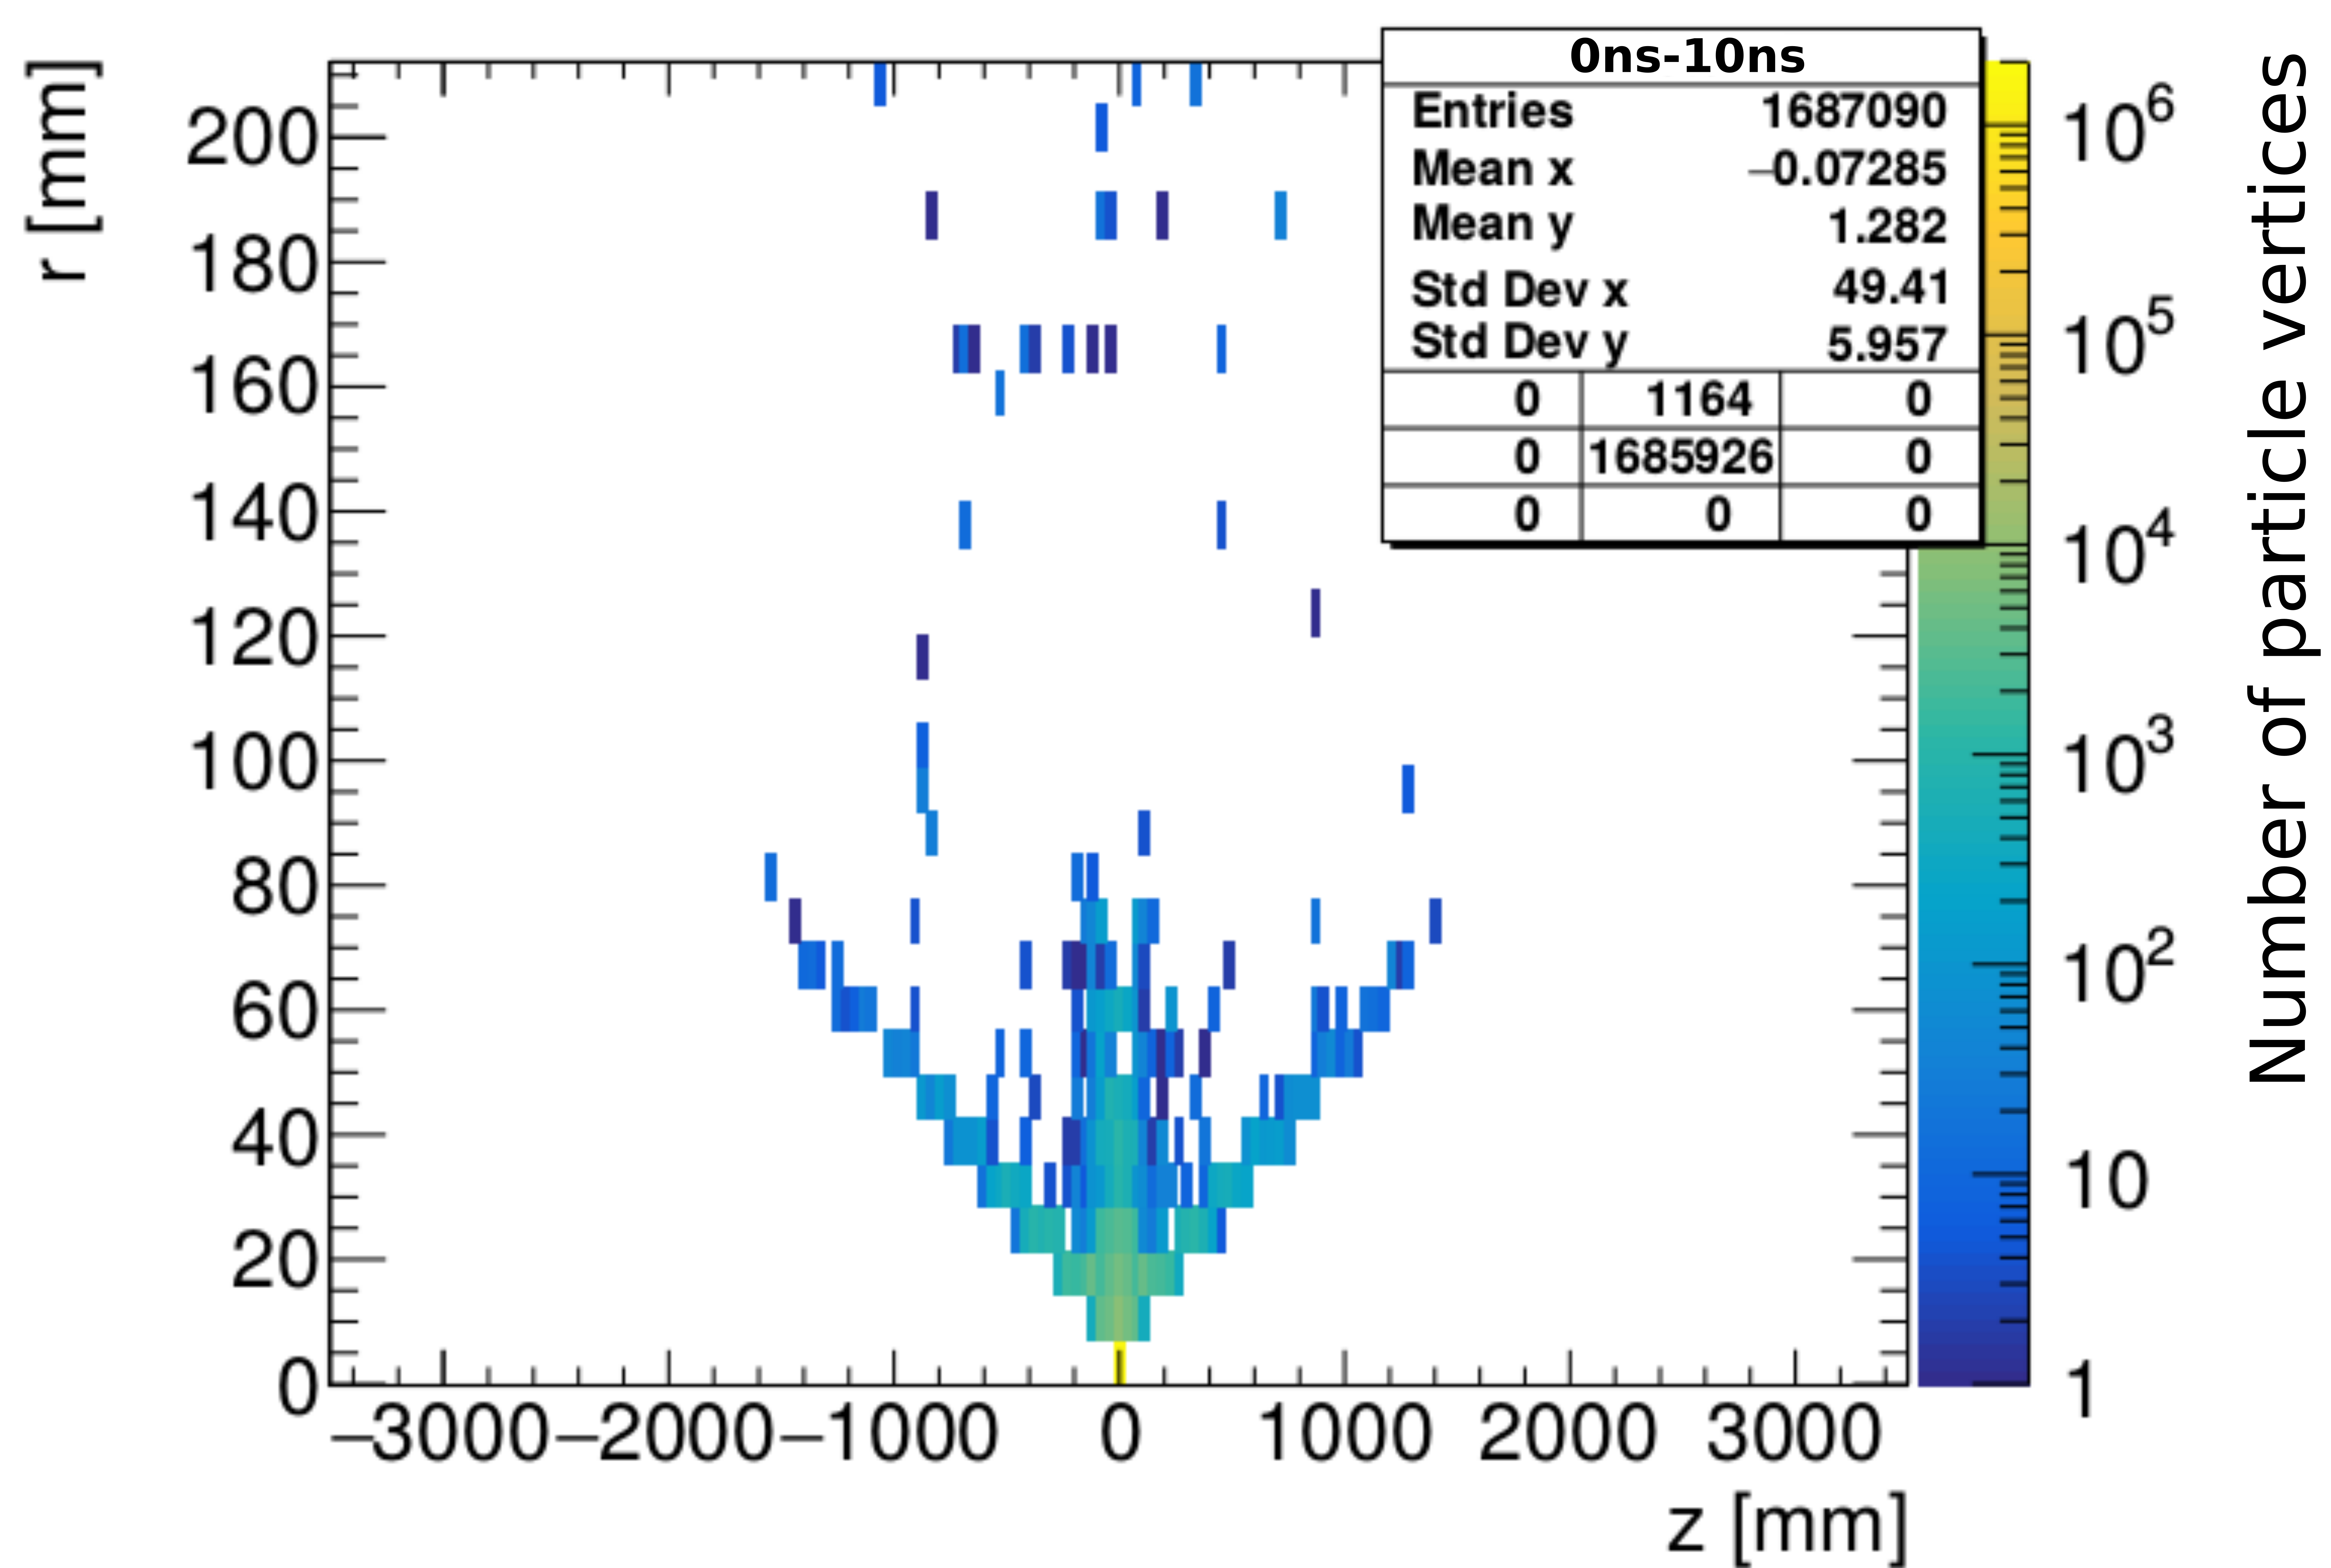
\includegraphics[width=\textwidth]{Figures/Pairs/hitmaps_particleorigins_hittime_0_10_SiVertexEndcapSiVertexBarrel_SiDNote.png}
   \caption{Hit time: \SI[detect-all]{0}{\nano\second} - \SI[detect-all]{10}{\nano\second}}
   \end{subfigure}
   \hfill
    \begin{subfigure}[b]{0.49\textwidth}
   \centering
    \includegraphics[width=\textwidth]{Figures/Pairs/hitmaps_particleorigins_hittime_20_30_SiVertexEndcapSiVertexBarrel_SiDNote.png}
   \caption{Hit time: \SI[detect-all]{20}{\nano\second} - \SI[detect-all]{30}{\nano\second}}
   \end{subfigure}
   \caption[Pair background vertex maps in the \sid detector]{Map of the pair background particle vertices in the \sid detector after one bunch crossings.
   Only those vertices are shown, which originate from pair background particles hitting the \sid vertex detector in the given time intervals.
   Figure (a) shows the vertices of those pairs, which hit the vertex detector up to \SI[detect-all]{10}{\nano\second} after the bunch crossing.
   Similarly, Figure (b) shows the vertices of pairs hitting the vertex detector between \SI[detect-all]{20}{\nano\second} and \SI[detect-all]{30}{\nano\second} after the bunch crossing.
   }
   \label{fig:PairBkg:Origins_Map}
 \end{figure}
 
  \begin{figure}[h]
 \centering
  \begin{subfigure}[b]{0.49\textwidth}
   \centering
    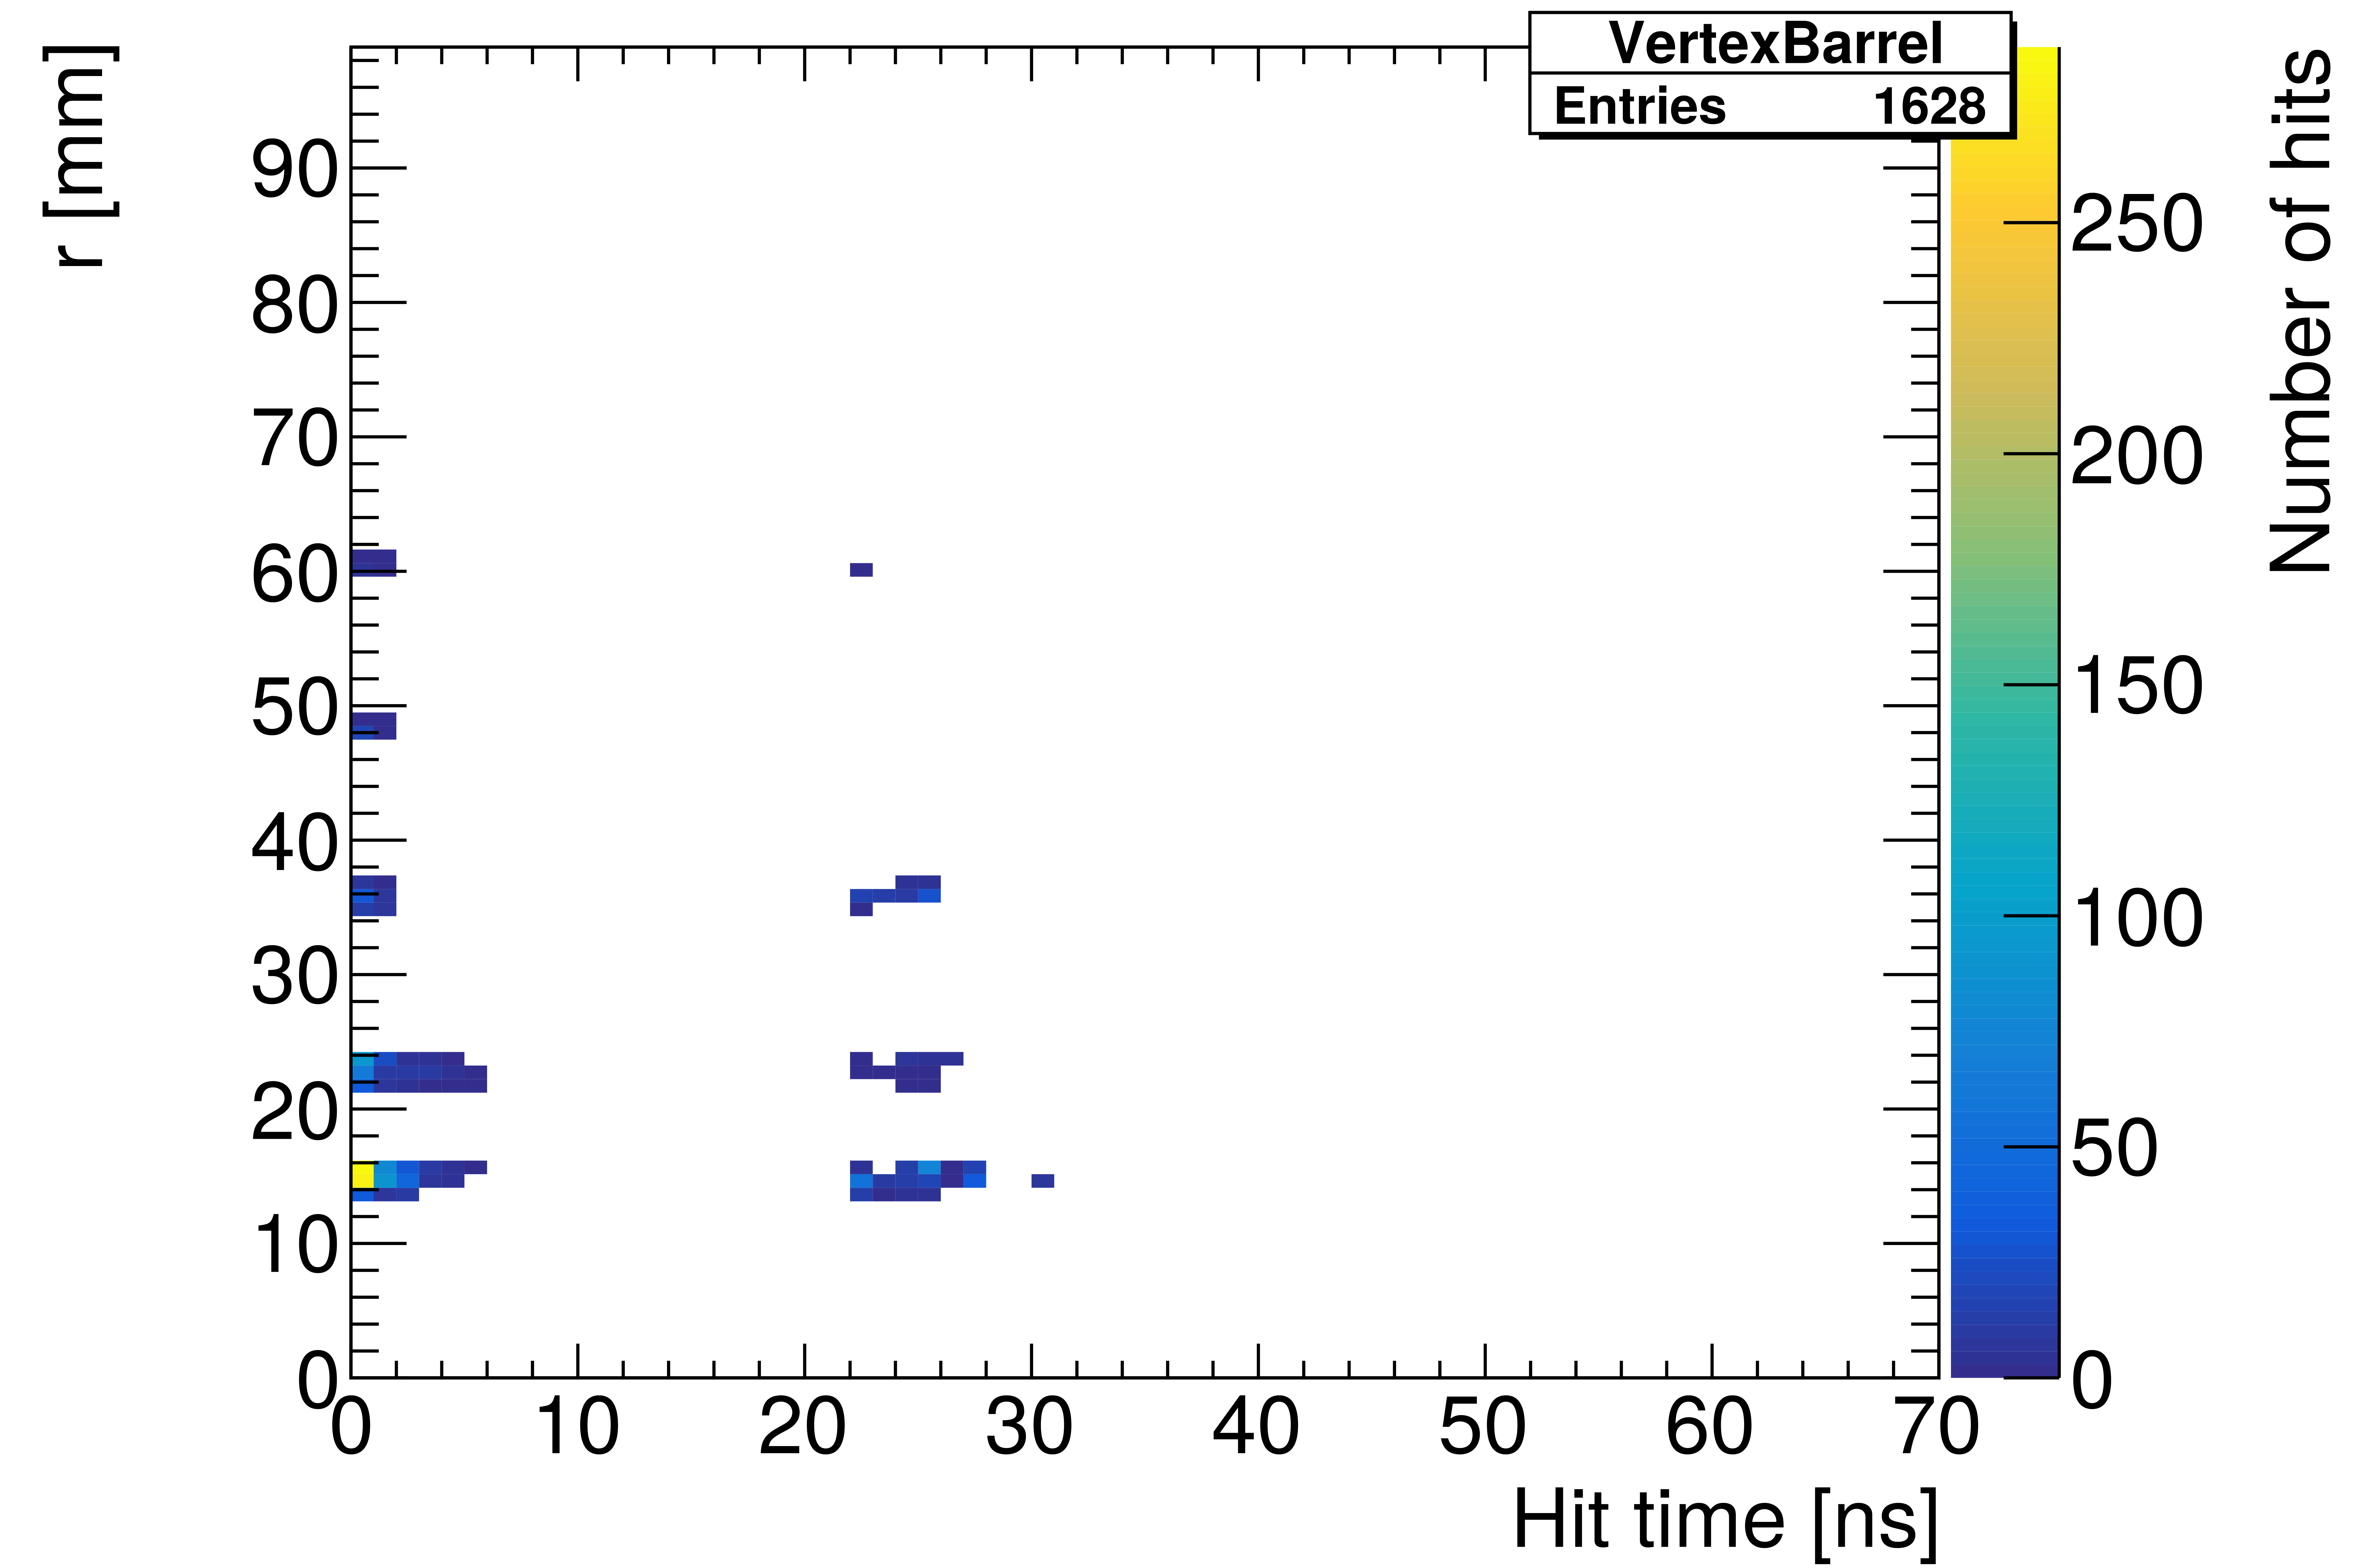
\includegraphics[width=\textwidth]{Figures/Pairs/hittime_SiVertexBarrel.png}
   \caption{Vertex detector \textbf{barrel}}
   \end{subfigure}
   \hfill
    \begin{subfigure}[b]{0.49\textwidth}
   \centering
    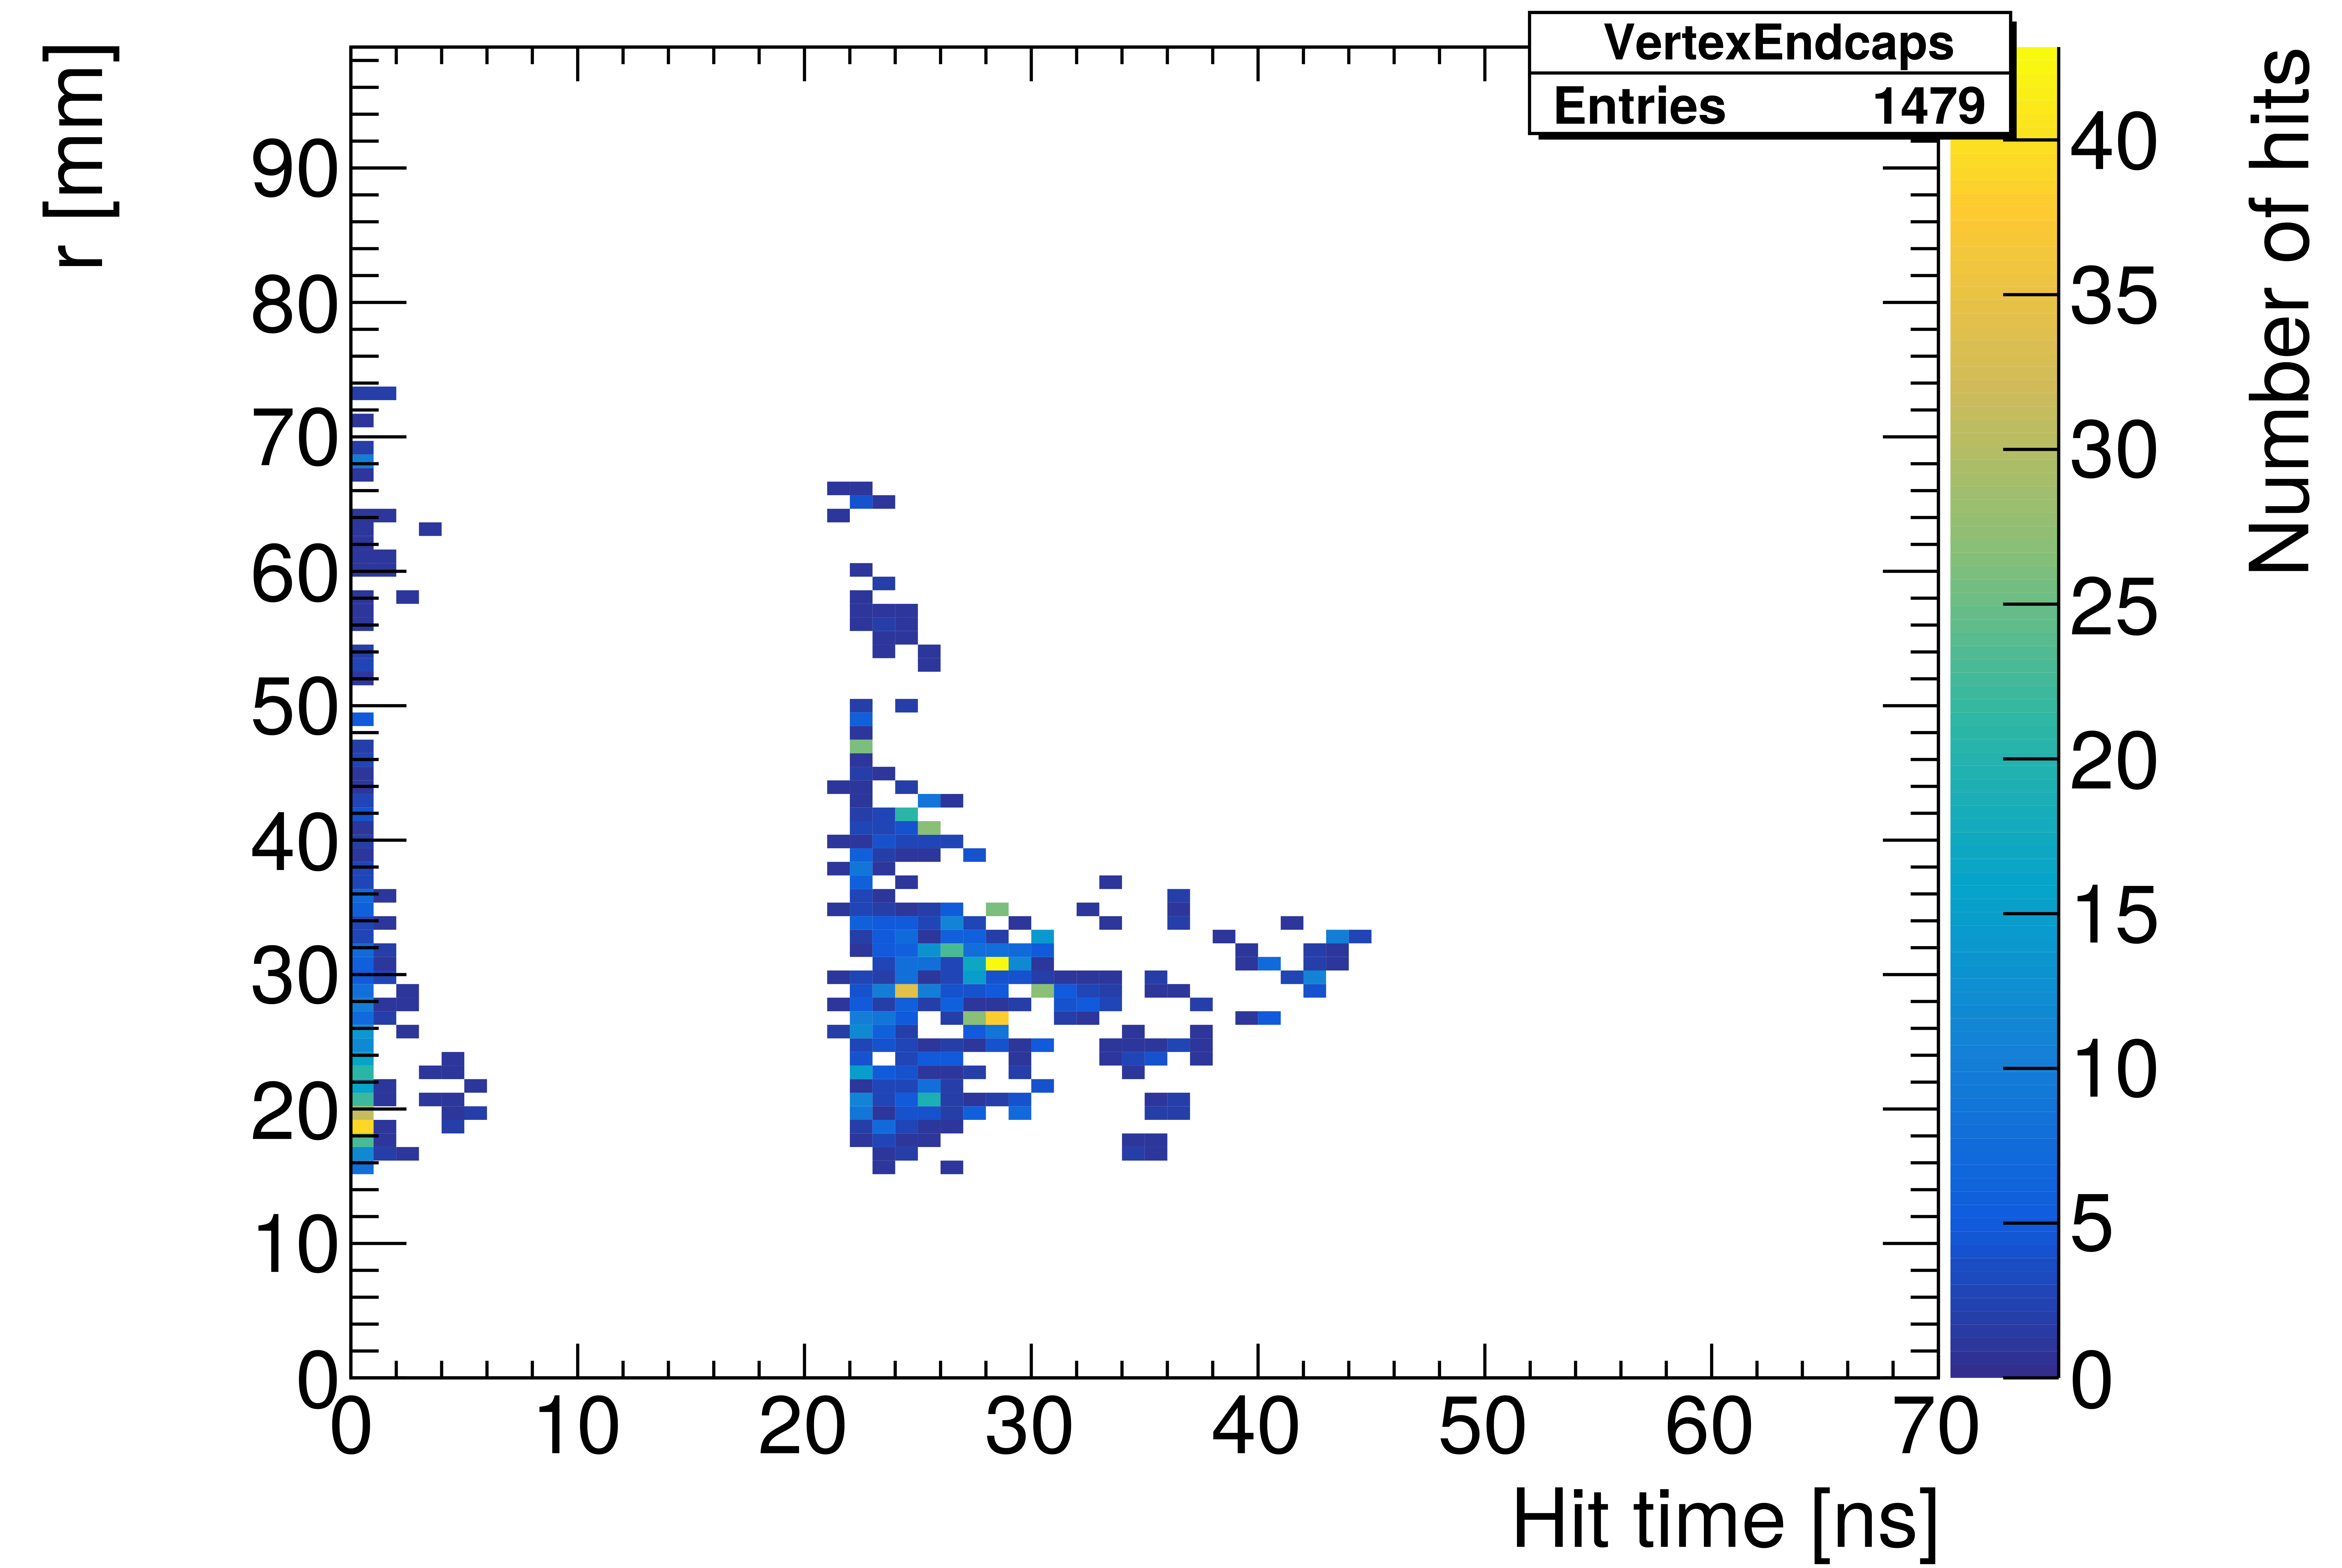
\includegraphics[width=\textwidth]{Figures/Pairs/hittime_SiVertexEndcap.png}
   \caption{Vertex detector \textbf{endcaps}}
   \end{subfigure}
   \caption[Pair background hit time maps in the \sid vertex detector]{Map of the pair background particle hits in the \sid vertex detector as a function of the hit time after one bunch crossings.
   Figures (a) and (b) show the radial position of hits in the vertex detector barrel and endcaps respectively.
   }
   \label{fig:PairBkg:Hittime}
 \end{figure}
 
 
\section{Comparing the pair background occupancy of different ILC stages}
As it has been clarified in the previous sections, the pair background envelopes and the arising vertex detector occupancy are dependent on several factors:
the ILC beam parameters, the center-of-mass energy, and the \sid geometry regarding the BeamCal and the anti-DiD field.
\\However, due to the interplay of several of these factors, the dependencies are also not obvious in certain cases, as can be seen in Figure~\ref{fig:PairBkg:ILC500-ILC250_Occupancy}.
The plots compare the \sid vertex detector occupancies from the pair background arising at a center-of-mass energy of \SI{250}{\GeV} and \SI{500}{\GeV}.
With the new ILC250 beam parameter set, the resulting occupancies at both center-of-mass energies are very similar, with the occupancy at the ILC500 being higher by a few percent.
The reduction in the beam emittance for the ILC250 stage increases the beam-beam interactions such that the differences between the center-of-mass energies (and therefore the pair background momenta distributions) are nearly compensated.
For the \sid detector, this leads to the positive implication that the vertex detector readout architecture can be designed to be suitable for both ILC stages with respect to the pair background.\\
\begin{figure}
 \centering
  \begin{subfigure}[b]{0.49\textwidth}
   \centering
    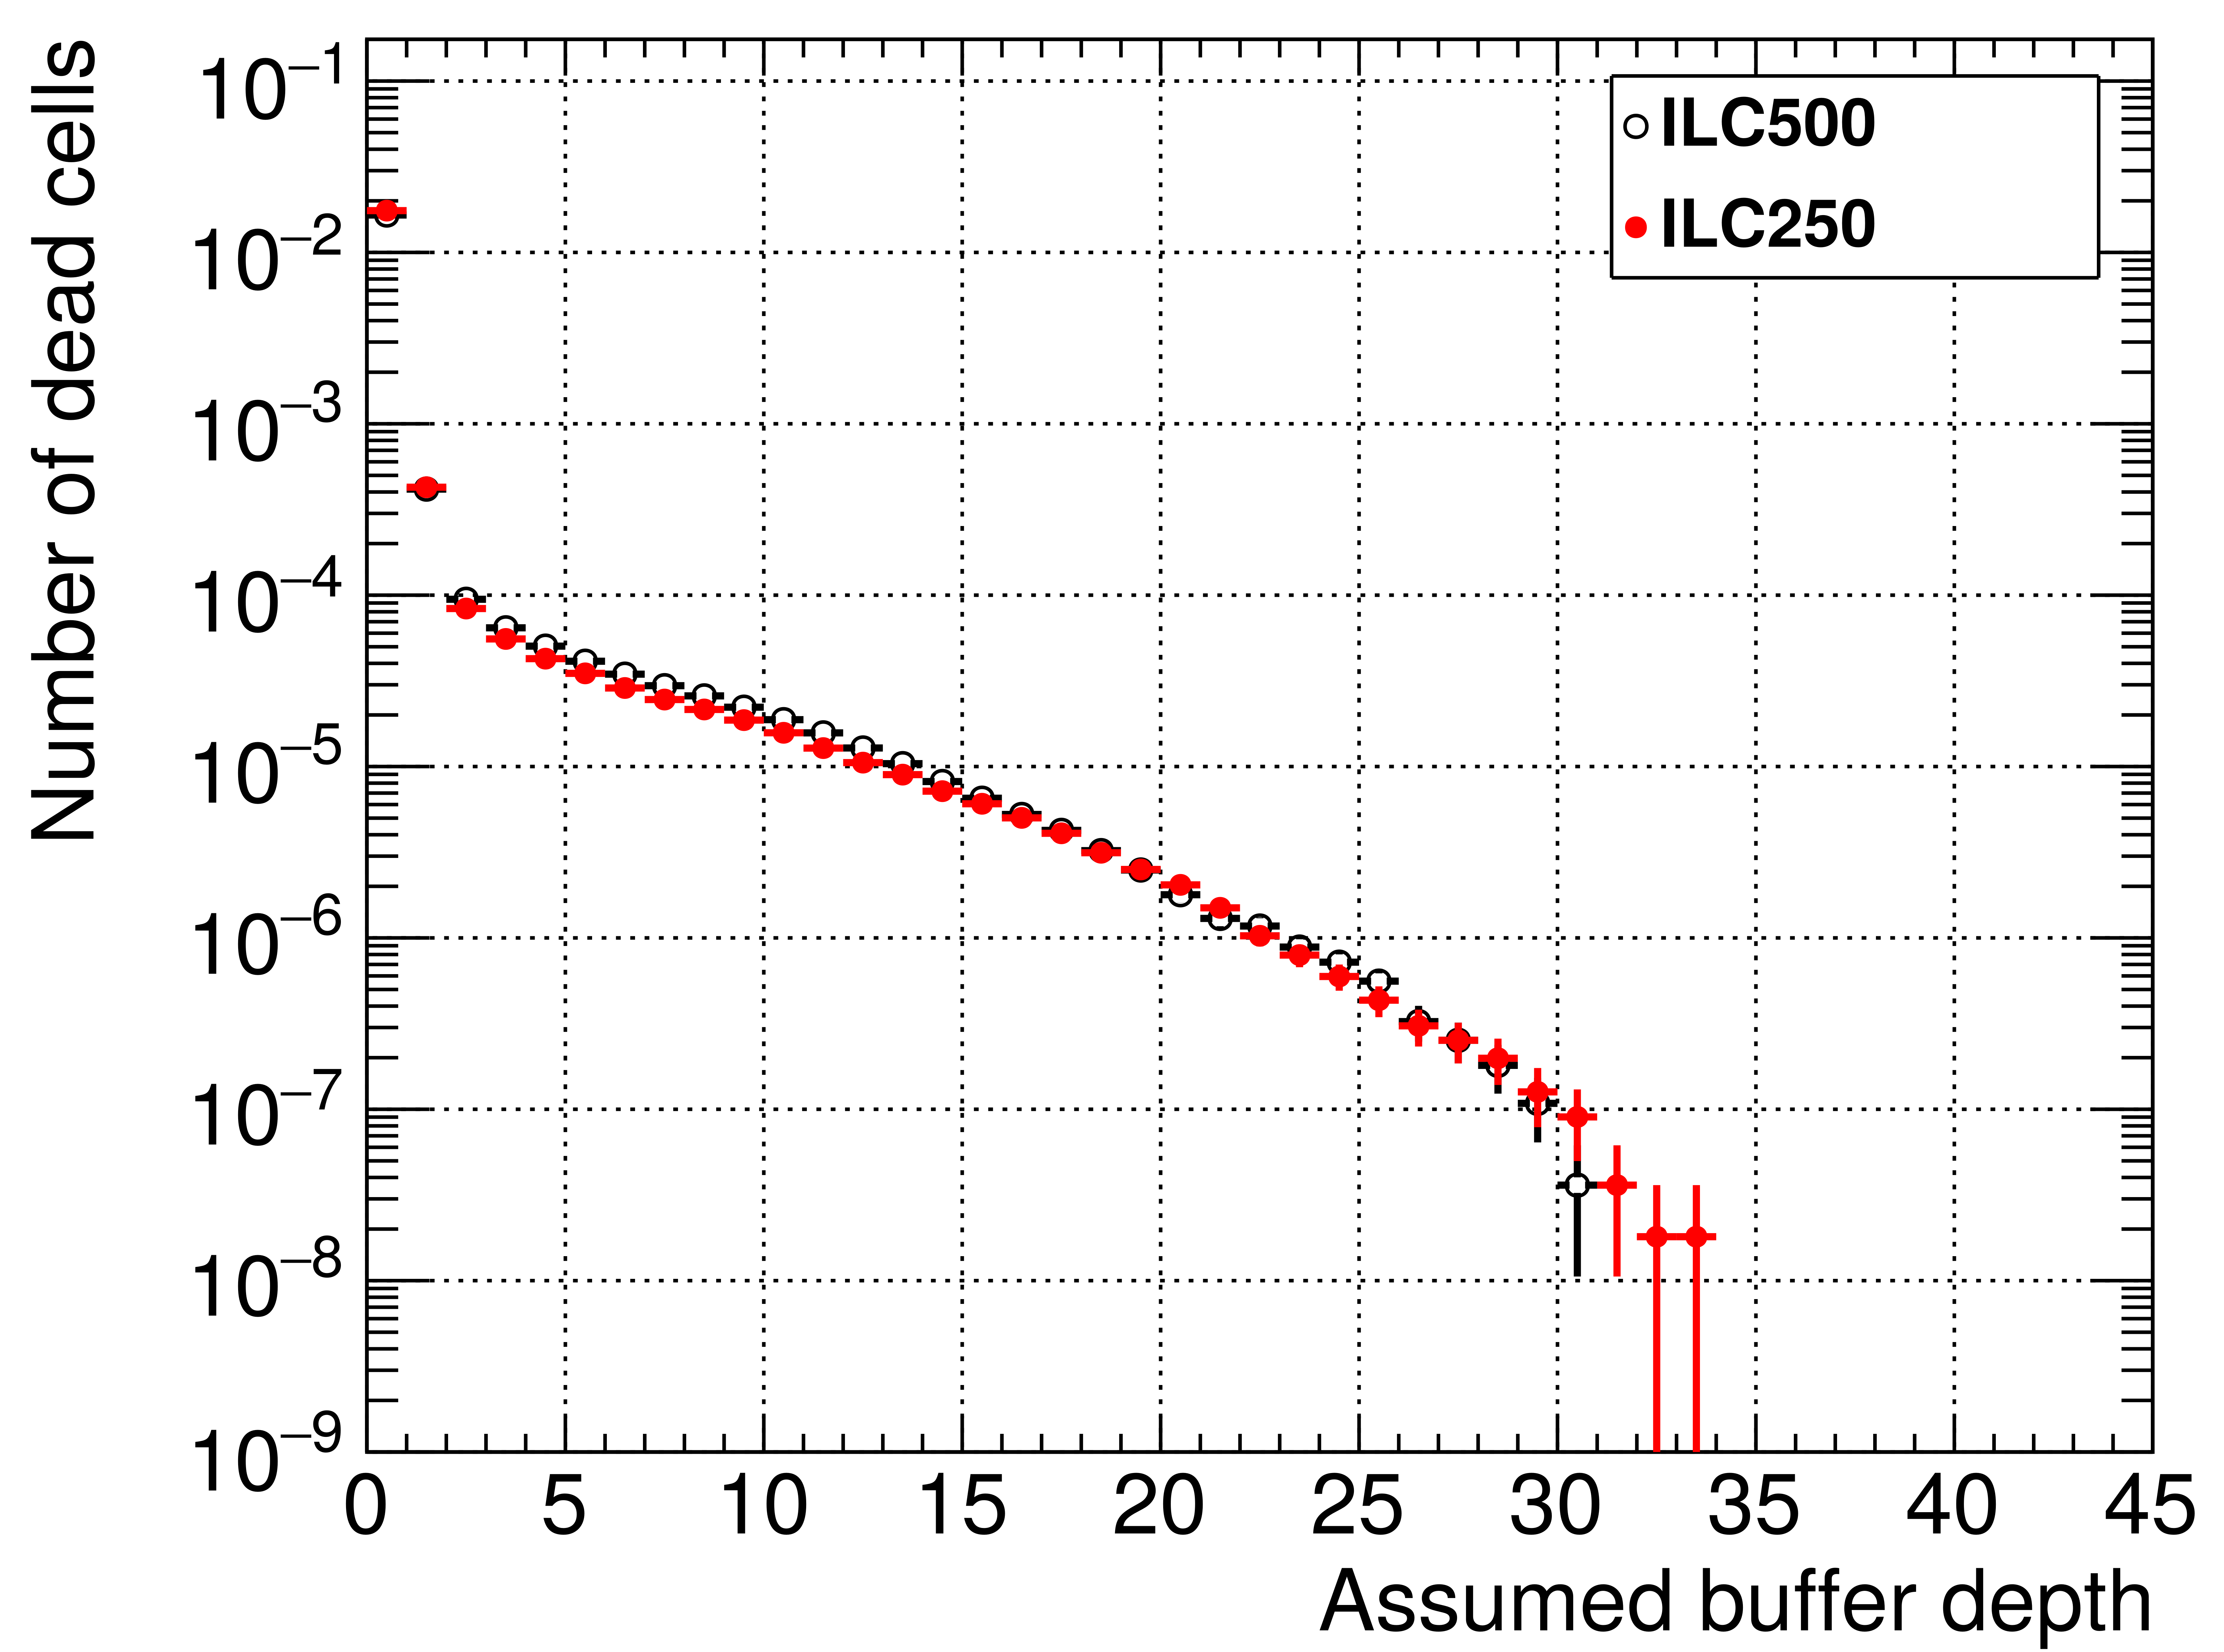
\includegraphics[width=\textwidth]{Figures/Pairs/Occupancy_Comparison_Layer_0_deadcells_ILC500vsILC250.png}
   \caption{\sid vertex detector \textbf{barrel}}
   \end{subfigure}
   \hfill
    \begin{subfigure}[b]{0.49\textwidth}
   \centering
    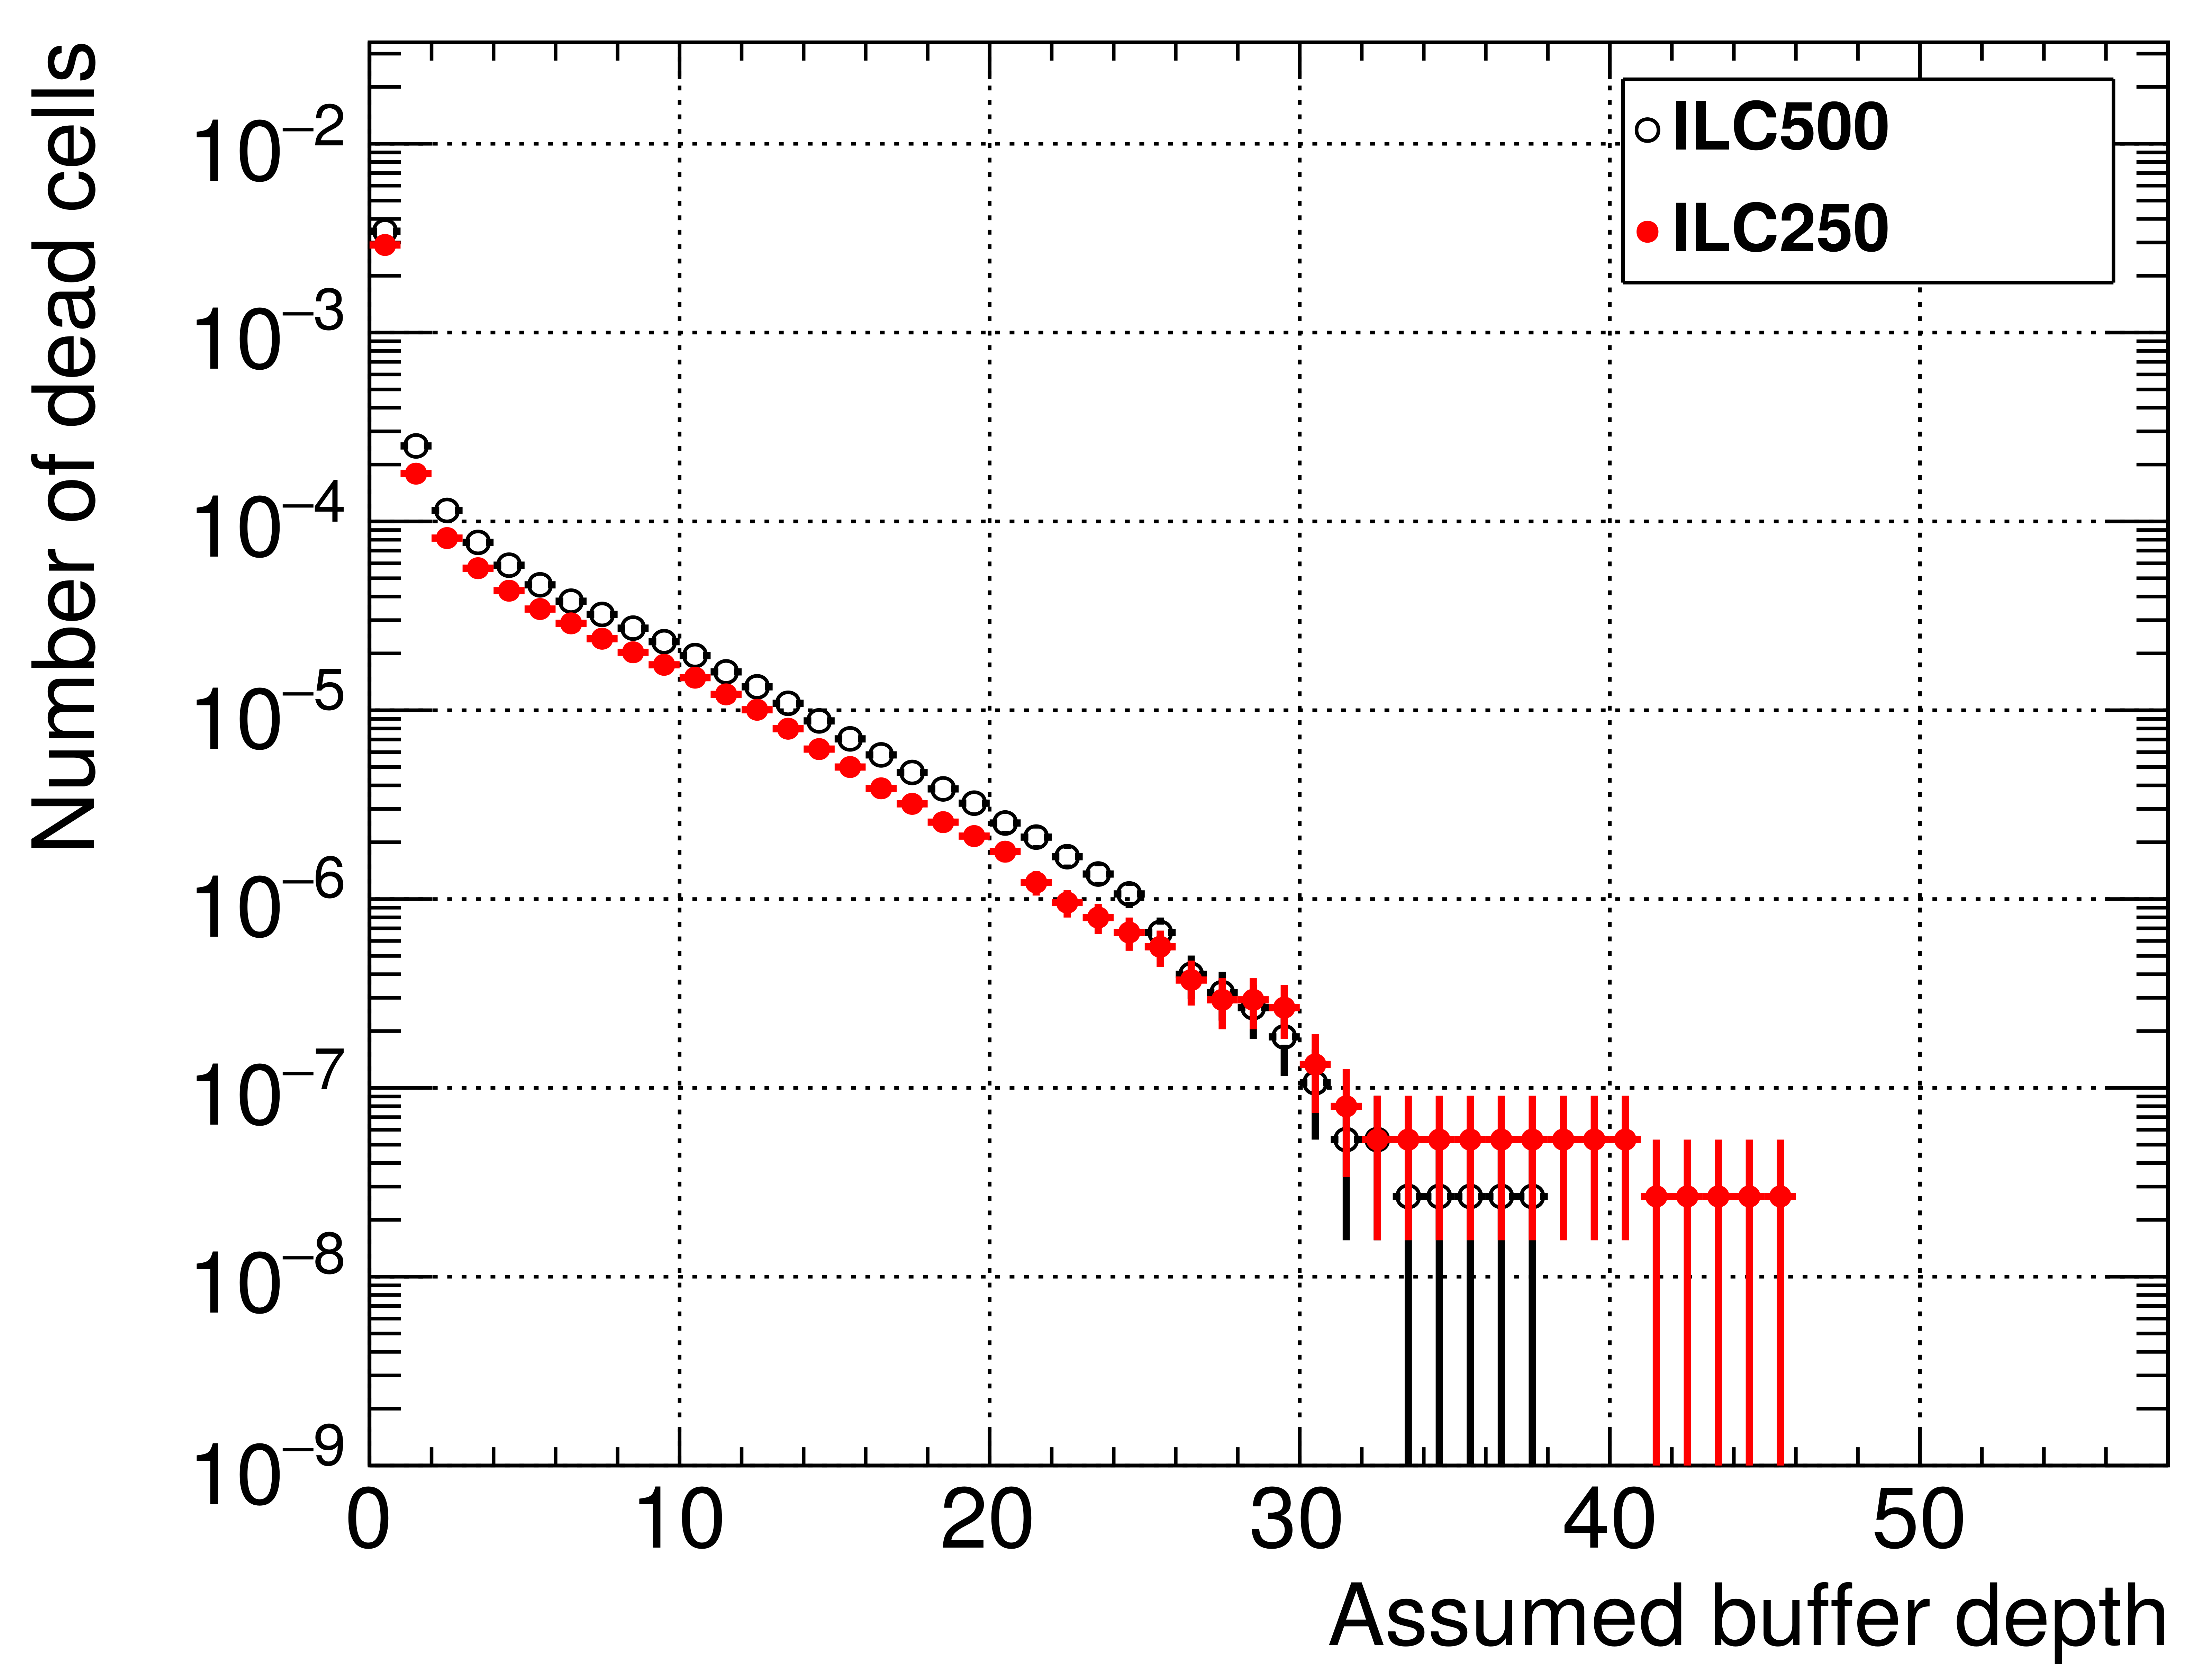
\includegraphics[width=\textwidth]{Figures/Pairs/Occupancy_Comparison_Layer_0_deadcells_ILC500vsILC250_SiVertexEndcap.png}
   \caption{\sid vertex detector \textbf{endcaps}}
   \end{subfigure}
   \caption[Pair background occupancy in the \sid vertex detector for the ILC500 and the ILC250]{Pair background occupancy for the ILC500 in comparison to the ILC250, for the \textbf{innermost \sid vertex detector layer}, after a full bunch train (\num{1312} bunch crossings).
   In both figures, the ratio of dead cells is shown with respect to the total number of cells of the innermost vertex detector layer.
   Figure (a) shows the results for the vertex detector barrel, Figure (b) shows for the vertex detector endcaps.
   }
   \label{fig:PairBkg:ILC500-ILC250_Occupancy}
\end{figure}
Finally, another dependency factor has not been discussed yet, namely the dependency on the number of beam bunches per train.
The ILC stages in all studies presented so far have \num{1312} bunches per train.
The ``Lumi Up'' stage, which is listed in Table~\ref{tab:ILC_parameters}, is an ILC stage with a center-of-mass energy of \SI{500}{\GeV} and an upgraded luminosity.
The luminosity of this stage is doubled with respect to the ILC500 stage by approximately doubling the number of bunches per train to \num{2625}.
Figure~\ref{fig:PairBkg:ILC500-ILC500LumiUp_Occupancy} shows the resulting pair background occupancy in the innermost layer of the vertex detector barrel and endcaps.
The number of dead cells for a given buffer depth is doubled in both subdetectors for the ``Lumi Up'' stage.
The number of beam bunches therefore also has a direct impact on the pair background and the \sid occupancy.
  \begin{figure}
 \centering
  \begin{subfigure}[b]{0.49\textwidth}
   \centering
    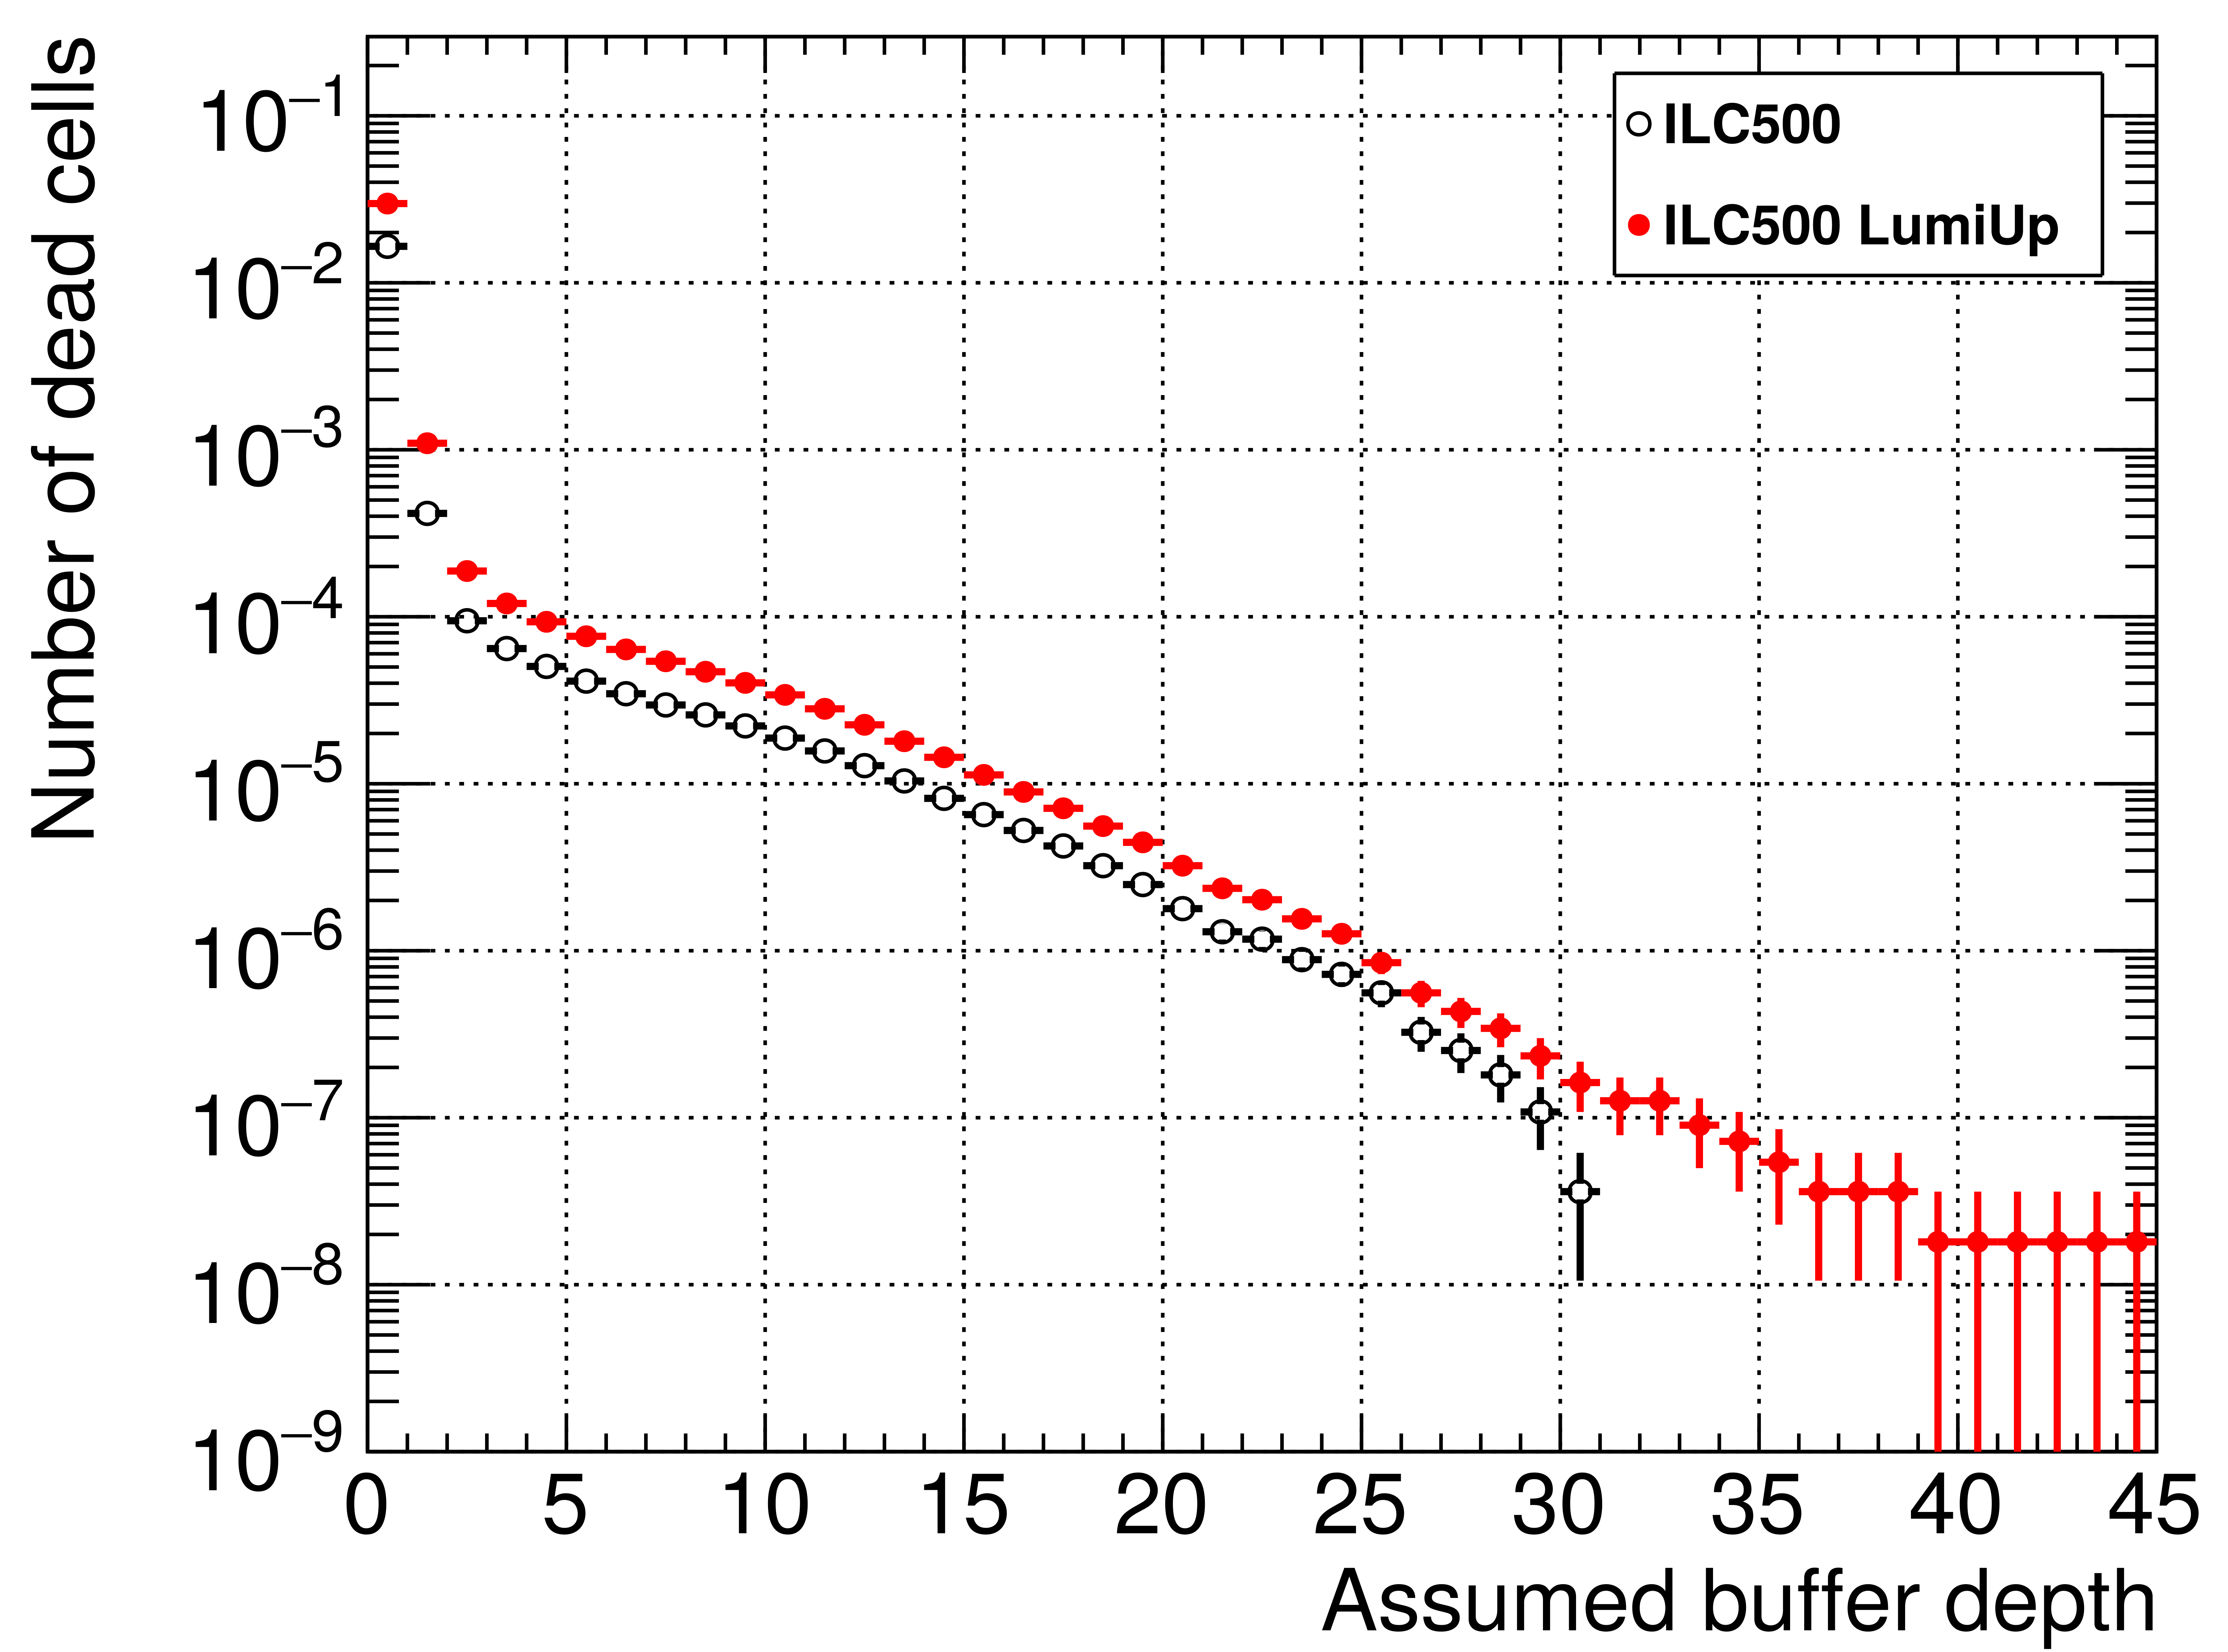
\includegraphics[width=\textwidth]{Figures/Pairs/Occupancy_Comparison_Layer_0_deadcells_ILC500_LumiUp.png}
   \caption{\sid vertex detector \textbf{barrel}}
   \end{subfigure}
   \hfill
    \begin{subfigure}[b]{0.49\textwidth}
   \centering
    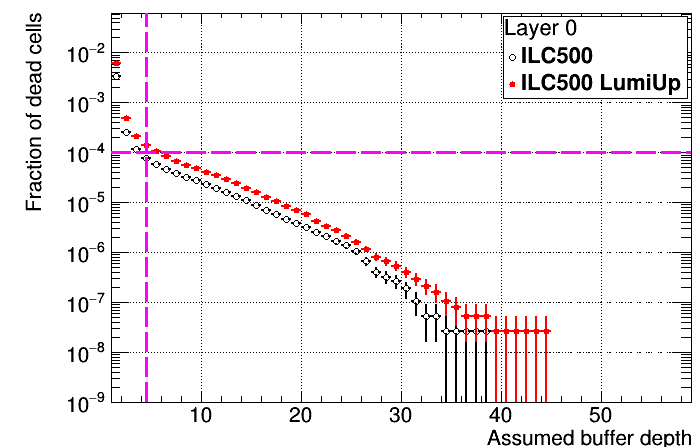
\includegraphics[width=\textwidth]{Figures/Pairs/Occupancy_Comparison_Layer_0_deadcells_ILC500_LumiUp_SiVertexEndcap.png}
   \caption{\sid vertex detector \textbf{endcap}}
   \end{subfigure}
   \caption[Pair background occupancy in the \sid vertex detector for the ILC500 and the ILC500 ``Lumi Up'']{Pair background occupancy for the ILC500 in comparison to the ILC500 luminosity upgrade stage, for the \textbf{innermost \sid vertex detector layer}, after a full bunch train of \num{1312}/\num{2625} bunch crossings.
   In both figures, the ratio of dead cells is shown with respect to the total number of cells of the innermost vertex detector layer.
   Figure (a) shows the results for the vertex detector barrel, Figure (b) for the vertex detector endcaps.
   }
   \label{fig:PairBkg:ILC500-ILC500LumiUp_Occupancy}
 \end{figure}
 
\section{Conclusion}
The pair background arises from the interaction between the electromagnetic fields of the colliding beam bunches.
These interactions are dependent on the ILC beam parameters, which therefore affect the pair background characteristics.
This chapter has also shown that the pairs, which originate from the IP as well as backscatter from the BeamCal, populate the inner \sid subdetectors.
Especially in the vertex detector, it is crucial to investigate the impact of the beam parameters in great detail.
As the width of the pair background envelopes varies and the tracks of the pairs reaches towards the innermost vertex detector layers, the occupancy is directly affected by the change in the beam parameters.
The presented studies have shown that the occupancy from the pair background does not only depend on the beam parameters, but also on the center-of-mass energy, the number of beam bunches per train, and the \sid detector geometry.
These findings are a valuable input to design decisions regarding the ILC accelerator and the \sid detector, and were already consulted for the Change Request decision of the new beam parameters for the ILC stage at a center-of-mass energy of \SI{250}{\GeV}.